\ifdefined\embeddedappendix
\else
\documentclass[10pt]{article}
\usepackage{times}
\usepackage{mathptmx}

\usepackage[margin=0.50in]{geometry}
\usepackage{amsmath}
\usepackage{array}
\usepackage{booktabs}
\usepackage{enumitem}
\usepackage{hyperref}
\usepackage{apacite}
\usepackage{longtable}
\usepackage{microtype}
\usepackage{pdflscape}
\usepackage{graphicx}
\usepackage{tikz}
\usetikzlibrary{arrows.meta,calc,positioning,shapes.geometric}
\hypersetup{hidelinks}

\title{Supplementary Material: Pathway-Centric Evaluation of Synthetic Educational Time-Series Data}
\author{}
\date{}

\emergencystretch=2em
\newcommand{\R}{\mathcal{R}}
\newcommand{\SYN}{\mathcal{S}}
\newcommand{\MAE}{\operatorname{MAE}}
\newcommand{\JS}{\operatorname{JS}}
\newcommand{\NMI}{\operatorname{NMI}}
\newcommand{\msd}[2]{\ensuremath{#1 \mathbin{\pm} #2}}
\newcommand{\msdn}[3]{\ensuremath{#1 \mathbin{\pm} #2_{\scriptscriptstyle n=#3}}}
\newcommand{\bmsd}[2]{\ensuremath{\mathbf{#1 \mathbin{\pm} #2}}}
\renewcommand{\thetable}{S\arabic{table}}
\renewcommand{\thefigure}{S\arabic{figure}}

\begin{document}
\maketitle
\appendix
\fi

\section{How to Read This Supplement}

In this supplement, a trajectory is one learner's event sequence (one course
enrollment in OULAD), while a pathway is a behavioral pattern identified by a
rule that multiple trajectories can share. The main paper organizes evaluation
around five learning-analytics questions:
what occurs in the data, how learning unfolds, who is represented, what
analysts can learn from the synthetic data, and what information might be
exposed.  This supplement provides the complete operational detail behind those
questions.  Sections~\ref{sec:symbols}--\ref{sec:dictionary} define every
publication metric, including its intuition, direction, scope, and conditions
under which it is not estimable.  Section~\ref{sec:complete-results} then lists
every numeric entry in the nine final \texttt{publication\_metrics\_v2}
multi-seed summaries.  Section~\ref{sec:statuses} retains outcome-model
collapse, a compact rare-pathway shape-support summary, and the complete
dataset-by-metric applicability contract.  The accompanying
\texttt{rare-shape-estimability.csv} retains every seed-level support decision
and its real/synthetic learner counts. Thus an absent numeric row is never left
for the reader to interpret as either zero or an undocumented omission.

The final benchmark contains three datasets (ASSISTments, EdNet, and OULAD),
three generators (Markov, sequence VAE, and TimeGAN), and the fixed seeds
20260703, 20260704, and 20260705.  All reported standard deviations are
population standard deviations across those generator seeds. Single-run entries
are labeled ``one available run'' without an SD; the missing-run count remains
explicit. Undefined values are never replaced by zero.

\section{Implementation and Reproducibility Details}
\label{sec:implementation}

\paragraph{Trajectory frames and postprocessing.}
ASSISTments models skill, correctness, attempt, hint, response-time, and
opportunity bins. EdNet models question, correctness, elapsed-time,
timestamp-gap, attempt, and hint bins; deterministic question metadata are
rebuilt from the generated question identifier. OULAD is an explicit weekly
panel. Its generator-fitting frame contains course, dominant activity,
registration, click, active-day, and profile attributes. Generated profile
values, derived fields, and terminal outcomes are handled by the common
train-fitted postprocessor detailed below. Learner identifiers and event order
mark boundaries only and are excluded from the learned value representation.
Table~\ref{tab:supp-data-contract}
states the complete implemented contract rather than only the fields retained
in the final normalized output.

\begingroup
\scriptsize
\setlength{\tabcolsep}{3pt}
\begin{longtable}{@{}p{1.75cm}p{1.75cm}p{2.15cm}p{2.15cm}p{4.55cm}p{4.35cm}@{}}
\caption{Processed-data and generator column contract. Learner counts refer to trajectory identifiers; for OULAD these are course enrollments, while the split itself is by physical student. Structural fields establish sequence boundaries and are not learned values.}\label{tab:supp-data-contract}\\
\toprule
Dataset & Split unit & Train/test trajectories & Train/test rows & Generator-fitted value columns & Rebuilt, replaced, or constructed after generation \\
\midrule
\endfirsthead
\toprule
Dataset & Split unit & Train/test trajectories & Train/test rows & Generator-fitted value columns & Rebuilt, replaced, or constructed after generation \\
\midrule
\endhead
\bottomrule
\endlastfoot
ASSISTments & Learner ID & 3,429 / 788 & 282,118 / 64,742 & 6: skill ID, correctness, attempt bin, hint bin, response-time bin, opportunity bin & Learner ID and zero-based event order are newly assigned structural fields. \\
EdNet & Learner ID & 7,703 / 1,963 & 1,021,565 / 264,798 & 6: question ID, correctness, elapsed-time bin, timestamp-gap bin, attempt bin, hint bin & Skill ID and part are deterministically rebuilt from question ID; learner ID and order are newly assigned. \\
OULAD & Physical student ID & 26,072 / 6,521 & 743,533 / 187,324 & 13: course ID, dominant activity, registration, click bin, active-days bin, and eight profile attributes & Module and presentation from course; engagement and gap from generated behavior; profiles independently resampled; dropout, failure, and final result constructed; learner ID and week order newly assigned. \\
\end{longtable}
\endgroup

\paragraph{OULAD shared postprocessor.}
Normalization uses only the real-training split as reference and runs in a fixed
order. First, course identifier is made learner-static and every retained
enrollment-week is marked registered. The eight generated profile fields are
then discarded. For each synthetic learner and each field independently, one
value is sampled with replacement from real-training learners in the same
course; the full real-training profile pool is the fallback for an unseen
course. This targets, and preserves in expectation, course-conditional
univariate marginals without copying one complete real profile as a unit.
Module and presentation are rebuilt from course;
engagement is one exactly when click intensity is nonzero and the learner is
registered. Non-engaged weeks receive activity \texttt{none} and zero active
days, an engaged week decoded with zero active days is repaired to the
\texttt{1--2} bin, and gap categories are recomputed from weeks since the most
recent engaged week.

Dropout, failure, and final result are never generator inputs. A class-balanced
logistic dropout ranker is fitted on real-training learners using course plus
the mean and standard deviation of engagement after the first four observed
weeks; missing post-prefix summaries are set to zero. The predictor features
exclude terminal labels, total trajectory length, and behavior from the
four-week prediction prefix; real dropout is used only as the fitting target.
The frozen model ranks synthetic learners within course, with seeded random
tie-breaking, and assigns the rounded product of the real-training course
dropout rate and the number of synthetic learners in that course (using the
global training rate if a course rate is unavailable). Dropouts receive
\texttt{Withdrawn} and failure zero. Among
completers, the lowest mean generated engagement values are assigned
\texttt{Fail} to match the real-training course failure rate; among the
remaining learners, the highest engagement values receive \texttt{Distinction}
to match the real-training course distinction rate, and the remainder receive
\texttt{Pass}. These labels are pipeline constructs, so OULAD outcome tasks
evaluate the complete generation-and-postprocessing pipeline rather than direct
outcome generation.

\paragraph{Generator settings.}
The Markov baseline is an order-2 tuple n-gram with minimum context count two
and unigram backoff. The sequence VAE uses categorical windows of length 20,
two 256-unit hidden layers, latent dimension 16, learning rate 0.001, KL weight
1.0, and sampling temperature 1.0. The external SynthCity TimeGAN uses
boundary-safe length-20 categorical windows, one 50-unit generator layer, one
50-unit discriminator layer, RNN mode, and CPU execution. Both neural models
receive all available training trajectories, use a batch-size cap of 200 and at
most 100 observed categories per modeled column plus an \texttt{<other>}
category when needed, and have a 50-epoch ceiling. The
effective epoch count is chosen so fitting does not exceed approximately 4,000
minibatch updates. The effective settings, library version, source
hashes, preprocessing and input hashes, and synthetic-output hash are recorded
in each run report. A contiguous block-bootstrap generator remains in the
software only as a copying-sensitive diagnostic; it is not one of the three
ranked generators and is not proposed for privacy-safe release.

\paragraph{Targeting and output budgets.}
The targeted fit forms the union of eligible real-training pathway learners and
assigns each learner three times the sampling weight of other learners;
membership in multiple pathways does not compound the weight. This factor is
fixed across datasets, generators, pathways, and seeds and is not tuned against
evaluation outcomes. ASSISTments targets high hint use, late correctness
decline, persistent low correctness, rapid low-accuracy responding, rare skill
path, and recovery; EdNet uses the same set except high hint use; OULAD targets late
disengagement, rare activity path, and reengagement. The selected unions contain
545 ASSISTments learners (15.89\%), 1,790 EdNet learners (23.24\%), and 2,968
OULAD enrollments (11.38\%). Standard and targeted outputs have identical
learner and row budgets. All generators use the same train-fitted,
mean-calibrated truncated-lognormal length sampler; no individual real learner
length is copied or empirically resampled. For neural outputs, the implementation allocates enough independently generated 20-observation windows to each learner, concatenates them in order, and truncates the final window to the sampled trajectory length. Cross-window continuity is not modeled by this assembly.

\paragraph{Evaluation sampling and uncertainty.}
Memory-heavy fidelity and privacy diagnostics use a deterministic whole-learner
sample capped at 4,000 learners and 120,000 rows per split; source detection
uses at most 100,000 rows per class. Rare-group prevalence and shape and the
primary downstream tasks use the complete processed frames. Nearest-neighbor
queries use at most 1,000 synthetic trajectories against the complete evaluated
real-train reference; membership inference uses at most 1,000 members,
nonmembers, and synthetic reference trajectories. The pipeline uses 200
learner-clustered percentile-bootstrap resamples for threshold-free downstream
scores and paired differences. For OULAD, clusters are course-enrollment
trajectory identifiers (module, presentation, and student ID), not physical
students. All prediction rows within a sampled enrollment are retained together;
different enrollments of the same student are not resampled jointly. The
additional outcome tasks have one prediction row per enrollment. Rare-group prevalence uses an independent
learner-membership bootstrap; conditional shape resamples qualifying learners,
capped at 300 per side. Quantities below declared learner or class-count minima
are reported as not estimable rather than replaced by zero.

\paragraph{Authoritative reports and schema.}
\begin{sloppypar}
The final paired reports are under
\path{experiments/reports/standard_vs_tail_targeted/<dataset>/<model>/}.
Dataset keys are \path{assistments_2009_2010_skill_builder},
\path{ednet_kt1}, and \path{oulad_weekly_engagement}; model keys are
\path{markov_ngram}, \path{sequence_vae_timevae}, and
\path{timegan}. Each \path{seed_<seed>/generation_evaluation_report.json}
contains the seed-level result, and \path{multi_seed_summary.json} contains
the aggregate. The immutable \texttt{experiments/reports/standard/} directory
is the RQ1 audit snapshot; it is neither averaged into the paired results nor
counted as additional runs. Runtime manifests are under the corresponding
\texttt{experiments/runs/} tree and are git-ignored.

Seed reports declare
\path{publication.schema_version=publication_metrics_v2}, organize promoted
results under \path{publication.metrics.rq1} and
\path{publication.metrics.rq2}, retain exact
exclusions and reasons under
\path{publication.excluded_from_publication}; every
\path{final_audit.status} must equal \path{passed} with an empty issues list.
Aggregates declare
\path{publication_schema_version=publication_metrics_v2} and
\path{metric_summary_scope=publication_only}. Their flattened numeric paths
retain mean, population SD, minimum, maximum, estimable-seed count, and missing
runs; \path{publication_status_summary} retains nonnumeric collapse and support
states with their exact seeds.
The deterministic learner split uses seed 20260703, and generator seeds are
20260703, 20260704, and 20260705. Seed-level bootstrap intervals remain in the
seed reports and are not averaged.
\end{sloppypar}

\section{Notation and Shared Comparison Measures}
\label{sec:symbols}

Let \(\R\) denote the real reference trajectories and \(\SYN\) the synthetic
trajectories.  Learner \(i\)'s ordered trajectory is
\(x_i=((z_{it},c_{it},\mathbf{v}_{it},\theta_{it}))_{t=1}^{T_i}\).  The
primary binary behavior is \(z\): correctness in ASSISTments and EdNet and
weekly engagement in OULAD.  The categorical event type \(c\) is a skill,
question, or activity.  The vector \(\mathbf{v}\) contains the other modeled
signals, and \(\theta\) is event time or week when a meaningful time signal is
available.
Jensen--Shannon divergence follows Lin~\cite{lin1991divergence}; the geometric-mean normalization of mutual information follows Strehl and Ghosh~\cite{strehl2002cluster}; source detectability follows classifier two-sample testing~\cite{lopezpaz2017c2st}; precision--recall and ROC interpretation follows Davis and Goadrich~\cite{davis2006precision}, Saito and Rehmsmeier~\cite{saito2015precision}, and Fawcett~\cite{fawcett2006roc}; train-on-synthetic, test-on-real evaluation follows prior time-series work~\cite{esteban2017realvalued,yoon2019timegan}; and the disclosure audit follows the membership-inference threat model of Shokri et al.~\cite{shokri2017membership} and synthetic-data privacy cautions of Stadler et al.~\cite{stadler2022synthetic}.

\begin{longtable}{@{}p{2.65cm}p{6.15cm}p{6.0cm}@{}}
\caption{Shared notation and comparison functions.}\label{tab:supp-notation}\\
\toprule
Quantity & Definition & Intuition \\
\midrule
\endfirsthead
\toprule
Quantity & Definition & Intuition \\
\midrule
\endhead
\bottomrule
\endlastfoot
Mean absolute error &
\(\MAE(\mathbf a,\mathbf b)=K^{-1}\sum_{k=1}^{K}|a_k-b_k|\). &
Average separation between matched summaries; zero means exact agreement. \\
Jensen--Shannon divergence &
\(\JS(P,Q)=\tfrac12\mathrm{KL}_2(P\Vert M)+\tfrac12\mathrm{KL}_2(Q\Vert M)\), where \(M=(P+Q)/2\). &
Symmetric difference between two discrete distributions.  With base-2 logs it lies in \([0,1]\), and zero means identical distributions. \\
Normalized mutual information &
\(\NMI(X,Y)=I(X;Y)/\sqrt{H(X)H(Y)}\), with zero when either entropy is zero. &
Strength of a categorical relationship after normalizing for the variables' entropies. \\
Normalized trajectory position &
Each learner's primary-behavior sequence is linearly interpolated onto ten positions from beginning to end before learner averaging. &
Compares early-to-late development without allowing longer trajectories to contribute more learners' worth of evidence. \\
Population SD &
\(\sqrt{n^{-1}\sum_{s=1}^{n}(m_s-\bar m)^2}\) over the estimable fixed generator seeds. &
Describes seed-to-seed generator variability; it is not a standard error over learners. \\
\end{longtable}

\section{Complete Metric Dictionary}
\label{sec:dictionary}

The dictionary follows the five questions used in the main paper. Each subsection gives the metric definitions, learning-analytics intuition, preferred direction, and applicability conditions for one evaluation construct.

\subsection{Population Composition: What Occurs?}

The population-composition metrics ask whether synthetic records reproduce the
amount and mixture of observed behavior. Aggregate-behavior checks are
necessary but insufficient because they ignore educational order and learner
pathways.

\begin{longtable}{@{}p{3.5cm}p{6.1cm}p{5.2cm}p{1.4cm}@{}}
\caption{Population-composition metrics.}\label{tab:supp-dictionary-composition}\\
\toprule
Metric & Formal or operational definition & Learning-analytics intuition & Better \\
\midrule
\endfirsthead
\toprule
Metric & Formal or operational definition & Learning-analytics intuition & Better \\
\midrule
\endhead
\bottomrule
\endlastfoot
Behavior-rate error & \(|\bar z_{\R}-\bar z_{\SYN}|\), using event-weighted means.  Because \(z\) is binary, the negative-state error is identical and is not duplicated. & Does the synthetic dataset contain the same overall correctness or engagement rate? & Lower \\
Event-type frequency divergence & \(\JS(P_{\R}(c),P_{\SYN}(c))\). & Does it contain the same mixture of skills, questions, or weekly activity types? & Lower \\
Average feature-distribution divergence & \(J^{-1}\sum_{j=1}^{J}\JS(P_{\R}(v_j),P_{\SYN}(v_j))\) over prespecified generator-modeled attributes. & Are modeled attributes such as attempts, hints, timing bins, or activity intensities present in realistic proportions? & Lower \\
Real-versus-synthetic detectability AUROC & \(\max(A,1-A)\), where \(A\) is AUROC of a classifier distinguishing real from synthetic event records. Detector partitions are learner-disjoint. & Can a classifier easily tell which modeled records are artificial without seeing records from the same learner on both sides? A value of 0.5 is chance-level indistinguishability; 1 is perfect separation. & 0.5 \\
\end{longtable}

\subsection{Learning Process: How Does Learning Unfold?}

This group tests temporal order, progression, persistence, spacing, and
relationships among educational signals.  It distinguishes a realistic bag
of events from a realistic learning trajectory.

\begin{longtable}{@{}p{3.5cm}p{6.1cm}p{5.2cm}p{1.4cm}@{}}
\caption{Learning-process metrics.}\label{tab:supp-dictionary-process}\\
\toprule
Metric & Formal or operational definition & Learning-analytics intuition & Better \\
\midrule
\endfirsthead
\toprule
Metric & Formal or operational definition & Learning-analytics intuition & Better \\
\midrule
\endhead
\bottomrule
\endlastfoot
Behavior-transition divergence & \(\JS\) between pooled within-learner adjacent pairs \((z_t,z_{t+1})\). & Are persistence, recovery, and decline transitions produced at realistic rates? & Lower \\
Three-event sequence divergence & \(\JS\) between pooled within-learner event-type triples \((c_t,c_{t+1},c_{t+2})\).  Windows never cross learner boundaries. & Are short ordered skill or activity motifs realistic? & Lower \\
Trajectory-shape error & \(10^{-1}\sum_{b=1}^{10}|q_{\R}(b)-q_{\SYN}(b)|\), where \(q_D(b)\) is the learner-averaged primary behavior at normalized position \(b\). & Does the average trajectory rise, fall, or recover in the right way from beginning to end? & Lower \\
Behavior-persistence error & \(3^{-1}\sum_{\ell\in\{1,2,3\}}|\rho_{\R}(z_t,z_{t+\ell})-\rho_{\SYN}(z_t,z_{t+\ell})|\). & Do correct/incorrect or engaged/disengaged states form similarly persistent streaks? & Lower \\
Response/inactivity-gap distribution divergence & \(\JS(P_{\R}(g),P_{\SYN}(g))\). In EdNet, \(g\) is binned elapsed time since the prior response; in OULAD, it is binned weeks since the most recent engaged week. It is not applicable in ASSISTments. & Does the generator preserve response spacing or inactivity history, rather than response duration within one event? & Lower \\
Behavior--hint lag error & Mean absolute difference in \(\rho(z_t,h_{t+\ell})\) for \(\ell\in\{0,1\}\).  It is not estimated if hint use is absent or constant. & Is help-seeking related to current and next-step performance in the same way? & Lower \\
Feature-dependence error & Mean absolute real--synthetic NMI difference over prespecified scientifically relevant signal pairs. & Are relationships among modeled signals retained even if individual columns look realistic? & Lower \\
\end{longtable}

\subsection{Learner-Pathway Representation: Who Is Represented?}

This group asks whether common learner strata and uncommon but
intervention-relevant pathways appear in realistic proportions, and whether
learners in those groups show realistic later behavior. Prefix-defined subgroups use a rule fitted on real
training data and evaluate only later observations.  Rare-group rules and
thresholds are also fitted only on real training data and then applied
unchanged to synthetic and held-out real learners.

\begin{longtable}{@{}p{3.5cm}p{6.1cm}p{5.2cm}p{1.4cm}@{}}
\caption{Learner-pathway representation metrics.}\label{tab:supp-dictionary-pathways}\\
\toprule
Metric & Formal or operational definition & Learning-analytics intuition & Better \\
\midrule
\endfirsthead
\toprule
Metric & Formal or operational definition & Learning-analytics intuition & Better \\
\midrule
\endhead
\bottomrule
\endlastfoot
Subgroup behavior error & MAE across fixed prefix-defined groups in their later primary-behavior rates. & Do learners with different early histories show realistic later correctness or engagement? & Lower \\
Subgroup-size error & MAE across the same groups in learner share. & Does the generator produce the same mixture of early-history learner types? & Lower \\
Subgroup hint-use error & MAE across eligible groups in later hint-request rates; not estimated without a varying hint signal. & Do early-history learner groups retain their later help-seeking behavior? & Lower \\
Rare-group prevalence error & For group \(g\), \(|\pi_g(\R)-\pi_g(\SYN)|\), where \(\pi_g(D)\) is learner prevalence. & Does the generator include the right fraction of learners following a rare pathway? & Lower \\
Signed rare-group prevalence difference & For group \(g\), \(\pi_g(\SYN)-\pi_g(\R)\).  It is reported in percentage points alongside the absolute error. & Is the pathway underrepresented (negative), accurately represented (near zero), or overrepresented (positive)? & Zero \\
Rare-group trajectory-shape error & Trajectory-shape error recomputed among learners satisfying \(g\).  It requires at least ten qualifying real and ten qualifying synthetic learners. & Conditional on producing the group, does correctness or engagement among qualifying learners develop realistically? & Lower \\
\end{longtable}

Distribution-based rarity rules target the outer 5\% of the real-training distribution. The
10\% ceiling allows for ties in discretized variables without treating a common
behavior as rare. Fixed change thresholds and minimum lengths are benchmark
defaults for interpretable behavioral contrasts, not universal educational cut
points. Prevalence remains reportable when no or too few synthetic learners qualify,
because absence is itself a representation result.  Shape is marked not estimable
when either arm has fewer than ten qualifying learners.  Publication rare
groups have complete-real-training learner prevalence at most 10\%.  The
published groups are high hint use, late correctness decline, persistent low
correctness, rapid low-accuracy responding, rare skill path, and recovery where applicable; OULAD uses late
disengagement, rare activity path, and reengagement.  A coarse binned signal is
excluded if no strict or inclusive boundary yields a nonempty group within the
rarity ceiling.

Rare skill/activity paths are scored by the mean log$_2$ probability of successive skill/activity transitions under a real-training transition model with add-one smoothing. The bottom 5\% defines the candidate rare-pathway group, subject to the rarity ceiling and at least one observed transition.

\subsection{Analytic Usefulness: What Can Analysts Learn?}

The main paper's prediction-specification table lists the actual predictor inputs, fixed early-history lengths, and numerical eligibility requirements. Every downstream predictor is evaluated on the same held-out real learners.
The primary task is next-response correctness for ASSISTments and EdNet and
next-week engagement for OULAD.  The five training arms are real only (TRTR),
standard synthetic only (TSTR), real plus standard synthetic, pathway-targeted
synthetic only, and real plus pathway-targeted synthetic.  Learner-level outcome
tasks use four arms because real plus targeted synthetic is not defined there.
In synthetic-only arms, no real outcome rows fit the predictor, although all
arms use the same real-training-fitted schema and transformations. AUPRC and
AUROC are computed over eligible prediction rows, so longer trajectories
contribute more instances; learner-clustered bootstrapping preserves within-
learner dependence without changing that event-weighted point estimate.

\begin{longtable}{@{}p{3.5cm}p{6.1cm}p{5.2cm}p{1.4cm}@{}}
\caption{Analytic-usefulness metrics and contrasts.}\label{tab:supp-dictionary-utility}\\
\toprule
Metric & Formal or operational definition & Learning-analytics intuition & Better \\
\midrule
\endfirsthead
\toprule
Metric & Formal or operational definition & Learning-analytics intuition & Better \\
\midrule
\endhead
\bottomrule
\endlastfoot
AUPRC & Area under the precision--recall curve on held-out real data.  The observed positive rate is the no-skill reference. & Primary score for imbalanced educational outcomes and rare learner slices; rewards identifying positives without many false alarms. & Higher \\
AUROC & Probability that a randomly chosen positive receives a higher score than a randomly chosen negative. & Secondary threshold-free discrimination score; less sensitive than AUPRC to positive-class prevalence. & Higher \\
Standard synthetic utility loss & \(M_{\rm TRTR}-M_{\rm standard}\), separately for AUPRC and AUROC. & How much held-out-real predictive performance is lost when analysts train only on ordinary synthetic data? & Lower \\
Standard augmentation gain & \(M_{\rm real+standard}-M_{\rm TRTR}\). & Does adding ordinary synthetic data improve a predictor already trained on real data? & Higher \\
Targeted-vs-standard TSTR gain & \(M_{\rm targeted}-M_{\rm standard}\). & Does emphasizing rare training learners make synthetic-only data more useful? & Higher \\
Targeted augmentation gain & \(M_{\rm real+targeted}-M_{\rm TRTR}\). & Does pathway-targeted synthetic augmentation improve over real-only training? & Higher \\
Pathway-level predictive usefulness & The same five arms and four contrasts, evaluated only on held-out real learners satisfying a fixed rare-group rule. & Can a model trained on synthetic data learn the signal needed for uncommon, educationally consequential learner pathways? & Varies \\
Rare-group prevalence-match change & \(E^{\rm prev}_{\rm standard}-E^{\rm prev}_{\rm targeted}\). & Did targeting move the learner proportion closer to its real-training reference, without treating overproduction as success? & Higher \\
Rare-group shape-error reduction & \(E^{\rm shape}_{\rm standard}-E^{\rm shape}_{\rm targeted}\), only when both errors are estimable. & Did targeting improve the group's within-trajectory primary-behavior pattern? & Higher \\
Learner-level outcome-task AUPRC/AUROC and contrasts & Persistent-low-correctness and recovery prediction in ASSISTments/EdNet; dropout and course-failure prediction in OULAD, using only declared early history. & Does synthetic data support intervention-oriented outcomes beyond the primary next-step prediction task? & Varies \\
\end{longtable}

OULAD terminal labels are excluded from generator inputs and constructed by the
common leakage-safe post-generation pipeline. These pipeline-level outcome tasks
evaluate the complete synthetic-data pipeline, not direct generation of future
outcomes. The machine-readable reports retain the corresponding internal scope
code for auditability.

\subsection{Disclosure Risk: What Might Be Exposed?}

These measures are empirical memorization audits, not differential-privacy
guarantees.  A large nearest-neighbor distance should not be maximized without
regard to fidelity: unrelated noise can be far from training data while being
useless.

\paragraph{Trajectory representation and distance.}
Each event is represented by the tuple of all nonidentifier, non-order audit
columns shared by the normalized real and synthetic frames. For trajectories
$x=(u_1,\ldots,u_{T_x})$ and $y=(v_1,\ldots,v_{T_y})$, the implemented
positional distance is
\[
d(x,y)=\frac{|T_x-T_y|+
\sum_{t=1}^{\min(T_x,T_y)}\mathbf{1}[u_t\ne v_t]}
{\max(T_x,T_y)}.
\]
Distance is zero when both trajectories are empty. An aligned position counts
as one mismatch when its complete event tuple differs, regardless of how many
fields differ, and unmatched suffix positions count through the length term.
Thus $d\in[0,1]$, with no temporal realignment and $d=0$ indicating an exact
normalized audit-trajectory match.

\paragraph{Near-copy and membership rules.}
The threshold \(\tau=0.1\) is fixed for every dataset, generator, arm, and seed.
Under this distance, $d\leq0.1$ means that at least 90\% of positions in the
longer trajectory match exactly after counting length mismatch. This is a
prespecified benchmark flag, not a literature-derived or validated privacy
boundary. The membership attack gives each real learner the fixed score
$-\min_{z\in\SYN}d(x,z)$, so greater proximity always means ``more likely a
training member.'' A below-chance AUROC is not inverted after seeing the labels;
reported advantage is \(\max\{0,2(A-0.5)\}\). For copying and membership,
targeting risk change is targeted minus standard; for mean distance it is
standard minus targeted, so positive values consistently indicate greater
empirical exposure after targeting. Sampling limits and bootstrap counts are
given in Section~\ref{sec:implementation}.

\begin{longtable}{@{}p{3.5cm}p{6.1cm}p{5.2cm}p{1.4cm}@{}}
\caption{Disclosure-risk metrics.}\label{tab:supp-dictionary-privacy}\\
\toprule
Metric & Formal or operational definition & Learning-analytics intuition & Safer \\
\midrule
\endfirsthead
\toprule
Metric & Formal or operational definition & Learning-analytics intuition & Safer \\
\midrule
\endhead
\bottomrule
\endlastfoot
Exact-duplicate rate & Fraction of synthetic learners whose full normalized audit trajectory exactly matches a real-training trajectory. & How often does the generator literally reproduce a learner's normalized sequence over the audit columns? & Lower \\
Near-duplicate rate & Fraction of synthetic trajectories with \(\min_{r\in\R}d(x,r)\leq\tau\), where \(\tau=0.1\). & How often does the generator produce a trajectory unusually close to one seen in training? & Lower \\
Mean nearest-training distance & Mean \(\min_{r\in\R}d(x,r)\) over evaluated synthetic trajectories. & On average, how closely does each synthetic learner resemble its nearest training learner? & Higher \\
Membership-inference advantage & \(\max(0,2(A-0.5))\) for the fixed proximity-oriented attack AUROC \(A\). & Can an attacker distinguish training learners from held-out learners using proximity to the synthetic data? & Lower \\
Behavior-projection exact-duplicate rate & Exact-copy rate after projecting OULAD to ordered dominant-activity/engagement pairs. & How often are weekly behavioral patterns repeated when independently assigned profiles and constructed outcomes are removed? & Lower \\
Targeted-minus-standard privacy-risk change & Targeted minus standard for copy and membership metrics; for distance, standard distance minus targeted distance so positive always means greater exposure. & Did pathway targeting make the empirical memorization signal stronger? & Lower \\
\end{longtable}

OULAD full-record nearest-neighbor and membership comparisons are excluded
because demographic profiles are independently sampled and terminal outcomes
are constructed after generation. Only exact copying on the ordered
dominant-activity/engagement projection is promoted for comparison. Exploratory
pathway-specific privacy blocks remain in raw reports, but the publication audit
is deliberately dataset-level and does not estimate risk specifically for
uncommon pathways.

\section{Applicability, Uncertainty, and Exclusions}

Metrics use the real training split as the fidelity reference because
generators are trained on the real-training distribution. Preprocessing transforms, category
maps, trajectory-length models, rare-group thresholds, subgroup cut points,
postprocessors, and targeting membership are fit without held-out real test
learners.  Downstream evaluation uses held-out real learners only.  OULAD is
split by physical student, preventing different course enrollments from the
same student from crossing the train/test boundary.

All numeric tables report means and population SD over fixed generator seeds.
Seed-level bootstrap intervals over held-out learners remain in the JSON seed
reports and are not averaged across seeds. Bootstrap intervals quantify
learner-sampling uncertainty conditional on one fixed generated dataset and
seed, whereas cross-seed SD describes generator stochasticity. With three
generator seeds and one fixed learner-disjoint split, the paper treats
cross-seed differences descriptively; neither summary captures split-to-split
variability. A metric based on a constant or absent signal is not applicable. A
rare-group conditional metric is not estimable below its declared support.
Model-collapse outcomes are preserved as statuses. Table~\ref{tab:supp-exclusions}
lists every exclusion category present in the final seed reports. The
seed-level source of truth is
\texttt{publication.excluded\_from\_publication}; exclusion from comparison is
distinct from non-estimability, whose support or class status remains a
publication result.

\begingroup
\scriptsize
\setlength{\tabcolsep}{3pt}
\begin{longtable}{@{}p{4.15cm}p{5.15cm}p{6.2cm}@{}}
\caption{Complete publication-exclusion dictionary. Dataset-specific omitted-group reasons and fitted prevalences remain verbatim in each seed report.}\label{tab:supp-exclusions}\\
\toprule
Report exclusion key & Excluded item & Reason \\
\midrule
\endfirsthead
\toprule
Report exclusion key & Excluded item & Reason \\
\midrule
\endhead
\bottomrule
\endlastfoot
\path{fixed_threshold_classification_scores} & Accuracy, precision, recall, and F1 at an untuned 0.5 threshold & Threshold-free AUPRC and AUROC are the prespecified predictive comparisons. \\
\path{threshold_metric_deltas} & Targeting and augmentation contrasts for fixed-threshold scores & Only AUPRC/AUROC gaps are promoted. \\
\path{lightweight_downstream_utility} & Skill-mean probability baseline & It is a smoke-test diagnostic superseded by the declared histogram-gradient-boosting model. \\
\path{sequence_length_model_ranking} & Length-distribution metrics & All generators use the same train-fitted length sampler, so the result is not architecture-attributable. \\
\path{short_and_long_trajectory_tails} & Length-based uncommon pathways & The shared length sampler prevents generator attribution. \\
\path{diversity_uniqueness_rates} & Raw diversity/coverage, uniqueness, entropy, and cardinality diagnostics & Novelty is not monotonic quality and remains a raw diagnostic. \\
\path{raw_membership_auc_inversion} & Flipping a below-chance membership AUROC & Attack orientation is fixed before labels are inspected; the published advantage is not post-hoc inverted. \\
\path{raw_test_fidelity_duplicates} & Fidelity recomputed against held-out real test & Real train is the generator's fidelity reference; held-out real learners are reserved for generalization and nonmembership evaluation. \\
\path{raw_diagnostic_aggregates} & Unfiltered all-column marginals/dependence, detector accuracy, and minimum-distance extremes & These broad exploratory outputs do not belong to the prespecified construct metrics. \\
\path{omitted_standard_tail_groups} & Inapplicable or unsupported standard-arm pathway blocks & Reasons include absent signals, postprocessed outcomes, and fewer than ten qualifying learners; prevalence is retained when defined. \\
\path{omitted_targeted_tail_groups} & The corresponding targeted-arm pathway blocks & The same frozen applicability and support rules apply to both generation arms. \\
\path{omitted_tail_learnability_groups} & Ineligible held-out-real pathway slices & Groups above the rarity ceiling, outside the dataset semantics, or below predictive support are not included in pathway-level prediction comparisons. \\
\path{unavailable_percentile_tail_groups} & Percentile pathways for which ties cannot yield a nonempty group at or below 10\% & A common discretized behavior is not relabeled as rare. \\
\path{distinguishability} & OULAD full-record source detection & Independently resampled profiles and constructed outcomes confound generator attribution. \\
\end{longtable}
\endgroup

Dataset-specific scope rules add the following consequences. OULAD demographic
subgroup fidelity, postprocessed dropout prevalence/shape, full-record source
detection, and full-record nearest-neighbor/membership privacy are not used for
generator comparison. The diagnostic persistent-misconception rule is omitted
where the dataset does not support that pedagogical interpretation. Only the
prespecified signal pairs, generator-attributable fields, and real-train
fidelity reference enter publication comparisons.

The full applicability grid in Table~\ref{tab:supp-applicability} distinguishes
three cases that would otherwise all appear as missing cells: a metric can be
inapplicable because a required signal is absent or constant, deliberately
excluded because postprocessing prevents a generator-comparable interpretation,
or applicable but not estimable in a particular seed because learner or class
support is insufficient.

\section{Complete Numerical Publication Results}
\label{sec:complete-results}

The following tables contain all 1,451 numeric entries in the nine final
multi-seed publication summaries.  The generation audit verifies equality
between source and emitted row counts. Printed tables show mean, population SD,
estimable-seed count, and missing-seed count. The accompanying
\texttt{supplement-generated/complete-publication-results.csv} also retains the
source minimum, maximum, exact JSON path, and all six summary fields for every
row.

\scriptsize
\setlength{\tabcolsep}{3pt}
\begin{longtable}{@{}p{2.25cm}p{2.05cm}p{4.7cm}p{5.0cm}p{2.6cm}p{1.25cm}@{}}
\caption{Complete publication results for population composition. Every numeric metric-summary entry is shown; SD is the population SD across the fixed seeds and $n$ is the number of estimable seeds.}\label{tab:supp-population-composition}\\
\toprule
Dataset & Generator & Scope / comparison & Metric & Mean $\pm$ SD ($n$) & Direction \\
\midrule
\endfirsthead
\multicolumn{6}{l}{\textit{Continued from previous page}}\\
\toprule
Dataset & Generator & Scope / comparison & Metric & Mean $\pm$ SD ($n$) & Direction \\
\midrule
\endhead
\midrule
\multicolumn{6}{r}{\textit{Continued on next page}}\\
\endfoot
\bottomrule
\endlastfoot
ASSISTments & Markov & All eligible learners/events & Average feature-distribution divergence & $0.0014 \mathbin{\pm} 0.0001$ (3) & Lower \\
ASSISTments & Markov & All eligible learners/events & Behavior-rate error & $0.0120 \mathbin{\pm} 0.0029$ (3) & Lower \\
ASSISTments & Markov & All eligible learners/events & Event-type frequency divergence & $0.0053 \mathbin{\pm} 0.0001$ (3) & Lower \\
ASSISTments & Markov & All eligible learners/events & Real-versus-synthetic detectability AUROC & $0.5334 \mathbin{\pm} 0.0037$ (3) & 0.5 best \\
ASSISTments & SeqVAE & All eligible learners/events & Average feature-distribution divergence & $0.0003 \mathbin{\pm} 0.0000$ (3) & Lower \\
ASSISTments & SeqVAE & All eligible learners/events & Behavior-rate error & $0.0012 \mathbin{\pm} 0.0008$ (3) & Lower \\
ASSISTments & SeqVAE & All eligible learners/events & Event-type frequency divergence & $0.0013 \mathbin{\pm} 0.0001$ (3) & Lower \\
ASSISTments & SeqVAE & All eligible learners/events & Real-versus-synthetic detectability AUROC & $0.8500 \mathbin{\pm} 0.0008$ (3) & 0.5 best \\
ASSISTments & TimeGAN & All eligible learners/events & Average feature-distribution divergence & $0.1907 \mathbin{\pm} 0.0923$ (3) & Lower \\
ASSISTments & TimeGAN & All eligible learners/events & Behavior-rate error & $0.3036 \mathbin{\pm} 0.0745$ (3) & Lower \\
ASSISTments & TimeGAN & All eligible learners/events & Event-type frequency divergence & $0.4101 \mathbin{\pm} 0.1875$ (3) & Lower \\
ASSISTments & TimeGAN & All eligible learners/events & Real-versus-synthetic detectability AUROC & $0.9672 \mathbin{\pm} 0.0214$ (3) & 0.5 best \\
EdNet & Markov & All eligible learners/events & Average feature-distribution divergence & $0.0152 \mathbin{\pm} 0.0000$ (3) & Lower \\
EdNet & Markov & All eligible learners/events & Behavior-rate error & $0.0163 \mathbin{\pm} 0.0013$ (3) & Lower \\
EdNet & Markov & All eligible learners/events & Event-type frequency divergence & $0.0131 \mathbin{\pm} 0.0008$ (3) & Lower \\
EdNet & Markov & All eligible learners/events & Real-versus-synthetic detectability AUROC & $0.5794 \mathbin{\pm} 0.0009$ (3) & 0.5 best \\
EdNet & SeqVAE & All eligible learners/events & Average feature-distribution divergence & $0.0070 \mathbin{\pm} 0.0002$ (3) & Lower \\
EdNet & SeqVAE & All eligible learners/events & Behavior-rate error & $0.0192 \mathbin{\pm} 0.0128$ (3) & Lower \\
EdNet & SeqVAE & All eligible learners/events & Event-type frequency divergence & $0.0020 \mathbin{\pm} 0.0001$ (3) & Lower \\
EdNet & SeqVAE & All eligible learners/events & Real-versus-synthetic detectability AUROC & $0.6894 \mathbin{\pm} 0.0015$ (3) & 0.5 best \\
EdNet & TimeGAN & All eligible learners/events & Average feature-distribution divergence & $0.1197 \mathbin{\pm} 0.0013$ (3) & Lower \\
EdNet & TimeGAN & All eligible learners/events & Behavior-rate error & $0.3345 \mathbin{\pm} 0.0004$ (3) & Lower \\
EdNet & TimeGAN & All eligible learners/events & Event-type frequency divergence & $0.0101 \mathbin{\pm} 0.0001$ (3) & Lower \\
EdNet & TimeGAN & All eligible learners/events & Real-versus-synthetic detectability AUROC & $0.9092 \mathbin{\pm} 0.0008$ (3) & 0.5 best \\
OULAD & Markov & All eligible learners/events & Average feature-distribution divergence & $0.0174 \mathbin{\pm} 0.0003$ (3) & Lower \\
OULAD & Markov & All eligible learners/events & Behavior-rate error & $0.1644 \mathbin{\pm} 0.0038$ (3) & Lower \\
OULAD & Markov & All eligible learners/events & Event-type frequency divergence & $0.0203 \mathbin{\pm} 0.0009$ (3) & Lower \\
OULAD & SeqVAE & All eligible learners/events & Average feature-distribution divergence & $0.0255 \mathbin{\pm} 0.0031$ (3) & Lower \\
OULAD & SeqVAE & All eligible learners/events & Behavior-rate error & $0.0100 \mathbin{\pm} 0.0051$ (3) & Lower \\
OULAD & SeqVAE & All eligible learners/events & Event-type frequency divergence & $0.0231 \mathbin{\pm} 0.0032$ (3) & Lower \\
OULAD & TimeGAN & All eligible learners/events & Average feature-distribution divergence & $0.1605 \mathbin{\pm} 0.1231$ (3) & Lower \\
OULAD & TimeGAN & All eligible learners/events & Behavior-rate error & $0.3494 \mathbin{\pm} 0.1877$ (3) & Lower \\
OULAD & TimeGAN & All eligible learners/events & Event-type frequency divergence & $0.2222 \mathbin{\pm} 0.1331$ (3) & Lower \\
\end{longtable}

\scriptsize
\setlength{\tabcolsep}{3pt}
\begin{longtable}{@{}p{2.25cm}p{2.05cm}p{4.7cm}p{5.0cm}p{2.6cm}p{1.25cm}@{}}
\caption{Complete publication results for learning process. Every numeric metric-summary entry is shown; SD is the population SD across the fixed seeds and $n$ is the number of estimable seeds.}\label{tab:supp-learning-process}\\
\toprule
Dataset & Generator & Scope / comparison & Metric & Mean $\pm$ SD ($n$) & Direction \\
\midrule
\endfirsthead
\multicolumn{6}{l}{\textit{Continued from previous page}}\\
\toprule
Dataset & Generator & Scope / comparison & Metric & Mean $\pm$ SD ($n$) & Direction \\
\midrule
\endhead
\midrule
\multicolumn{6}{r}{\textit{Continued on next page}}\\
\endfoot
\bottomrule
\endlastfoot
ASSISTments & Markov & All eligible learners/events & Feature-dependence error & $0.0017 \mathbin{\pm} 0.0004$ (3) & Lower \\
ASSISTments & Markov & All eligible learners/events & Behavior--hint lag error & $0.0071 \mathbin{\pm} 0.0021$ (3) & Lower \\
ASSISTments & Markov & All eligible learners/events & Behavior-persistence error & $0.0293 \mathbin{\pm} 0.0042$ (3) & Lower \\
ASSISTments & Markov & All eligible learners/events & Trajectory-shape error & $0.0409 \mathbin{\pm} 0.0041$ (3) & Lower \\
ASSISTments & Markov & All eligible learners/events & Behavior-transition divergence & $0.0002 \mathbin{\pm} 0.0001$ (3) & Lower \\
ASSISTments & Markov & All eligible learners/events & Three-event sequence divergence & $0.0828 \mathbin{\pm} 0.0006$ (3) & Lower \\
ASSISTments & SeqVAE & All eligible learners/events & Feature-dependence error & $0.0993 \mathbin{\pm} 0.0000$ (3) & Lower \\
ASSISTments & SeqVAE & All eligible learners/events & Behavior--hint lag error & $0.4437 \mathbin{\pm} 0.0026$ (3) & Lower \\
ASSISTments & SeqVAE & All eligible learners/events & Behavior-persistence error & $0.2017 \mathbin{\pm} 0.0009$ (3) & Lower \\
ASSISTments & SeqVAE & All eligible learners/events & Trajectory-shape error & $0.0272 \mathbin{\pm} 0.0029$ (3) & Lower \\
ASSISTments & SeqVAE & All eligible learners/events & Behavior-transition divergence & $0.0100 \mathbin{\pm} 0.0002$ (3) & Lower \\
ASSISTments & SeqVAE & All eligible learners/events & Three-event sequence divergence & $0.8635 \mathbin{\pm} 0.0032$ (3) & Lower \\
ASSISTments & TimeGAN & All eligible learners/events & Feature-dependence error & $0.1029 \mathbin{\pm} 0.0123$ (3) & Lower \\
ASSISTments & TimeGAN & All eligible learners/events & Behavior--hint lag error & $0.3507 \mathbin{\pm} 0.1340$ (3) & Lower \\
ASSISTments & TimeGAN & All eligible learners/events & Behavior-persistence error & $0.1881 \mathbin{\pm} 0.0192$ (3) & Lower \\
ASSISTments & TimeGAN & All eligible learners/events & Trajectory-shape error & $0.3307 \mathbin{\pm} 0.0760$ (3) & Lower \\
ASSISTments & TimeGAN & All eligible learners/events & Behavior-transition divergence & $0.2366 \mathbin{\pm} 0.1211$ (3) & Lower \\
ASSISTments & TimeGAN & All eligible learners/events & Three-event sequence divergence & $0.7653 \mathbin{\pm} 0.0025$ (3) & Lower \\
EdNet & Markov & All eligible learners/events & Feature-dependence error & $0.0029 \mathbin{\pm} 0.0001$ (3) & Lower \\
EdNet & Markov & All eligible learners/events & Behavior-persistence error & $0.0230 \mathbin{\pm} 0.0014$ (3) & Lower \\
EdNet & Markov & All eligible learners/events & Trajectory-shape error & $0.1550 \mathbin{\pm} 0.0049$ (3) & Lower \\
EdNet & Markov & All eligible learners/events & Behavior-transition divergence & $0.0005 \mathbin{\pm} 0.0001$ (3) & Lower \\
EdNet & Markov & All eligible learners/events & Response/inactivity-gap distribution divergence & $0.0036 \mathbin{\pm} 0.0001$ (3) & Lower \\
EdNet & Markov & All eligible learners/events & Three-event sequence divergence & $0.4438 \mathbin{\pm} 0.0012$ (3) & Lower \\
EdNet & SeqVAE & All eligible learners/events & Feature-dependence error & $0.0088 \mathbin{\pm} 0.0000$ (3) & Lower \\
EdNet & SeqVAE & All eligible learners/events & Behavior-persistence error & $0.0941 \mathbin{\pm} 0.0006$ (3) & Lower \\
EdNet & SeqVAE & All eligible learners/events & Trajectory-shape error & $0.1460 \mathbin{\pm} 0.0126$ (3) & Lower \\
EdNet & SeqVAE & All eligible learners/events & Behavior-transition divergence & $0.0028 \mathbin{\pm} 0.0008$ (3) & Lower \\
EdNet & SeqVAE & All eligible learners/events & Response/inactivity-gap distribution divergence & $0.0008 \mathbin{\pm} 0.0002$ (3) & Lower \\
EdNet & SeqVAE & All eligible learners/events & Three-event sequence divergence & $0.8978 \mathbin{\pm} 0.0003$ (3) & Lower \\
EdNet & TimeGAN & All eligible learners/events & Feature-dependence error & $0.0087 \mathbin{\pm} 0.0001$ (3) & Lower \\
EdNet & TimeGAN & All eligible learners/events & Behavior-persistence error & $0.0932 \mathbin{\pm} 0.0015$ (3) & Lower \\
EdNet & TimeGAN & All eligible learners/events & Trajectory-shape error & $0.5047 \mathbin{\pm} 0.0002$ (3) & Lower \\
EdNet & TimeGAN & All eligible learners/events & Behavior-transition divergence & $0.3248 \mathbin{\pm} 0.0027$ (3) & Lower \\
EdNet & TimeGAN & All eligible learners/events & Response/inactivity-gap distribution divergence & $0.1745 \mathbin{\pm} 0.0008$ (3) & Lower \\
EdNet & TimeGAN & All eligible learners/events & Three-event sequence divergence & $0.8904 \mathbin{\pm} 0.0016$ (3) & Lower \\
OULAD & Markov & All eligible learners/events & Feature-dependence error & $0.0842 \mathbin{\pm} 0.0018$ (3) & Lower \\
OULAD & Markov & All eligible learners/events & Behavior-persistence error & $0.0269 \mathbin{\pm} 0.0017$ (3) & Lower \\
OULAD & Markov & All eligible learners/events & Trajectory-shape error & $0.1043 \mathbin{\pm} 0.0033$ (3) & Lower \\
OULAD & Markov & All eligible learners/events & Behavior-transition divergence & $0.0282 \mathbin{\pm} 0.0012$ (3) & Lower \\
OULAD & Markov & All eligible learners/events & Response/inactivity-gap distribution divergence & $0.0294 \mathbin{\pm} 0.0009$ (3) & Lower \\
OULAD & Markov & All eligible learners/events & Three-event sequence divergence & $0.0420 \mathbin{\pm} 0.0014$ (3) & Lower \\
OULAD & SeqVAE & All eligible learners/events & Feature-dependence error & $0.1971 \mathbin{\pm} 0.0036$ (3) & Lower \\
OULAD & SeqVAE & All eligible learners/events & Behavior-persistence error & $0.2506 \mathbin{\pm} 0.0033$ (3) & Lower \\
OULAD & SeqVAE & All eligible learners/events & Trajectory-shape error & $0.0841 \mathbin{\pm} 0.0090$ (3) & Lower \\
OULAD & SeqVAE & All eligible learners/events & Behavior-transition divergence & $0.0161 \mathbin{\pm} 0.0003$ (3) & Lower \\
OULAD & SeqVAE & All eligible learners/events & Response/inactivity-gap distribution divergence & $0.0091 \mathbin{\pm} 0.0006$ (3) & Lower \\
OULAD & SeqVAE & All eligible learners/events & Three-event sequence divergence & $0.1053 \mathbin{\pm} 0.0056$ (3) & Lower \\
OULAD & TimeGAN & All eligible learners/events & Feature-dependence error & $0.2012 \mathbin{\pm} 0.1637$ (3) & Lower \\
OULAD & TimeGAN & All eligible learners/events & Behavior-persistence error & $0.3582 \mathbin{\pm} 0.0930$ (3) & Lower \\
OULAD & TimeGAN & All eligible learners/events & Trajectory-shape error & $0.2853 \mathbin{\pm} 0.1825$ (3) & Lower \\
OULAD & TimeGAN & All eligible learners/events & Behavior-transition divergence & $0.2215 \mathbin{\pm} 0.2116$ (3) & Lower \\
OULAD & TimeGAN & All eligible learners/events & Response/inactivity-gap distribution divergence & $0.3152 \mathbin{\pm} 0.3144$ (3) & Lower \\
OULAD & TimeGAN & All eligible learners/events & Three-event sequence divergence & $0.4071 \mathbin{\pm} 0.1321$ (3) & Lower \\
\end{longtable}

\scriptsize
\setlength{\tabcolsep}{3pt}
\begin{longtable}{@{}p{2.25cm}p{2.05cm}p{4.7cm}p{5.0cm}p{2.6cm}p{1.25cm}@{}}
\caption{Complete publication results for learner-pathway representation. Every numeric metric-summary entry is shown; SD is the population SD across the fixed seeds and $n$ is the number of estimable seeds.}\label{tab:supp-learner-pathway-representation}\\
\toprule
Dataset & Generator & Scope / comparison & Metric & Mean $\pm$ SD ($n$) & Direction \\
\midrule
\endfirsthead
\multicolumn{6}{l}{\textit{Continued from previous page}}\\
\toprule
Dataset & Generator & Scope / comparison & Metric & Mean $\pm$ SD ($n$) & Direction \\
\midrule
\endhead
\midrule
\multicolumn{6}{r}{\textit{Continued on next page}}\\
\endfoot
\bottomrule
\endlastfoot
ASSISTments & Markov & All eligible learners/events & Subgroup hint-use error & $0.0509 \mathbin{\pm} 0.0007$ (3) & Lower \\
ASSISTments & Markov & All eligible learners/events & Subgroup behavior error & $0.0646 \mathbin{\pm} 0.0011$ (3) & Lower \\
ASSISTments & Markov & All eligible learners/events & Subgroup-size error & $0.0546 \mathbin{\pm} 0.0030$ (3) & Lower \\
ASSISTments & Markov & High Hint Use & Rare-group prevalence error & $0.0293 \mathbin{\pm} 0.0015$ (3) & Lower \\
ASSISTments & Markov & High Hint Use & Rare-group trajectory-shape error & $0.0559 \mathbin{\pm} 0.0099$ (3) & Lower \\
ASSISTments & Markov & Late Correctness Decline & Rare-group prevalence error & $0.0050 \mathbin{\pm} 0.0013$ (3) & Lower \\
ASSISTments & Markov & Late Correctness Decline & Rare-group trajectory-shape error & $0.0439 \mathbin{\pm} 0.0153$ (3) & Lower \\
ASSISTments & Markov & Persistent Low Correctness & Rare-group prevalence error & $0.0197 \mathbin{\pm} 0.0017$ (3) & Lower \\
ASSISTments & Markov & Persistent Low Correctness & Rare-group trajectory-shape error & $0.0096 \mathbin{\pm} 0.0029$ (2; 1 missing) & Lower \\
ASSISTments & Markov & Rapid Low-Accuracy Responding & Rare-group prevalence error & $0.0140 \mathbin{\pm} 0.0014$ (3) & Lower \\
ASSISTments & Markov & Rapid Low-Accuracy Responding & Rare-group trajectory-shape error & $0.1054 \mathbin{\pm} 0.0229$ (3) & Lower \\
ASSISTments & Markov & Rare Skill Path & Rare-group prevalence error & $0.0276 \mathbin{\pm} 0.0076$ (3) & Lower \\
ASSISTments & Markov & Rare Skill Path & Rare-group trajectory-shape error & $0.0540 \mathbin{\pm} 0.0215$ (3) & Lower \\
ASSISTments & Markov & Recovery & Rare-group prevalence error & $0.0031 \mathbin{\pm} 0.0011$ (3) & Lower \\
ASSISTments & Markov & Recovery & Rare-group trajectory-shape error & $0.0659 \mathbin{\pm} 0.0112$ (3) & Lower \\
ASSISTments & SeqVAE & All eligible learners/events & Subgroup hint-use error & $0.0515 \mathbin{\pm} 0.0015$ (3) & Lower \\
ASSISTments & SeqVAE & All eligible learners/events & Subgroup behavior error & $0.0661 \mathbin{\pm} 0.0014$ (3) & Lower \\
ASSISTments & SeqVAE & All eligible learners/events & Subgroup-size error & $0.0907 \mathbin{\pm} 0.0060$ (3) & Lower \\
ASSISTments & SeqVAE & High Hint Use & Rare-group prevalence error & $0.0390 \mathbin{\pm} 0.0027$ (3) & Lower \\
ASSISTments & SeqVAE & High Hint Use & Rare-group trajectory-shape error & $0.5031$ (one available run; 2 missing) & Lower \\
ASSISTments & SeqVAE & Late Correctness Decline & Rare-group prevalence error & $0.0085 \mathbin{\pm} 0.0070$ (3) & Lower \\
ASSISTments & SeqVAE & Late Correctness Decline & Rare-group trajectory-shape error & $0.0730 \mathbin{\pm} 0.0163$ (3) & Lower \\
ASSISTments & SeqVAE & Persistent Low Correctness & Rare-group prevalence error & $0.0237 \mathbin{\pm} 0.0009$ (3) & Lower \\
ASSISTments & SeqVAE & Rapid Low-Accuracy Responding & Rare-group prevalence error & $0.0246 \mathbin{\pm} 0.0006$ (3) & Lower \\
ASSISTments & SeqVAE & Rare Skill Path & Rare-group prevalence error & $0.9365 \mathbin{\pm} 0.0073$ (3) & Lower \\
ASSISTments & SeqVAE & Rare Skill Path & Rare-group trajectory-shape error & $0.0532 \mathbin{\pm} 0.0042$ (3) & Lower \\
ASSISTments & SeqVAE & Recovery & Rare-group prevalence error & $0.0103 \mathbin{\pm} 0.0093$ (3) & Lower \\
ASSISTments & SeqVAE & Recovery & Rare-group trajectory-shape error & $0.0693 \mathbin{\pm} 0.0160$ (3) & Lower \\
ASSISTments & TimeGAN & All eligible learners/events & Subgroup hint-use error & $0.1348 \mathbin{\pm} 0.0357$ (3) & Lower \\
ASSISTments & TimeGAN & All eligible learners/events & Subgroup behavior error & $0.2930 \mathbin{\pm} 0.0653$ (3) & Lower \\
ASSISTments & TimeGAN & All eligible learners/events & Subgroup-size error & $0.3320 \mathbin{\pm} 0.0705$ (3) & Lower \\
ASSISTments & TimeGAN & High Hint Use & Rare-group prevalence error & $0.0418 \mathbin{\pm} 0.0003$ (3) & Lower \\
ASSISTments & TimeGAN & Late Correctness Decline & Rare-group prevalence error & $0.0237 \mathbin{\pm} 0.0040$ (3) & Lower \\
ASSISTments & TimeGAN & Late Correctness Decline & Rare-group trajectory-shape error & $0.0899$ (one available run; 2 missing) & Lower \\
ASSISTments & TimeGAN & Persistent Low Correctness & Rare-group prevalence error & $0.0245 \mathbin{\pm} 0.0000$ (3) & Lower \\
ASSISTments & TimeGAN & Rapid Low-Accuracy Responding & Rare-group prevalence error & $0.0257 \mathbin{\pm} 0.0000$ (3) & Lower \\
ASSISTments & TimeGAN & Rare Skill Path & Rare-group prevalence error & $0.1579 \mathbin{\pm} 0.1623$ (3) & Lower \\
ASSISTments & TimeGAN & Rare Skill Path & Rare-group trajectory-shape error & $0.1743 \mathbin{\pm} 0.1345$ (2; 1 missing) & Lower \\
ASSISTments & TimeGAN & Recovery & Rare-group prevalence error & $0.0296 \mathbin{\pm} 0.0051$ (3) & Lower \\
ASSISTments & TimeGAN & Recovery & Rare-group trajectory-shape error & $0.0804$ (one available run; 2 missing) & Lower \\
EdNet & Markov & All eligible learners/events & Subgroup behavior error & $0.0194 \mathbin{\pm} 0.0015$ (3) & Lower \\
EdNet & Markov & All eligible learners/events & Subgroup-size error & $0.0755 \mathbin{\pm} 0.0092$ (3) & Lower \\
EdNet & Markov & Late Correctness Decline & Rare-group prevalence error & $0.0554 \mathbin{\pm} 0.0014$ (3) & Lower \\
EdNet & Markov & Late Correctness Decline & Rare-group trajectory-shape error & $0.0705 \mathbin{\pm} 0.0113$ (3) & Lower \\
EdNet & Markov & Persistent Low Correctness & Rare-group prevalence error & $0.0441 \mathbin{\pm} 0.0010$ (3) & Lower \\
EdNet & Markov & Persistent Low Correctness & Rare-group trajectory-shape error & $0.0343 \mathbin{\pm} 0.0127$ (3) & Lower \\
EdNet & Markov & Rapid Low-Accuracy Responding & Rare-group prevalence error & $0.0353 \mathbin{\pm} 0.0010$ (3) & Lower \\
EdNet & Markov & Rapid Low-Accuracy Responding & Rare-group trajectory-shape error & $0.0719 \mathbin{\pm} 0.0159$ (3) & Lower \\
EdNet & Markov & Rare Skill Path & Rare-group prevalence error & $0.0325 \mathbin{\pm} 0.0060$ (3) & Lower \\
EdNet & Markov & Rare Skill Path & Rare-group trajectory-shape error & $0.2191 \mathbin{\pm} 0.0133$ (3) & Lower \\
EdNet & Markov & Recovery & Rare-group prevalence error & $0.0222 \mathbin{\pm} 0.0007$ (3) & Lower \\
EdNet & Markov & Recovery & Rare-group trajectory-shape error & $0.0422 \mathbin{\pm} 0.0026$ (3) & Lower \\
EdNet & SeqVAE & All eligible learners/events & Subgroup behavior error & $0.0234 \mathbin{\pm} 0.0049$ (3) & Lower \\
EdNet & SeqVAE & All eligible learners/events & Subgroup-size error & $0.0461 \mathbin{\pm} 0.0116$ (3) & Lower \\
EdNet & SeqVAE & Late Correctness Decline & Rare-group prevalence error & $0.0620 \mathbin{\pm} 0.0035$ (3) & Lower \\
EdNet & SeqVAE & Late Correctness Decline & Rare-group trajectory-shape error & $0.0675 \mathbin{\pm} 0.0098$ (3) & Lower \\
EdNet & SeqVAE & Persistent Low Correctness & Rare-group prevalence error & $0.0459 \mathbin{\pm} 0.0008$ (3) & Lower \\
EdNet & SeqVAE & Persistent Low Correctness & Rare-group trajectory-shape error & $0.0469 \mathbin{\pm} 0.0091$ (2; 1 missing) & Lower \\
EdNet & SeqVAE & Rapid Low-Accuracy Responding & Rare-group prevalence error & $0.0390 \mathbin{\pm} 0.0002$ (3) & Lower \\
EdNet & SeqVAE & Rare Skill Path & Rare-group prevalence error & $0.8528 \mathbin{\pm} 0.0099$ (3) & Lower \\
EdNet & SeqVAE & Rare Skill Path & Rare-group trajectory-shape error & $0.2256 \mathbin{\pm} 0.0140$ (3) & Lower \\
EdNet & SeqVAE & Recovery & Rare-group prevalence error & $0.0238 \mathbin{\pm} 0.0040$ (3) & Lower \\
EdNet & SeqVAE & Recovery & Rare-group trajectory-shape error & $0.0519 \mathbin{\pm} 0.0054$ (3) & Lower \\
EdNet & TimeGAN & All eligible learners/events & Subgroup behavior error & $0.3258 \mathbin{\pm} 0.0052$ (3) & Lower \\
EdNet & TimeGAN & All eligible learners/events & Subgroup-size error & $0.4389 \mathbin{\pm} 0.0008$ (3) & Lower \\
EdNet & TimeGAN & Late Correctness Decline & Rare-group prevalence error & $0.0761 \mathbin{\pm} 0.0000$ (3) & Lower \\
EdNet & TimeGAN & Persistent Low Correctness & Rare-group prevalence error & $0.0476 \mathbin{\pm} 0.0000$ (3) & Lower \\
EdNet & TimeGAN & Rapid Low-Accuracy Responding & Rare-group prevalence error & $0.0392 \mathbin{\pm} 0.0000$ (3) & Lower \\
EdNet & TimeGAN & Rare Skill Path & Rare-group prevalence error & $0.8305 \mathbin{\pm} 0.0119$ (3) & Lower \\
EdNet & TimeGAN & Rare Skill Path & Rare-group trajectory-shape error & $0.5816 \mathbin{\pm} 0.0003$ (3) & Lower \\
EdNet & TimeGAN & Recovery & Rare-group prevalence error & $0.0435 \mathbin{\pm} 0.0000$ (3) & Lower \\
OULAD & Markov & All eligible learners/events & Subgroup behavior error & $0.0645 \mathbin{\pm} 0.0054$ (3) & Lower \\
OULAD & Markov & All eligible learners/events & Subgroup-size error & $0.0917 \mathbin{\pm} 0.0017$ (3) & Lower \\
OULAD & Markov & Late Disengagement & Rare-group prevalence error & $0.0256 \mathbin{\pm} 0.0014$ (3) & Lower \\
OULAD & Markov & Late Disengagement & Rare-group trajectory-shape error & $0.0363 \mathbin{\pm} 0.0044$ (3) & Lower \\
OULAD & Markov & Rare Activity Path & Rare-group prevalence error & $0.0273 \mathbin{\pm} 0.0007$ (3) & Lower \\
OULAD & Markov & Rare Activity Path & Rare-group trajectory-shape error & $0.0790 \mathbin{\pm} 0.0057$ (3) & Lower \\
OULAD & Markov & Reengagement & Rare-group prevalence error & $0.0321 \mathbin{\pm} 0.0009$ (3) & Lower \\
OULAD & Markov & Reengagement & Rare-group trajectory-shape error & $0.0993 \mathbin{\pm} 0.0053$ (3) & Lower \\
OULAD & SeqVAE & All eligible learners/events & Subgroup behavior error & $0.1187 \mathbin{\pm} 0.0069$ (3) & Lower \\
OULAD & SeqVAE & All eligible learners/events & Subgroup-size error & $0.1072 \mathbin{\pm} 0.0032$ (3) & Lower \\
OULAD & SeqVAE & Late Disengagement & Rare-group prevalence error & $0.0188 \mathbin{\pm} 0.0033$ (3) & Lower \\
OULAD & SeqVAE & Late Disengagement & Rare-group trajectory-shape error & $0.0768 \mathbin{\pm} 0.0021$ (3) & Lower \\
OULAD & SeqVAE & Rare Activity Path & Rare-group prevalence error & $0.0209 \mathbin{\pm} 0.0010$ (3) & Lower \\
OULAD & SeqVAE & Rare Activity Path & Rare-group trajectory-shape error & $0.0652 \mathbin{\pm} 0.0038$ (3) & Lower \\
OULAD & SeqVAE & Reengagement & Rare-group prevalence error & $0.0219 \mathbin{\pm} 0.0012$ (3) & Lower \\
OULAD & SeqVAE & Reengagement & Rare-group trajectory-shape error & $0.1045 \mathbin{\pm} 0.0064$ (3) & Lower \\
OULAD & TimeGAN & All eligible learners/events & Subgroup behavior error & $0.2205 \mathbin{\pm} 0.0882$ (3) & Lower \\
OULAD & TimeGAN & All eligible learners/events & Subgroup-size error & $0.2601 \mathbin{\pm} 0.1935$ (3) & Lower \\
OULAD & TimeGAN & Late Disengagement & Rare-group prevalence error & $0.0558 \mathbin{\pm} 0.0100$ (3) & Lower \\
OULAD & TimeGAN & Late Disengagement & Rare-group trajectory-shape error & $0.0511 \mathbin{\pm} 0.0030$ (2; 1 missing) & Lower \\
OULAD & TimeGAN & Rare Activity Path & Rare-group prevalence error & $0.0426 \mathbin{\pm} 0.0015$ (3) & Lower \\
OULAD & TimeGAN & Rare Activity Path & Rare-group trajectory-shape error & $0.1263 \mathbin{\pm} 0.0021$ (2; 1 missing) & Lower \\
OULAD & TimeGAN & Reengagement & Rare-group prevalence error & $0.0285 \mathbin{\pm} 0.0186$ (3) & Lower \\
OULAD & TimeGAN & Reengagement & Rare-group trajectory-shape error & $0.1264 \mathbin{\pm} 0.0013$ (2; 1 missing) & Lower \\
\end{longtable}

\scriptsize
\setlength{\tabcolsep}{3pt}
\begin{longtable}{@{}p{2.25cm}p{2.05cm}p{4.7cm}p{5.0cm}p{2.6cm}p{1.25cm}@{}}
\caption{Complete publication results for analytic usefulness. Every numeric metric-summary entry is shown; SD is the population SD across the fixed seeds and $n$ is the number of estimable seeds.}\label{tab:supp-analytic-usefulness}\\
\toprule
Dataset & Generator & Scope / comparison & Metric & Mean $\pm$ SD ($n$) & Direction \\
\midrule
\endfirsthead
\multicolumn{6}{l}{\textit{Continued from previous page}}\\
\toprule
Dataset & Generator & Scope / comparison & Metric & Mean $\pm$ SD ($n$) & Direction \\
\midrule
\endhead
\midrule
\multicolumn{6}{r}{\textit{Continued on next page}}\\
\endfoot
\bottomrule
\endlastfoot
ASSISTments & Markov & Real + standard synthetic & AUPRC & $0.8198 \mathbin{\pm} 0.0002$ (3) & Higher \\
ASSISTments & Markov & Real + standard synthetic & AUROC & $0.7340 \mathbin{\pm} 0.0001$ (3) & Higher \\
ASSISTments & Markov & Real + targeted synthetic & AUPRC & $0.8189 \mathbin{\pm} 0.0004$ (3) & Higher \\
ASSISTments & Markov & Real + targeted synthetic & AUROC & $0.7322 \mathbin{\pm} 0.0000$ (3) & Higher \\
ASSISTments & Markov & Real only (TRTR) & AUPRC & $0.8232 \mathbin{\pm} 0.0000$ (3) & Higher \\
ASSISTments & Markov & Real only (TRTR) & AUROC & $0.7384 \mathbin{\pm} 0.0000$ (3) & Higher \\
ASSISTments & Markov & Standard synthetic only (TSTR) & AUPRC & $0.7956 \mathbin{\pm} 0.0002$ (3) & Higher \\
ASSISTments & Markov & Standard synthetic only (TSTR) & AUROC & $0.7053 \mathbin{\pm} 0.0007$ (3) & Higher \\
ASSISTments & Markov & Targeted synthetic only & AUPRC & $0.7954 \mathbin{\pm} 0.0002$ (3) & Higher \\
ASSISTments & Markov & Targeted synthetic only & AUROC & $0.7048 \mathbin{\pm} 0.0010$ (3) & Higher \\
ASSISTments & Markov & Standard augmentation gain & AUPRC & $-0.0034 \mathbin{\pm} 0.0002$ (3) & Higher \\
ASSISTments & Markov & Standard augmentation gain & AUROC & $-0.0043 \mathbin{\pm} 0.0001$ (3) & Higher \\
ASSISTments & Markov & Standard synthetic utility loss & AUPRC & $0.0276 \mathbin{\pm} 0.0002$ (3) & Lower \\
ASSISTments & Markov & Standard synthetic utility loss & AUROC & $0.0331 \mathbin{\pm} 0.0007$ (3) & Lower \\
ASSISTments & Markov & Targeted-vs-standard TSTR gain & AUPRC & $-0.0002 \mathbin{\pm} 0.0004$ (3) & Higher \\
ASSISTments & Markov & Targeted-vs-standard TSTR gain & AUROC & $-0.0005 \mathbin{\pm} 0.0004$ (3) & Higher \\
ASSISTments & Markov & Targeted augmentation gain & AUPRC & $-0.0043 \mathbin{\pm} 0.0004$ (3) & Higher \\
ASSISTments & Markov & Targeted augmentation gain & AUROC & $-0.0062 \mathbin{\pm} 0.0000$ (3) & Higher \\
ASSISTments & Markov & Persistent Low-Correctness Prediction; Real + standard synthetic & AUPRC & $0.1593 \mathbin{\pm} 0.0135$ (3) & Higher \\
ASSISTments & Markov & Persistent Low-Correctness Prediction; Real + standard synthetic & AUROC & $0.7486 \mathbin{\pm} 0.0176$ (3) & Higher \\
ASSISTments & Markov & Persistent Low-Correctness Prediction; Real only (TRTR) & AUPRC & $0.1345 \mathbin{\pm} 0.0000$ (3) & Higher \\
ASSISTments & Markov & Persistent Low-Correctness Prediction; Real only (TRTR) & AUROC & $0.7011 \mathbin{\pm} 0.0000$ (3) & Higher \\
ASSISTments & Markov & Persistent Low-Correctness Prediction; Standard synthetic only (TSTR) & AUPRC & $0.0991 \mathbin{\pm} 0.0287$ (3) & Higher \\
ASSISTments & Markov & Persistent Low-Correctness Prediction; Standard synthetic only (TSTR) & AUROC & $0.5516 \mathbin{\pm} 0.0840$ (3) & Higher \\
ASSISTments & Markov & Persistent Low-Correctness Prediction; Targeted synthetic only & AUPRC & $0.1192 \mathbin{\pm} 0.0164$ (3) & Higher \\
ASSISTments & Markov & Persistent Low-Correctness Prediction; Targeted synthetic only & AUROC & $0.5745 \mathbin{\pm} 0.0103$ (3) & Higher \\
ASSISTments & Markov & Persistent Low-Correctness Prediction; Standard augmentation gain & AUPRC & $0.0248 \mathbin{\pm} 0.0135$ (3) & Higher \\
ASSISTments & Markov & Persistent Low-Correctness Prediction; Standard augmentation gain & AUROC & $0.0475 \mathbin{\pm} 0.0176$ (3) & Higher \\
ASSISTments & Markov & Persistent Low-Correctness Prediction; Standard synthetic utility loss & AUPRC & $0.0354 \mathbin{\pm} 0.0287$ (3) & Lower \\
ASSISTments & Markov & Persistent Low-Correctness Prediction; Standard synthetic utility loss & AUROC & $0.1495 \mathbin{\pm} 0.0840$ (3) & Lower \\
ASSISTments & Markov & Recovery Prediction; Real + standard synthetic & AUPRC & $0.4226 \mathbin{\pm} 0.0427$ (3) & Higher \\
ASSISTments & Markov & Recovery Prediction; Real + standard synthetic & AUROC & $0.6441 \mathbin{\pm} 0.0229$ (3) & Higher \\
ASSISTments & Markov & Recovery Prediction; Real only (TRTR) & AUPRC & $0.4387 \mathbin{\pm} 0.0000$ (3) & Higher \\
ASSISTments & Markov & Recovery Prediction; Real only (TRTR) & AUROC & $0.6897 \mathbin{\pm} 0.0000$ (3) & Higher \\
ASSISTments & Markov & Recovery Prediction; Standard synthetic only (TSTR) & AUPRC & $0.3185 \mathbin{\pm} 0.0339$ (3) & Higher \\
ASSISTments & Markov & Recovery Prediction; Standard synthetic only (TSTR) & AUROC & $0.5396 \mathbin{\pm} 0.0316$ (3) & Higher \\
ASSISTments & Markov & Recovery Prediction; Targeted synthetic only & AUPRC & $0.3254 \mathbin{\pm} 0.0197$ (3) & Higher \\
ASSISTments & Markov & Recovery Prediction; Targeted synthetic only & AUROC & $0.5303 \mathbin{\pm} 0.0383$ (3) & Higher \\
ASSISTments & Markov & Recovery Prediction; Standard augmentation gain & AUPRC & $-0.0160 \mathbin{\pm} 0.0427$ (3) & Higher \\
ASSISTments & Markov & Recovery Prediction; Standard augmentation gain & AUROC & $-0.0456 \mathbin{\pm} 0.0229$ (3) & Higher \\
ASSISTments & Markov & Recovery Prediction; Standard synthetic utility loss & AUPRC & $0.1201 \mathbin{\pm} 0.0339$ (3) & Lower \\
ASSISTments & Markov & Recovery Prediction; Standard synthetic utility loss & AUROC & $0.1502 \mathbin{\pm} 0.0316$ (3) & Lower \\
ASSISTments & Markov & High Hint Use; Real + standard synthetic & AUPRC & $0.4179 \mathbin{\pm} 0.0047$ (3) & Higher \\
ASSISTments & Markov & High Hint Use; Real + standard synthetic & AUROC & $0.8513 \mathbin{\pm} 0.0075$ (3) & Higher \\
ASSISTments & Markov & High Hint Use; Real + targeted synthetic & AUPRC & $0.4100 \mathbin{\pm} 0.0058$ (3) & Higher \\
ASSISTments & Markov & High Hint Use; Real + targeted synthetic & AUROC & $0.8518 \mathbin{\pm} 0.0063$ (3) & Higher \\
ASSISTments & Markov & High Hint Use; Real only (TRTR) & AUPRC & $0.4399 \mathbin{\pm} 0.0000$ (3) & Higher \\
ASSISTments & Markov & High Hint Use; Real only (TRTR) & AUROC & $0.8697 \mathbin{\pm} 0.0000$ (3) & Higher \\
ASSISTments & Markov & High Hint Use; Standard synthetic only (TSTR) & AUPRC & $0.3552 \mathbin{\pm} 0.0169$ (3) & Higher \\
ASSISTments & Markov & High Hint Use; Standard synthetic only (TSTR) & AUROC & $0.8225 \mathbin{\pm} 0.0073$ (3) & Higher \\
ASSISTments & Markov & High Hint Use; Targeted synthetic only & AUPRC & $0.3774 \mathbin{\pm} 0.0077$ (3) & Higher \\
ASSISTments & Markov & High Hint Use; Targeted synthetic only & AUROC & $0.8254 \mathbin{\pm} 0.0011$ (3) & Higher \\
ASSISTments & Markov & High Hint Use; Standard augmentation gain & AUPRC & $-0.0221 \mathbin{\pm} 0.0047$ (3) & Higher \\
ASSISTments & Markov & High Hint Use; Standard augmentation gain & AUROC & $-0.0184 \mathbin{\pm} 0.0075$ (3) & Higher \\
ASSISTments & Markov & High Hint Use; Standard synthetic utility loss & AUPRC & $0.0847 \mathbin{\pm} 0.0169$ (3) & Lower \\
ASSISTments & Markov & High Hint Use; Standard synthetic utility loss & AUROC & $0.0472 \mathbin{\pm} 0.0073$ (3) & Lower \\
ASSISTments & Markov & High Hint Use; Targeted-vs-standard TSTR gain & AUPRC & $0.0222 \mathbin{\pm} 0.0130$ (3) & Higher \\
ASSISTments & Markov & High Hint Use; Targeted-vs-standard TSTR gain & AUROC & $0.0030 \mathbin{\pm} 0.0074$ (3) & Higher \\
ASSISTments & Markov & High Hint Use; Targeted augmentation gain & AUPRC & $-0.0299 \mathbin{\pm} 0.0058$ (3) & Higher \\
ASSISTments & Markov & High Hint Use; Targeted augmentation gain & AUROC & $-0.0179 \mathbin{\pm} 0.0063$ (3) & Higher \\
ASSISTments & Markov & Late Correctness Decline; Real + standard synthetic & AUPRC & $0.7505 \mathbin{\pm} 0.0006$ (3) & Higher \\
ASSISTments & Markov & Late Correctness Decline; Real + standard synthetic & AUROC & $0.7374 \mathbin{\pm} 0.0013$ (3) & Higher \\
ASSISTments & Markov & Late Correctness Decline; Real + targeted synthetic & AUPRC & $0.7568 \mathbin{\pm} 0.0041$ (3) & Higher \\
ASSISTments & Markov & Late Correctness Decline; Real + targeted synthetic & AUROC & $0.7389 \mathbin{\pm} 0.0028$ (3) & Higher \\
ASSISTments & Markov & Late Correctness Decline; Real only (TRTR) & AUPRC & $0.7467 \mathbin{\pm} 0.0000$ (3) & Higher \\
ASSISTments & Markov & Late Correctness Decline; Real only (TRTR) & AUROC & $0.7451 \mathbin{\pm} 0.0000$ (3) & Higher \\
ASSISTments & Markov & Late Correctness Decline; Standard synthetic only (TSTR) & AUPRC & $0.7475 \mathbin{\pm} 0.0032$ (3) & Higher \\
ASSISTments & Markov & Late Correctness Decline; Standard synthetic only (TSTR) & AUROC & $0.7227 \mathbin{\pm} 0.0008$ (3) & Higher \\
ASSISTments & Markov & Late Correctness Decline; Targeted synthetic only & AUPRC & $0.7465 \mathbin{\pm} 0.0056$ (3) & Higher \\
ASSISTments & Markov & Late Correctness Decline; Targeted synthetic only & AUROC & $0.7200 \mathbin{\pm} 0.0086$ (3) & Higher \\
ASSISTments & Markov & Late Correctness Decline; Standard augmentation gain & AUPRC & $0.0037 \mathbin{\pm} 0.0006$ (3) & Higher \\
ASSISTments & Markov & Late Correctness Decline; Standard augmentation gain & AUROC & $-0.0077 \mathbin{\pm} 0.0013$ (3) & Higher \\
ASSISTments & Markov & Late Correctness Decline; Standard synthetic utility loss & AUPRC & $-0.0008 \mathbin{\pm} 0.0032$ (3) & Lower \\
ASSISTments & Markov & Late Correctness Decline; Standard synthetic utility loss & AUROC & $0.0224 \mathbin{\pm} 0.0008$ (3) & Lower \\
ASSISTments & Markov & Late Correctness Decline; Targeted-vs-standard TSTR gain & AUPRC & $-0.0010 \mathbin{\pm} 0.0023$ (3) & Higher \\
ASSISTments & Markov & Late Correctness Decline; Targeted-vs-standard TSTR gain & AUROC & $-0.0026 \mathbin{\pm} 0.0079$ (3) & Higher \\
ASSISTments & Markov & Late Correctness Decline; Targeted augmentation gain & AUPRC & $0.0100 \mathbin{\pm} 0.0041$ (3) & Higher \\
ASSISTments & Markov & Late Correctness Decline; Targeted augmentation gain & AUROC & $-0.0062 \mathbin{\pm} 0.0028$ (3) & Higher \\
ASSISTments & Markov & Persistent Low Correctness; Real + standard synthetic & AUPRC & $0.1252 \mathbin{\pm} 0.0036$ (3) & Higher \\
ASSISTments & Markov & Persistent Low Correctness; Real + standard synthetic & AUROC & $0.7428 \mathbin{\pm} 0.0216$ (3) & Higher \\
ASSISTments & Markov & Persistent Low Correctness; Real + targeted synthetic & AUPRC & $0.1164 \mathbin{\pm} 0.0062$ (3) & Higher \\
ASSISTments & Markov & Persistent Low Correctness; Real + targeted synthetic & AUROC & $0.7761 \mathbin{\pm} 0.0253$ (3) & Higher \\
ASSISTments & Markov & Persistent Low Correctness; Real only (TRTR) & AUPRC & $0.1436 \mathbin{\pm} 0.0000$ (3) & Higher \\
ASSISTments & Markov & Persistent Low Correctness; Real only (TRTR) & AUROC & $0.8222 \mathbin{\pm} 0.0000$ (3) & Higher \\
ASSISTments & Markov & Persistent Low Correctness; Standard synthetic only (TSTR) & AUPRC & $0.0815 \mathbin{\pm} 0.0070$ (3) & Higher \\
ASSISTments & Markov & Persistent Low Correctness; Standard synthetic only (TSTR) & AUROC & $0.7503 \mathbin{\pm} 0.0138$ (3) & Higher \\
ASSISTments & Markov & Persistent Low Correctness; Targeted synthetic only & AUPRC & $0.0782 \mathbin{\pm} 0.0054$ (3) & Higher \\
ASSISTments & Markov & Persistent Low Correctness; Targeted synthetic only & AUROC & $0.7584 \mathbin{\pm} 0.0164$ (3) & Higher \\
ASSISTments & Markov & Persistent Low Correctness; Standard augmentation gain & AUPRC & $-0.0184 \mathbin{\pm} 0.0036$ (3) & Higher \\
ASSISTments & Markov & Persistent Low Correctness; Standard augmentation gain & AUROC & $-0.0794 \mathbin{\pm} 0.0216$ (3) & Higher \\
ASSISTments & Markov & Persistent Low Correctness; Standard synthetic utility loss & AUPRC & $0.0621 \mathbin{\pm} 0.0070$ (3) & Lower \\
ASSISTments & Markov & Persistent Low Correctness; Standard synthetic utility loss & AUROC & $0.0719 \mathbin{\pm} 0.0138$ (3) & Lower \\
ASSISTments & Markov & Persistent Low Correctness; Targeted-vs-standard TSTR gain & AUPRC & $-0.0033 \mathbin{\pm} 0.0058$ (3) & Higher \\
ASSISTments & Markov & Persistent Low Correctness; Targeted-vs-standard TSTR gain & AUROC & $0.0081 \mathbin{\pm} 0.0302$ (3) & Higher \\
ASSISTments & Markov & Persistent Low Correctness; Targeted augmentation gain & AUPRC & $-0.0273 \mathbin{\pm} 0.0062$ (3) & Higher \\
ASSISTments & Markov & Persistent Low Correctness; Targeted augmentation gain & AUROC & $-0.0461 \mathbin{\pm} 0.0253$ (3) & Higher \\
ASSISTments & Markov & Rapid Low-Accuracy Responding; Real + standard synthetic & AUPRC & $0.2812 \mathbin{\pm} 0.0013$ (3) & Higher \\
ASSISTments & Markov & Rapid Low-Accuracy Responding; Real + standard synthetic & AUROC & $0.8515 \mathbin{\pm} 0.0086$ (3) & Higher \\
ASSISTments & Markov & Rapid Low-Accuracy Responding; Real + targeted synthetic & AUPRC & $0.2591 \mathbin{\pm} 0.0101$ (3) & Higher \\
ASSISTments & Markov & Rapid Low-Accuracy Responding; Real + targeted synthetic & AUROC & $0.8549 \mathbin{\pm} 0.0111$ (3) & Higher \\
ASSISTments & Markov & Rapid Low-Accuracy Responding; Real only (TRTR) & AUPRC & $0.3409 \mathbin{\pm} 0.0000$ (3) & Higher \\
ASSISTments & Markov & Rapid Low-Accuracy Responding; Real only (TRTR) & AUROC & $0.8810 \mathbin{\pm} 0.0000$ (3) & Higher \\
ASSISTments & Markov & Rapid Low-Accuracy Responding; Standard synthetic only (TSTR) & AUPRC & $0.2165 \mathbin{\pm} 0.0181$ (3) & Higher \\
ASSISTments & Markov & Rapid Low-Accuracy Responding; Standard synthetic only (TSTR) & AUROC & $0.8139 \mathbin{\pm} 0.0179$ (3) & Higher \\
ASSISTments & Markov & Rapid Low-Accuracy Responding; Targeted synthetic only & AUPRC & $0.2197 \mathbin{\pm} 0.0137$ (3) & Higher \\
ASSISTments & Markov & Rapid Low-Accuracy Responding; Targeted synthetic only & AUROC & $0.8159 \mathbin{\pm} 0.0062$ (3) & Higher \\
ASSISTments & Markov & Rapid Low-Accuracy Responding; Standard augmentation gain & AUPRC & $-0.0596 \mathbin{\pm} 0.0013$ (3) & Higher \\
ASSISTments & Markov & Rapid Low-Accuracy Responding; Standard augmentation gain & AUROC & $-0.0294 \mathbin{\pm} 0.0086$ (3) & Higher \\
ASSISTments & Markov & Rapid Low-Accuracy Responding; Standard synthetic utility loss & AUPRC & $0.1244 \mathbin{\pm} 0.0181$ (3) & Lower \\
ASSISTments & Markov & Rapid Low-Accuracy Responding; Standard synthetic utility loss & AUROC & $0.0671 \mathbin{\pm} 0.0179$ (3) & Lower \\
ASSISTments & Markov & Rapid Low-Accuracy Responding; Targeted-vs-standard TSTR gain & AUPRC & $0.0033 \mathbin{\pm} 0.0177$ (3) & Higher \\
ASSISTments & Markov & Rapid Low-Accuracy Responding; Targeted-vs-standard TSTR gain & AUROC & $0.0020 \mathbin{\pm} 0.0205$ (3) & Higher \\
ASSISTments & Markov & Rapid Low-Accuracy Responding; Targeted augmentation gain & AUPRC & $-0.0818 \mathbin{\pm} 0.0101$ (3) & Higher \\
ASSISTments & Markov & Rapid Low-Accuracy Responding; Targeted augmentation gain & AUROC & $-0.0261 \mathbin{\pm} 0.0111$ (3) & Higher \\
ASSISTments & Markov & Rare Skill Path; Real + standard synthetic & AUPRC & $0.8973 \mathbin{\pm} 0.0072$ (3) & Higher \\
ASSISTments & Markov & Rare Skill Path; Real + standard synthetic & AUROC & $0.7142 \mathbin{\pm} 0.0149$ (3) & Higher \\
ASSISTments & Markov & Rare Skill Path; Real + targeted synthetic & AUPRC & $0.8881 \mathbin{\pm} 0.0036$ (3) & Higher \\
ASSISTments & Markov & Rare Skill Path; Real + targeted synthetic & AUROC & $0.7093 \mathbin{\pm} 0.0045$ (3) & Higher \\
ASSISTments & Markov & Rare Skill Path; Real only (TRTR) & AUPRC & $0.9009 \mathbin{\pm} 0.0000$ (3) & Higher \\
ASSISTments & Markov & Rare Skill Path; Real only (TRTR) & AUROC & $0.7239 \mathbin{\pm} 0.0000$ (3) & Higher \\
ASSISTments & Markov & Rare Skill Path; Standard synthetic only (TSTR) & AUPRC & $0.8786 \mathbin{\pm} 0.0078$ (3) & Higher \\
ASSISTments & Markov & Rare Skill Path; Standard synthetic only (TSTR) & AUROC & $0.6843 \mathbin{\pm} 0.0163$ (3) & Higher \\
ASSISTments & Markov & Rare Skill Path; Targeted synthetic only & AUPRC & $0.8784 \mathbin{\pm} 0.0063$ (3) & Higher \\
ASSISTments & Markov & Rare Skill Path; Targeted synthetic only & AUROC & $0.7069 \mathbin{\pm} 0.0091$ (3) & Higher \\
ASSISTments & Markov & Rare Skill Path; Standard augmentation gain & AUPRC & $-0.0036 \mathbin{\pm} 0.0072$ (3) & Higher \\
ASSISTments & Markov & Rare Skill Path; Standard augmentation gain & AUROC & $-0.0097 \mathbin{\pm} 0.0149$ (3) & Higher \\
ASSISTments & Markov & Rare Skill Path; Standard synthetic utility loss & AUPRC & $0.0224 \mathbin{\pm} 0.0078$ (3) & Lower \\
ASSISTments & Markov & Rare Skill Path; Standard synthetic utility loss & AUROC & $0.0396 \mathbin{\pm} 0.0163$ (3) & Lower \\
ASSISTments & Markov & Rare Skill Path; Targeted-vs-standard TSTR gain & AUPRC & $-0.0002 \mathbin{\pm} 0.0125$ (3) & Higher \\
ASSISTments & Markov & Rare Skill Path; Targeted-vs-standard TSTR gain & AUROC & $0.0226 \mathbin{\pm} 0.0193$ (3) & Higher \\
ASSISTments & Markov & Rare Skill Path; Targeted augmentation gain & AUPRC & $-0.0129 \mathbin{\pm} 0.0036$ (3) & Higher \\
ASSISTments & Markov & Rare Skill Path; Targeted augmentation gain & AUROC & $-0.0146 \mathbin{\pm} 0.0045$ (3) & Higher \\
ASSISTments & Markov & Recovery; Real + standard synthetic & AUPRC & $0.7534 \mathbin{\pm} 0.0032$ (3) & Higher \\
ASSISTments & Markov & Recovery; Real + standard synthetic & AUROC & $0.7322 \mathbin{\pm} 0.0044$ (3) & Higher \\
ASSISTments & Markov & Recovery; Real + targeted synthetic & AUPRC & $0.7437 \mathbin{\pm} 0.0044$ (3) & Higher \\
ASSISTments & Markov & Recovery; Real + targeted synthetic & AUROC & $0.7229 \mathbin{\pm} 0.0065$ (3) & Higher \\
ASSISTments & Markov & Recovery; Real only (TRTR) & AUPRC & $0.7445 \mathbin{\pm} 0.0000$ (3) & Higher \\
ASSISTments & Markov & Recovery; Real only (TRTR) & AUROC & $0.7329 \mathbin{\pm} 0.0000$ (3) & Higher \\
ASSISTments & Markov & Recovery; Standard synthetic only (TSTR) & AUPRC & $0.7534 \mathbin{\pm} 0.0096$ (3) & Higher \\
ASSISTments & Markov & Recovery; Standard synthetic only (TSTR) & AUROC & $0.7269 \mathbin{\pm} 0.0086$ (3) & Higher \\
ASSISTments & Markov & Recovery; Targeted synthetic only & AUPRC & $0.7310 \mathbin{\pm} 0.0072$ (3) & Higher \\
ASSISTments & Markov & Recovery; Targeted synthetic only & AUROC & $0.7060 \mathbin{\pm} 0.0091$ (3) & Higher \\
ASSISTments & Markov & Recovery; Standard augmentation gain & AUPRC & $0.0089 \mathbin{\pm} 0.0032$ (3) & Higher \\
ASSISTments & Markov & Recovery; Standard augmentation gain & AUROC & $-0.0006 \mathbin{\pm} 0.0044$ (3) & Higher \\
ASSISTments & Markov & Recovery; Standard synthetic utility loss & AUPRC & $-0.0089 \mathbin{\pm} 0.0096$ (3) & Lower \\
ASSISTments & Markov & Recovery; Standard synthetic utility loss & AUROC & $0.0060 \mathbin{\pm} 0.0086$ (3) & Lower \\
ASSISTments & Markov & Recovery; Targeted-vs-standard TSTR gain & AUPRC & $-0.0224 \mathbin{\pm} 0.0025$ (3) & Higher \\
ASSISTments & Markov & Recovery; Targeted-vs-standard TSTR gain & AUROC & $-0.0209 \mathbin{\pm} 0.0047$ (3) & Higher \\
ASSISTments & Markov & Recovery; Targeted augmentation gain & AUPRC & $-0.0008 \mathbin{\pm} 0.0044$ (3) & Higher \\
ASSISTments & Markov & Recovery; Targeted augmentation gain & AUROC & $-0.0099 \mathbin{\pm} 0.0065$ (3) & Higher \\
ASSISTments & Markov & High Hint Use & Rare-group prevalence-error reduction & $0.0133 \mathbin{\pm} 0.0043$ (3) & Higher \\
ASSISTments & Markov & High Hint Use & Rare-group trajectory-shape-error reduction & $-0.0055 \mathbin{\pm} 0.0034$ (3) & Higher \\
ASSISTments & Markov & Late Correctness Decline & Rare-group prevalence-error reduction & $-0.0151 \mathbin{\pm} 0.0037$ (3) & Higher \\
ASSISTments & Markov & Late Correctness Decline & Rare-group trajectory-shape-error reduction & $-0.0048 \mathbin{\pm} 0.0103$ (3) & Higher \\
ASSISTments & Markov & Persistent Low Correctness & Rare-group prevalence-error reduction & $0.0146 \mathbin{\pm} 0.0013$ (3) & Higher \\
ASSISTments & Markov & Persistent Low Correctness & Rare-group trajectory-shape-error reduction & $-0.0044 \mathbin{\pm} 0.0056$ (2; 1 missing) & Higher \\
ASSISTments & Markov & Rapid Low-Accuracy Responding & Rare-group prevalence-error reduction & $-0.0016 \mathbin{\pm} 0.0048$ (3) & Higher \\
ASSISTments & Markov & Rapid Low-Accuracy Responding & Rare-group trajectory-shape-error reduction & $0.0430 \mathbin{\pm} 0.0110$ (3) & Higher \\
ASSISTments & Markov & Rare Skill Path & Rare-group prevalence-error reduction & $0.0066 \mathbin{\pm} 0.0023$ (3) & Higher \\
ASSISTments & Markov & Rare Skill Path & Rare-group trajectory-shape-error reduction & $-0.0080 \mathbin{\pm} 0.0282$ (3) & Higher \\
ASSISTments & Markov & Recovery & Rare-group prevalence-error reduction & $-0.0067 \mathbin{\pm} 0.0057$ (3) & Higher \\
ASSISTments & Markov & Recovery & Rare-group trajectory-shape-error reduction & $-0.0079 \mathbin{\pm} 0.0136$ (3) & Higher \\
ASSISTments & SeqVAE & Real + standard synthetic & AUPRC & $0.8187 \mathbin{\pm} 0.0003$ (3) & Higher \\
ASSISTments & SeqVAE & Real + standard synthetic & AUROC & $0.7327 \mathbin{\pm} 0.0006$ (3) & Higher \\
ASSISTments & SeqVAE & Real + targeted synthetic & AUPRC & $0.8186 \mathbin{\pm} 0.0004$ (3) & Higher \\
ASSISTments & SeqVAE & Real + targeted synthetic & AUROC & $0.7326 \mathbin{\pm} 0.0005$ (3) & Higher \\
ASSISTments & SeqVAE & Real only (TRTR) & AUPRC & $0.8232 \mathbin{\pm} 0.0000$ (3) & Higher \\
ASSISTments & SeqVAE & Real only (TRTR) & AUROC & $0.7384 \mathbin{\pm} 0.0000$ (3) & Higher \\
ASSISTments & SeqVAE & Standard synthetic only (TSTR) & AUPRC & $0.6453 \mathbin{\pm} 0.0056$ (3) & Higher \\
ASSISTments & SeqVAE & Standard synthetic only (TSTR) & AUROC & $0.5056 \mathbin{\pm} 0.0148$ (3) & Higher \\
ASSISTments & SeqVAE & Targeted synthetic only & AUPRC & $0.6594 \mathbin{\pm} 0.0137$ (3) & Higher \\
ASSISTments & SeqVAE & Targeted synthetic only & AUROC & $0.5176 \mathbin{\pm} 0.0220$ (3) & Higher \\
ASSISTments & SeqVAE & Standard augmentation gain & AUPRC & $-0.0045 \mathbin{\pm} 0.0003$ (3) & Higher \\
ASSISTments & SeqVAE & Standard augmentation gain & AUROC & $-0.0056 \mathbin{\pm} 0.0006$ (3) & Higher \\
ASSISTments & SeqVAE & Standard synthetic utility loss & AUPRC & $0.1779 \mathbin{\pm} 0.0056$ (3) & Lower \\
ASSISTments & SeqVAE & Standard synthetic utility loss & AUROC & $0.2328 \mathbin{\pm} 0.0148$ (3) & Lower \\
ASSISTments & SeqVAE & Targeted-vs-standard TSTR gain & AUPRC & $0.0141 \mathbin{\pm} 0.0081$ (3) & Higher \\
ASSISTments & SeqVAE & Targeted-vs-standard TSTR gain & AUROC & $0.0120 \mathbin{\pm} 0.0088$ (3) & Higher \\
ASSISTments & SeqVAE & Targeted augmentation gain & AUPRC & $-0.0046 \mathbin{\pm} 0.0004$ (3) & Higher \\
ASSISTments & SeqVAE & Targeted augmentation gain & AUROC & $-0.0058 \mathbin{\pm} 0.0005$ (3) & Higher \\
ASSISTments & SeqVAE & Persistent Low-Correctness Prediction; Real + standard synthetic & AUPRC & $0.1964 \mathbin{\pm} 0.0091$ (3) & Higher \\
ASSISTments & SeqVAE & Persistent Low-Correctness Prediction; Real + standard synthetic & AUROC & $0.7731 \mathbin{\pm} 0.0142$ (3) & Higher \\
ASSISTments & SeqVAE & Persistent Low-Correctness Prediction; Real only (TRTR) & AUPRC & $0.1345 \mathbin{\pm} 0.0000$ (3) & Higher \\
ASSISTments & SeqVAE & Persistent Low-Correctness Prediction; Real only (TRTR) & AUROC & $0.7011 \mathbin{\pm} 0.0000$ (3) & Higher \\
ASSISTments & SeqVAE & Persistent Low-Correctness Prediction; Standard synthetic only (TSTR) & AUPRC & $0.0681 \mathbin{\pm} 0.0135$ (2; 1 missing) & Higher \\
ASSISTments & SeqVAE & Persistent Low-Correctness Prediction; Standard synthetic only (TSTR) & AUROC & $0.5538 \mathbin{\pm} 0.1434$ (2; 1 missing) & Higher \\
ASSISTments & SeqVAE & Persistent Low-Correctness Prediction; Targeted synthetic only & AUPRC & $0.0630 \mathbin{\pm} 0.0225$ (3) & Higher \\
ASSISTments & SeqVAE & Persistent Low-Correctness Prediction; Targeted synthetic only & AUROC & $0.4811 \mathbin{\pm} 0.0780$ (3) & Higher \\
ASSISTments & SeqVAE & Persistent Low-Correctness Prediction; Standard augmentation gain & AUPRC & $0.0618 \mathbin{\pm} 0.0091$ (3) & Higher \\
ASSISTments & SeqVAE & Persistent Low-Correctness Prediction; Standard augmentation gain & AUROC & $0.0720 \mathbin{\pm} 0.0142$ (3) & Higher \\
ASSISTments & SeqVAE & Persistent Low-Correctness Prediction; Standard synthetic utility loss & AUPRC & $0.0664 \mathbin{\pm} 0.0135$ (2; 1 missing) & Lower \\
ASSISTments & SeqVAE & Persistent Low-Correctness Prediction; Standard synthetic utility loss & AUROC & $0.1473 \mathbin{\pm} 0.1434$ (2; 1 missing) & Lower \\
ASSISTments & SeqVAE & Recovery Prediction; Real + standard synthetic & AUPRC & $0.3816 \mathbin{\pm} 0.0306$ (3) & Higher \\
ASSISTments & SeqVAE & Recovery Prediction; Real + standard synthetic & AUROC & $0.6364 \mathbin{\pm} 0.0184$ (3) & Higher \\
ASSISTments & SeqVAE & Recovery Prediction; Real only (TRTR) & AUPRC & $0.4387 \mathbin{\pm} 0.0000$ (3) & Higher \\
ASSISTments & SeqVAE & Recovery Prediction; Real only (TRTR) & AUROC & $0.6897 \mathbin{\pm} 0.0000$ (3) & Higher \\
ASSISTments & SeqVAE & Recovery Prediction; Standard synthetic only (TSTR) & AUPRC & $0.3080 \mathbin{\pm} 0.0356$ (3) & Higher \\
ASSISTments & SeqVAE & Recovery Prediction; Standard synthetic only (TSTR) & AUROC & $0.5099 \mathbin{\pm} 0.0476$ (3) & Higher \\
ASSISTments & SeqVAE & Recovery Prediction; Targeted synthetic only & AUPRC & $0.2984 \mathbin{\pm} 0.0227$ (3) & Higher \\
ASSISTments & SeqVAE & Recovery Prediction; Targeted synthetic only & AUROC & $0.5012 \mathbin{\pm} 0.0487$ (3) & Higher \\
ASSISTments & SeqVAE & Recovery Prediction; Standard augmentation gain & AUPRC & $-0.0570 \mathbin{\pm} 0.0306$ (3) & Higher \\
ASSISTments & SeqVAE & Recovery Prediction; Standard augmentation gain & AUROC & $-0.0534 \mathbin{\pm} 0.0184$ (3) & Higher \\
ASSISTments & SeqVAE & Recovery Prediction; Standard synthetic utility loss & AUPRC & $0.1307 \mathbin{\pm} 0.0356$ (3) & Lower \\
ASSISTments & SeqVAE & Recovery Prediction; Standard synthetic utility loss & AUROC & $0.1798 \mathbin{\pm} 0.0476$ (3) & Lower \\
ASSISTments & SeqVAE & High Hint Use; Real + standard synthetic & AUPRC & $0.4170 \mathbin{\pm} 0.0083$ (3) & Higher \\
ASSISTments & SeqVAE & High Hint Use; Real + standard synthetic & AUROC & $0.8591 \mathbin{\pm} 0.0010$ (3) & Higher \\
ASSISTments & SeqVAE & High Hint Use; Real + targeted synthetic & AUPRC & $0.3914 \mathbin{\pm} 0.0054$ (3) & Higher \\
ASSISTments & SeqVAE & High Hint Use; Real + targeted synthetic & AUROC & $0.8494 \mathbin{\pm} 0.0052$ (3) & Higher \\
ASSISTments & SeqVAE & High Hint Use; Real only (TRTR) & AUPRC & $0.4399 \mathbin{\pm} 0.0000$ (3) & Higher \\
ASSISTments & SeqVAE & High Hint Use; Real only (TRTR) & AUROC & $0.8697 \mathbin{\pm} 0.0000$ (3) & Higher \\
ASSISTments & SeqVAE & High Hint Use; Standard synthetic only (TSTR) & AUPRC & $0.1086 \mathbin{\pm} 0.0087$ (3) & Higher \\
ASSISTments & SeqVAE & High Hint Use; Standard synthetic only (TSTR) & AUROC & $0.5344 \mathbin{\pm} 0.0237$ (3) & Higher \\
ASSISTments & SeqVAE & High Hint Use; Targeted synthetic only & AUPRC & $0.1042 \mathbin{\pm} 0.0184$ (3) & Higher \\
ASSISTments & SeqVAE & High Hint Use; Targeted synthetic only & AUROC & $0.4872 \mathbin{\pm} 0.0601$ (3) & Higher \\
ASSISTments & SeqVAE & High Hint Use; Standard augmentation gain & AUPRC & $-0.0229 \mathbin{\pm} 0.0083$ (3) & Higher \\
ASSISTments & SeqVAE & High Hint Use; Standard augmentation gain & AUROC & $-0.0106 \mathbin{\pm} 0.0010$ (3) & Higher \\
ASSISTments & SeqVAE & High Hint Use; Standard synthetic utility loss & AUPRC & $0.3313 \mathbin{\pm} 0.0087$ (3) & Lower \\
ASSISTments & SeqVAE & High Hint Use; Standard synthetic utility loss & AUROC & $0.3353 \mathbin{\pm} 0.0237$ (3) & Lower \\
ASSISTments & SeqVAE & High Hint Use; Targeted-vs-standard TSTR gain & AUPRC & $-0.0044 \mathbin{\pm} 0.0255$ (3) & Higher \\
ASSISTments & SeqVAE & High Hint Use; Targeted-vs-standard TSTR gain & AUROC & $-0.0472 \mathbin{\pm} 0.0765$ (3) & Higher \\
ASSISTments & SeqVAE & High Hint Use; Targeted augmentation gain & AUPRC & $-0.0485 \mathbin{\pm} 0.0054$ (3) & Higher \\
ASSISTments & SeqVAE & High Hint Use; Targeted augmentation gain & AUROC & $-0.0203 \mathbin{\pm} 0.0052$ (3) & Higher \\
ASSISTments & SeqVAE & Late Correctness Decline; Real + standard synthetic & AUPRC & $0.7488 \mathbin{\pm} 0.0027$ (3) & Higher \\
ASSISTments & SeqVAE & Late Correctness Decline; Real + standard synthetic & AUROC & $0.7420 \mathbin{\pm} 0.0024$ (3) & Higher \\
ASSISTments & SeqVAE & Late Correctness Decline; Real + targeted synthetic & AUPRC & $0.7548 \mathbin{\pm} 0.0012$ (3) & Higher \\
ASSISTments & SeqVAE & Late Correctness Decline; Real + targeted synthetic & AUROC & $0.7449 \mathbin{\pm} 0.0004$ (3) & Higher \\
ASSISTments & SeqVAE & Late Correctness Decline; Real only (TRTR) & AUPRC & $0.7467 \mathbin{\pm} 0.0000$ (3) & Higher \\
ASSISTments & SeqVAE & Late Correctness Decline; Real only (TRTR) & AUROC & $0.7451 \mathbin{\pm} 0.0000$ (3) & Higher \\
ASSISTments & SeqVAE & Late Correctness Decline; Standard synthetic only (TSTR) & AUPRC & $0.5608 \mathbin{\pm} 0.0143$ (3) & Higher \\
ASSISTments & SeqVAE & Late Correctness Decline; Standard synthetic only (TSTR) & AUROC & $0.5327 \mathbin{\pm} 0.0011$ (3) & Higher \\
ASSISTments & SeqVAE & Late Correctness Decline; Targeted synthetic only & AUPRC & $0.5402 \mathbin{\pm} 0.0446$ (3) & Higher \\
ASSISTments & SeqVAE & Late Correctness Decline; Targeted synthetic only & AUROC & $0.5150 \mathbin{\pm} 0.0468$ (3) & Higher \\
ASSISTments & SeqVAE & Late Correctness Decline; Standard augmentation gain & AUPRC & $0.0021 \mathbin{\pm} 0.0027$ (3) & Higher \\
ASSISTments & SeqVAE & Late Correctness Decline; Standard augmentation gain & AUROC & $-0.0031 \mathbin{\pm} 0.0024$ (3) & Higher \\
ASSISTments & SeqVAE & Late Correctness Decline; Standard synthetic utility loss & AUPRC & $0.1860 \mathbin{\pm} 0.0143$ (3) & Lower \\
ASSISTments & SeqVAE & Late Correctness Decline; Standard synthetic utility loss & AUROC & $0.2124 \mathbin{\pm} 0.0011$ (3) & Lower \\
ASSISTments & SeqVAE & Late Correctness Decline; Targeted-vs-standard TSTR gain & AUPRC & $-0.0206 \mathbin{\pm} 0.0419$ (3) & Higher \\
ASSISTments & SeqVAE & Late Correctness Decline; Targeted-vs-standard TSTR gain & AUROC & $-0.0177 \mathbin{\pm} 0.0459$ (3) & Higher \\
ASSISTments & SeqVAE & Late Correctness Decline; Targeted augmentation gain & AUPRC & $0.0081 \mathbin{\pm} 0.0012$ (3) & Higher \\
ASSISTments & SeqVAE & Late Correctness Decline; Targeted augmentation gain & AUROC & $-0.0002 \mathbin{\pm} 0.0004$ (3) & Higher \\
ASSISTments & SeqVAE & Persistent Low Correctness; Real + standard synthetic & AUPRC & $0.1212 \mathbin{\pm} 0.0073$ (3) & Higher \\
ASSISTments & SeqVAE & Persistent Low Correctness; Real + standard synthetic & AUROC & $0.7884 \mathbin{\pm} 0.0049$ (3) & Higher \\
ASSISTments & SeqVAE & Persistent Low Correctness; Real + targeted synthetic & AUPRC & $0.1084 \mathbin{\pm} 0.0056$ (3) & Higher \\
ASSISTments & SeqVAE & Persistent Low Correctness; Real + targeted synthetic & AUROC & $0.7558 \mathbin{\pm} 0.0178$ (3) & Higher \\
ASSISTments & SeqVAE & Persistent Low Correctness; Real only (TRTR) & AUPRC & $0.1436 \mathbin{\pm} 0.0000$ (3) & Higher \\
ASSISTments & SeqVAE & Persistent Low Correctness; Real only (TRTR) & AUROC & $0.8222 \mathbin{\pm} 0.0000$ (3) & Higher \\
ASSISTments & SeqVAE & Persistent Low Correctness; Standard synthetic only (TSTR) & AUPRC & $0.0361 \mathbin{\pm} 0.0071$ (3) & Higher \\
ASSISTments & SeqVAE & Persistent Low Correctness; Standard synthetic only (TSTR) & AUROC & $0.5410 \mathbin{\pm} 0.0544$ (3) & Higher \\
ASSISTments & SeqVAE & Persistent Low Correctness; Targeted synthetic only & AUPRC & $0.0302 \mathbin{\pm} 0.0059$ (3) & Higher \\
ASSISTments & SeqVAE & Persistent Low Correctness; Targeted synthetic only & AUROC & $0.5015 \mathbin{\pm} 0.0544$ (3) & Higher \\
ASSISTments & SeqVAE & Persistent Low Correctness; Standard augmentation gain & AUPRC & $-0.0224 \mathbin{\pm} 0.0073$ (3) & Higher \\
ASSISTments & SeqVAE & Persistent Low Correctness; Standard augmentation gain & AUROC & $-0.0338 \mathbin{\pm} 0.0049$ (3) & Higher \\
ASSISTments & SeqVAE & Persistent Low Correctness; Standard synthetic utility loss & AUPRC & $0.1076 \mathbin{\pm} 0.0071$ (3) & Lower \\
ASSISTments & SeqVAE & Persistent Low Correctness; Standard synthetic utility loss & AUROC & $0.2812 \mathbin{\pm} 0.0544$ (3) & Lower \\
ASSISTments & SeqVAE & Persistent Low Correctness; Targeted-vs-standard TSTR gain & AUPRC & $-0.0058 \mathbin{\pm} 0.0130$ (3) & Higher \\
ASSISTments & SeqVAE & Persistent Low Correctness; Targeted-vs-standard TSTR gain & AUROC & $-0.0395 \mathbin{\pm} 0.0964$ (3) & Higher \\
ASSISTments & SeqVAE & Persistent Low Correctness; Targeted augmentation gain & AUPRC & $-0.0352 \mathbin{\pm} 0.0056$ (3) & Higher \\
ASSISTments & SeqVAE & Persistent Low Correctness; Targeted augmentation gain & AUROC & $-0.0664 \mathbin{\pm} 0.0178$ (3) & Higher \\
ASSISTments & SeqVAE & Rapid Low-Accuracy Responding; Real + standard synthetic & AUPRC & $0.2959 \mathbin{\pm} 0.0053$ (3) & Higher \\
ASSISTments & SeqVAE & Rapid Low-Accuracy Responding; Real + standard synthetic & AUROC & $0.8593 \mathbin{\pm} 0.0013$ (3) & Higher \\
ASSISTments & SeqVAE & Rapid Low-Accuracy Responding; Real + targeted synthetic & AUPRC & $0.2828 \mathbin{\pm} 0.0080$ (3) & Higher \\
ASSISTments & SeqVAE & Rapid Low-Accuracy Responding; Real + targeted synthetic & AUROC & $0.8448 \mathbin{\pm} 0.0088$ (3) & Higher \\
ASSISTments & SeqVAE & Rapid Low-Accuracy Responding; Real only (TRTR) & AUPRC & $0.3409 \mathbin{\pm} 0.0000$ (3) & Higher \\
ASSISTments & SeqVAE & Rapid Low-Accuracy Responding; Real only (TRTR) & AUROC & $0.8810 \mathbin{\pm} 0.0000$ (3) & Higher \\
ASSISTments & SeqVAE & Rapid Low-Accuracy Responding; Standard synthetic only (TSTR) & AUPRC & $0.0870 \mathbin{\pm} 0.0060$ (3) & Higher \\
ASSISTments & SeqVAE & Rapid Low-Accuracy Responding; Standard synthetic only (TSTR) & AUROC & $0.5216 \mathbin{\pm} 0.0335$ (3) & Higher \\
ASSISTments & SeqVAE & Rapid Low-Accuracy Responding; Targeted synthetic only & AUPRC & $0.0743 \mathbin{\pm} 0.0129$ (3) & Higher \\
ASSISTments & SeqVAE & Rapid Low-Accuracy Responding; Targeted synthetic only & AUROC & $0.4541 \mathbin{\pm} 0.0738$ (3) & Higher \\
ASSISTments & SeqVAE & Rapid Low-Accuracy Responding; Standard augmentation gain & AUPRC & $-0.0450 \mathbin{\pm} 0.0053$ (3) & Higher \\
ASSISTments & SeqVAE & Rapid Low-Accuracy Responding; Standard augmentation gain & AUROC & $-0.0216 \mathbin{\pm} 0.0013$ (3) & Higher \\
ASSISTments & SeqVAE & Rapid Low-Accuracy Responding; Standard synthetic utility loss & AUPRC & $0.2539 \mathbin{\pm} 0.0060$ (3) & Lower \\
ASSISTments & SeqVAE & Rapid Low-Accuracy Responding; Standard synthetic utility loss & AUROC & $0.3594 \mathbin{\pm} 0.0335$ (3) & Lower \\
ASSISTments & SeqVAE & Rapid Low-Accuracy Responding; Targeted-vs-standard TSTR gain & AUPRC & $-0.0127 \mathbin{\pm} 0.0189$ (3) & Higher \\
ASSISTments & SeqVAE & Rapid Low-Accuracy Responding; Targeted-vs-standard TSTR gain & AUROC & $-0.0675 \mathbin{\pm} 0.1069$ (3) & Higher \\
ASSISTments & SeqVAE & Rapid Low-Accuracy Responding; Targeted augmentation gain & AUPRC & $-0.0580 \mathbin{\pm} 0.0080$ (3) & Higher \\
ASSISTments & SeqVAE & Rapid Low-Accuracy Responding; Targeted augmentation gain & AUROC & $-0.0362 \mathbin{\pm} 0.0088$ (3) & Higher \\
ASSISTments & SeqVAE & Rare Skill Path; Real + standard synthetic & AUPRC & $0.8805 \mathbin{\pm} 0.0061$ (3) & Higher \\
ASSISTments & SeqVAE & Rare Skill Path; Real + standard synthetic & AUROC & $0.7039 \mathbin{\pm} 0.0032$ (3) & Higher \\
ASSISTments & SeqVAE & Rare Skill Path; Real + targeted synthetic & AUPRC & $0.8953 \mathbin{\pm} 0.0005$ (3) & Higher \\
ASSISTments & SeqVAE & Rare Skill Path; Real + targeted synthetic & AUROC & $0.7309 \mathbin{\pm} 0.0064$ (3) & Higher \\
ASSISTments & SeqVAE & Rare Skill Path; Real only (TRTR) & AUPRC & $0.9009 \mathbin{\pm} 0.0000$ (3) & Higher \\
ASSISTments & SeqVAE & Rare Skill Path; Real only (TRTR) & AUROC & $0.7239 \mathbin{\pm} 0.0000$ (3) & Higher \\
ASSISTments & SeqVAE & Rare Skill Path; Standard synthetic only (TSTR) & AUPRC & $0.7866 \mathbin{\pm} 0.0348$ (3) & Higher \\
ASSISTments & SeqVAE & Rare Skill Path; Standard synthetic only (TSTR) & AUROC & $0.4846 \mathbin{\pm} 0.0572$ (3) & Higher \\
ASSISTments & SeqVAE & Rare Skill Path; Targeted synthetic only & AUPRC & $0.8085 \mathbin{\pm} 0.0168$ (3) & Higher \\
ASSISTments & SeqVAE & Rare Skill Path; Targeted synthetic only & AUROC & $0.5413 \mathbin{\pm} 0.0480$ (3) & Higher \\
ASSISTments & SeqVAE & Rare Skill Path; Standard augmentation gain & AUPRC & $-0.0205 \mathbin{\pm} 0.0061$ (3) & Higher \\
ASSISTments & SeqVAE & Rare Skill Path; Standard augmentation gain & AUROC & $-0.0201 \mathbin{\pm} 0.0032$ (3) & Higher \\
ASSISTments & SeqVAE & Rare Skill Path; Standard synthetic utility loss & AUPRC & $0.1143 \mathbin{\pm} 0.0348$ (3) & Lower \\
ASSISTments & SeqVAE & Rare Skill Path; Standard synthetic utility loss & AUROC & $0.2393 \mathbin{\pm} 0.0572$ (3) & Lower \\
ASSISTments & SeqVAE & Rare Skill Path; Targeted-vs-standard TSTR gain & AUPRC & $0.0219 \mathbin{\pm} 0.0489$ (3) & Higher \\
ASSISTments & SeqVAE & Rare Skill Path; Targeted-vs-standard TSTR gain & AUROC & $0.0567 \mathbin{\pm} 0.1009$ (3) & Higher \\
ASSISTments & SeqVAE & Rare Skill Path; Targeted augmentation gain & AUPRC & $-0.0056 \mathbin{\pm} 0.0005$ (3) & Higher \\
ASSISTments & SeqVAE & Rare Skill Path; Targeted augmentation gain & AUROC & $0.0070 \mathbin{\pm} 0.0064$ (3) & Higher \\
ASSISTments & SeqVAE & Recovery; Real + standard synthetic & AUPRC & $0.7538 \mathbin{\pm} 0.0056$ (3) & Higher \\
ASSISTments & SeqVAE & Recovery; Real + standard synthetic & AUROC & $0.7353 \mathbin{\pm} 0.0039$ (3) & Higher \\
ASSISTments & SeqVAE & Recovery; Real + targeted synthetic & AUPRC & $0.7379 \mathbin{\pm} 0.0088$ (3) & Higher \\
ASSISTments & SeqVAE & Recovery; Real + targeted synthetic & AUROC & $0.7246 \mathbin{\pm} 0.0064$ (3) & Higher \\
ASSISTments & SeqVAE & Recovery; Real only (TRTR) & AUPRC & $0.7445 \mathbin{\pm} 0.0000$ (3) & Higher \\
ASSISTments & SeqVAE & Recovery; Real only (TRTR) & AUROC & $0.7329 \mathbin{\pm} 0.0000$ (3) & Higher \\
ASSISTments & SeqVAE & Recovery; Standard synthetic only (TSTR) & AUPRC & $0.5886 \mathbin{\pm} 0.0867$ (3) & Higher \\
ASSISTments & SeqVAE & Recovery; Standard synthetic only (TSTR) & AUROC & $0.5290 \mathbin{\pm} 0.0933$ (3) & Higher \\
ASSISTments & SeqVAE & Recovery; Targeted synthetic only & AUPRC & $0.5215 \mathbin{\pm} 0.0252$ (3) & Higher \\
ASSISTments & SeqVAE & Recovery; Targeted synthetic only & AUROC & $0.4260 \mathbin{\pm} 0.0431$ (3) & Higher \\
ASSISTments & SeqVAE & Recovery; Standard augmentation gain & AUPRC & $0.0093 \mathbin{\pm} 0.0056$ (3) & Higher \\
ASSISTments & SeqVAE & Recovery; Standard augmentation gain & AUROC & $0.0024 \mathbin{\pm} 0.0039$ (3) & Higher \\
ASSISTments & SeqVAE & Recovery; Standard synthetic utility loss & AUPRC & $0.1559 \mathbin{\pm} 0.0867$ (3) & Lower \\
ASSISTments & SeqVAE & Recovery; Standard synthetic utility loss & AUROC & $0.2038 \mathbin{\pm} 0.0933$ (3) & Lower \\
ASSISTments & SeqVAE & Recovery; Targeted-vs-standard TSTR gain & AUPRC & $-0.0671 \mathbin{\pm} 0.0764$ (3) & Higher \\
ASSISTments & SeqVAE & Recovery; Targeted-vs-standard TSTR gain & AUROC & $-0.1030 \mathbin{\pm} 0.0921$ (3) & Higher \\
ASSISTments & SeqVAE & Recovery; Targeted augmentation gain & AUPRC & $-0.0065 \mathbin{\pm} 0.0088$ (3) & Higher \\
ASSISTments & SeqVAE & Recovery; Targeted augmentation gain & AUROC & $-0.0083 \mathbin{\pm} 0.0064$ (3) & Higher \\
ASSISTments & SeqVAE & High Hint Use & Rare-group prevalence-error reduction & $0.0020 \mathbin{\pm} 0.0017$ (3) & Higher \\
ASSISTments & SeqVAE & High Hint Use & Rare-group trajectory-shape-error reduction & $0.0411$ (one available run; 2 missing) & Higher \\
ASSISTments & SeqVAE & Late Correctness Decline & Rare-group prevalence-error reduction & $0.0039 \mathbin{\pm} 0.0048$ (3) & Higher \\
ASSISTments & SeqVAE & Late Correctness Decline & Rare-group trajectory-shape-error reduction & $0.0143 \mathbin{\pm} 0.0197$ (3) & Higher \\
ASSISTments & SeqVAE & Persistent Low Correctness & Rare-group prevalence-error reduction & $0.0001 \mathbin{\pm} 0.0001$ (3) & Higher \\
ASSISTments & SeqVAE & Rapid Low-Accuracy Responding & Rare-group prevalence-error reduction & $0.0001 \mathbin{\pm} 0.0010$ (3) & Higher \\
ASSISTments & SeqVAE & Rare Skill Path & Rare-group prevalence-error reduction & $-0.0046 \mathbin{\pm} 0.0014$ (3) & Higher \\
ASSISTments & SeqVAE & Rare Skill Path & Rare-group trajectory-shape-error reduction & $-0.0282 \mathbin{\pm} 0.0038$ (3) & Higher \\
ASSISTments & SeqVAE & Recovery & Rare-group prevalence-error reduction & $0.0022 \mathbin{\pm} 0.0037$ (3) & Higher \\
ASSISTments & SeqVAE & Recovery & Rare-group trajectory-shape-error reduction & $-0.0126 \mathbin{\pm} 0.0142$ (3) & Higher \\
ASSISTments & TimeGAN & Real + standard synthetic & AUPRC & $0.8146 \mathbin{\pm} 0.0094$ (3) & Higher \\
ASSISTments & TimeGAN & Real + standard synthetic & AUROC & $0.7335 \mathbin{\pm} 0.0062$ (3) & Higher \\
ASSISTments & TimeGAN & Real + targeted synthetic & AUPRC & $0.8176 \mathbin{\pm} 0.0048$ (3) & Higher \\
ASSISTments & TimeGAN & Real + targeted synthetic & AUROC & $0.7358 \mathbin{\pm} 0.0026$ (3) & Higher \\
ASSISTments & TimeGAN & Real only (TRTR) & AUPRC & $0.8232 \mathbin{\pm} 0.0000$ (3) & Higher \\
ASSISTments & TimeGAN & Real only (TRTR) & AUROC & $0.7384 \mathbin{\pm} 0.0000$ (3) & Higher \\
ASSISTments & TimeGAN & Standard synthetic only (TSTR) & AUPRC & $0.6630 \mathbin{\pm} 0.0381$ (3) & Higher \\
ASSISTments & TimeGAN & Standard synthetic only (TSTR) & AUROC & $0.5259 \mathbin{\pm} 0.0671$ (3) & Higher \\
ASSISTments & TimeGAN & Targeted synthetic only & AUPRC & $0.6612 \mathbin{\pm} 0.0293$ (3) & Higher \\
ASSISTments & TimeGAN & Targeted synthetic only & AUROC & $0.5210 \mathbin{\pm} 0.0567$ (3) & Higher \\
ASSISTments & TimeGAN & Standard augmentation gain & AUPRC & $-0.0086 \mathbin{\pm} 0.0094$ (3) & Higher \\
ASSISTments & TimeGAN & Standard augmentation gain & AUROC & $-0.0049 \mathbin{\pm} 0.0062$ (3) & Higher \\
ASSISTments & TimeGAN & Standard synthetic utility loss & AUPRC & $0.1602 \mathbin{\pm} 0.0381$ (3) & Lower \\
ASSISTments & TimeGAN & Standard synthetic utility loss & AUROC & $0.2125 \mathbin{\pm} 0.0671$ (3) & Lower \\
ASSISTments & TimeGAN & Targeted-vs-standard TSTR gain & AUPRC & $-0.0017 \mathbin{\pm} 0.0187$ (3) & Higher \\
ASSISTments & TimeGAN & Targeted-vs-standard TSTR gain & AUROC & $-0.0050 \mathbin{\pm} 0.0336$ (3) & Higher \\
ASSISTments & TimeGAN & Targeted augmentation gain & AUPRC & $-0.0056 \mathbin{\pm} 0.0048$ (3) & Higher \\
ASSISTments & TimeGAN & Targeted augmentation gain & AUROC & $-0.0025 \mathbin{\pm} 0.0026$ (3) & Higher \\
ASSISTments & TimeGAN & Persistent Low-Correctness Prediction; Real + standard synthetic & AUPRC & $0.1349 \mathbin{\pm} 0.0154$ (3) & Higher \\
ASSISTments & TimeGAN & Persistent Low-Correctness Prediction; Real + standard synthetic & AUROC & $0.7280 \mathbin{\pm} 0.0011$ (3) & Higher \\
ASSISTments & TimeGAN & Persistent Low-Correctness Prediction; Real only (TRTR) & AUPRC & $0.1345 \mathbin{\pm} 0.0000$ (3) & Higher \\
ASSISTments & TimeGAN & Persistent Low-Correctness Prediction; Real only (TRTR) & AUROC & $0.7011 \mathbin{\pm} 0.0000$ (3) & Higher \\
ASSISTments & TimeGAN & Persistent Low-Correctness Prediction; Standard augmentation gain & AUPRC & $0.0004 \mathbin{\pm} 0.0154$ (3) & Higher \\
ASSISTments & TimeGAN & Persistent Low-Correctness Prediction; Standard augmentation gain & AUROC & $0.0269 \mathbin{\pm} 0.0011$ (3) & Higher \\
ASSISTments & TimeGAN & Recovery Prediction; Real + standard synthetic & AUPRC & $0.4304 \mathbin{\pm} 0.0116$ (3) & Higher \\
ASSISTments & TimeGAN & Recovery Prediction; Real + standard synthetic & AUROC & $0.6759 \mathbin{\pm} 0.0196$ (3) & Higher \\
ASSISTments & TimeGAN & Recovery Prediction; Real only (TRTR) & AUPRC & $0.4387 \mathbin{\pm} 0.0000$ (3) & Higher \\
ASSISTments & TimeGAN & Recovery Prediction; Real only (TRTR) & AUROC & $0.6897 \mathbin{\pm} 0.0000$ (3) & Higher \\
ASSISTments & TimeGAN & Recovery Prediction; Standard synthetic only (TSTR) & AUPRC & $0.3738$ (one available run; 2 missing) & Higher \\
ASSISTments & TimeGAN & Recovery Prediction; Standard synthetic only (TSTR) & AUROC & $0.5787$ (one available run; 2 missing) & Higher \\
ASSISTments & TimeGAN & Recovery Prediction; Targeted synthetic only & AUPRC & $0.2593$ (one available run; 2 missing) & Higher \\
ASSISTments & TimeGAN & Recovery Prediction; Targeted synthetic only & AUROC & $0.4649$ (one available run; 2 missing) & Higher \\
ASSISTments & TimeGAN & Recovery Prediction; Standard augmentation gain & AUPRC & $-0.0082 \mathbin{\pm} 0.0116$ (3) & Higher \\
ASSISTments & TimeGAN & Recovery Prediction; Standard augmentation gain & AUROC & $-0.0138 \mathbin{\pm} 0.0196$ (3) & Higher \\
ASSISTments & TimeGAN & Recovery Prediction; Standard synthetic utility loss & AUPRC & $0.0649$ (one available run; 2 missing) & Lower \\
ASSISTments & TimeGAN & Recovery Prediction; Standard synthetic utility loss & AUROC & $0.1111$ (one available run; 2 missing) & Lower \\
ASSISTments & TimeGAN & High Hint Use; Real + standard synthetic & AUPRC & $0.4302 \mathbin{\pm} 0.0068$ (3) & Higher \\
ASSISTments & TimeGAN & High Hint Use; Real + standard synthetic & AUROC & $0.8583 \mathbin{\pm} 0.0064$ (3) & Higher \\
ASSISTments & TimeGAN & High Hint Use; Real + targeted synthetic & AUPRC & $0.4327 \mathbin{\pm} 0.0063$ (3) & Higher \\
ASSISTments & TimeGAN & High Hint Use; Real + targeted synthetic & AUROC & $0.8578 \mathbin{\pm} 0.0073$ (3) & Higher \\
ASSISTments & TimeGAN & High Hint Use; Real only (TRTR) & AUPRC & $0.4399 \mathbin{\pm} 0.0000$ (3) & Higher \\
ASSISTments & TimeGAN & High Hint Use; Real only (TRTR) & AUROC & $0.8697 \mathbin{\pm} 0.0000$ (3) & Higher \\
ASSISTments & TimeGAN & High Hint Use; Standard synthetic only (TSTR) & AUPRC & $0.1550 \mathbin{\pm} 0.0671$ (3) & Higher \\
ASSISTments & TimeGAN & High Hint Use; Standard synthetic only (TSTR) & AUROC & $0.5438 \mathbin{\pm} 0.1026$ (3) & Higher \\
ASSISTments & TimeGAN & High Hint Use; Targeted synthetic only & AUPRC & $0.1250 \mathbin{\pm} 0.0487$ (3) & Higher \\
ASSISTments & TimeGAN & High Hint Use; Targeted synthetic only & AUROC & $0.4969 \mathbin{\pm} 0.0691$ (3) & Higher \\
ASSISTments & TimeGAN & High Hint Use; Standard augmentation gain & AUPRC & $-0.0098 \mathbin{\pm} 0.0068$ (3) & Higher \\
ASSISTments & TimeGAN & High Hint Use; Standard augmentation gain & AUROC & $-0.0113 \mathbin{\pm} 0.0064$ (3) & Higher \\
ASSISTments & TimeGAN & High Hint Use; Standard synthetic utility loss & AUPRC & $0.2850 \mathbin{\pm} 0.0671$ (3) & Lower \\
ASSISTments & TimeGAN & High Hint Use; Standard synthetic utility loss & AUROC & $0.3258 \mathbin{\pm} 0.1026$ (3) & Lower \\
ASSISTments & TimeGAN & High Hint Use; Targeted-vs-standard TSTR gain & AUPRC & $-0.0300 \mathbin{\pm} 0.0219$ (3) & Higher \\
ASSISTments & TimeGAN & High Hint Use; Targeted-vs-standard TSTR gain & AUROC & $-0.0469 \mathbin{\pm} 0.0421$ (3) & Higher \\
ASSISTments & TimeGAN & High Hint Use; Targeted augmentation gain & AUPRC & $-0.0072 \mathbin{\pm} 0.0063$ (3) & Higher \\
ASSISTments & TimeGAN & High Hint Use; Targeted augmentation gain & AUROC & $-0.0119 \mathbin{\pm} 0.0073$ (3) & Higher \\
ASSISTments & TimeGAN & Late Correctness Decline; Real + standard synthetic & AUPRC & $0.7269 \mathbin{\pm} 0.0145$ (3) & Higher \\
ASSISTments & TimeGAN & Late Correctness Decline; Real + standard synthetic & AUROC & $0.7344 \mathbin{\pm} 0.0101$ (3) & Higher \\
ASSISTments & TimeGAN & Late Correctness Decline; Real + targeted synthetic & AUPRC & $0.7239 \mathbin{\pm} 0.0118$ (3) & Higher \\
ASSISTments & TimeGAN & Late Correctness Decline; Real + targeted synthetic & AUROC & $0.7355 \mathbin{\pm} 0.0064$ (3) & Higher \\
ASSISTments & TimeGAN & Late Correctness Decline; Real only (TRTR) & AUPRC & $0.7467 \mathbin{\pm} 0.0000$ (3) & Higher \\
ASSISTments & TimeGAN & Late Correctness Decline; Real only (TRTR) & AUROC & $0.7451 \mathbin{\pm} 0.0000$ (3) & Higher \\
ASSISTments & TimeGAN & Late Correctness Decline; Standard synthetic only (TSTR) & AUPRC & $0.5569 \mathbin{\pm} 0.0491$ (3) & Higher \\
ASSISTments & TimeGAN & Late Correctness Decline; Standard synthetic only (TSTR) & AUROC & $0.5803 \mathbin{\pm} 0.0548$ (3) & Higher \\
ASSISTments & TimeGAN & Late Correctness Decline; Targeted synthetic only & AUPRC & $0.5160 \mathbin{\pm} 0.0229$ (3) & Higher \\
ASSISTments & TimeGAN & Late Correctness Decline; Targeted synthetic only & AUROC & $0.5377 \mathbin{\pm} 0.0273$ (3) & Higher \\
ASSISTments & TimeGAN & Late Correctness Decline; Standard augmentation gain & AUPRC & $-0.0198 \mathbin{\pm} 0.0145$ (3) & Higher \\
ASSISTments & TimeGAN & Late Correctness Decline; Standard augmentation gain & AUROC & $-0.0107 \mathbin{\pm} 0.0101$ (3) & Higher \\
ASSISTments & TimeGAN & Late Correctness Decline; Standard synthetic utility loss & AUPRC & $0.1898 \mathbin{\pm} 0.0491$ (3) & Lower \\
ASSISTments & TimeGAN & Late Correctness Decline; Standard synthetic utility loss & AUROC & $0.1648 \mathbin{\pm} 0.0548$ (3) & Lower \\
ASSISTments & TimeGAN & Late Correctness Decline; Targeted-vs-standard TSTR gain & AUPRC & $-0.0409 \mathbin{\pm} 0.0718$ (3) & Higher \\
ASSISTments & TimeGAN & Late Correctness Decline; Targeted-vs-standard TSTR gain & AUROC & $-0.0426 \mathbin{\pm} 0.0791$ (3) & Higher \\
ASSISTments & TimeGAN & Late Correctness Decline; Targeted augmentation gain & AUPRC & $-0.0228 \mathbin{\pm} 0.0118$ (3) & Higher \\
ASSISTments & TimeGAN & Late Correctness Decline; Targeted augmentation gain & AUROC & $-0.0096 \mathbin{\pm} 0.0064$ (3) & Higher \\
ASSISTments & TimeGAN & Persistent Low Correctness; Real + standard synthetic & AUPRC & $0.1541 \mathbin{\pm} 0.0212$ (3) & Higher \\
ASSISTments & TimeGAN & Persistent Low Correctness; Real + standard synthetic & AUROC & $0.7800 \mathbin{\pm} 0.0231$ (3) & Higher \\
ASSISTments & TimeGAN & Persistent Low Correctness; Real + targeted synthetic & AUPRC & $0.1439 \mathbin{\pm} 0.0032$ (3) & Higher \\
ASSISTments & TimeGAN & Persistent Low Correctness; Real + targeted synthetic & AUROC & $0.7862 \mathbin{\pm} 0.0269$ (3) & Higher \\
ASSISTments & TimeGAN & Persistent Low Correctness; Real only (TRTR) & AUPRC & $0.1436 \mathbin{\pm} 0.0000$ (3) & Higher \\
ASSISTments & TimeGAN & Persistent Low Correctness; Real only (TRTR) & AUROC & $0.8222 \mathbin{\pm} 0.0000$ (3) & Higher \\
ASSISTments & TimeGAN & Persistent Low Correctness; Standard synthetic only (TSTR) & AUPRC & $0.0833 \mathbin{\pm} 0.0670$ (3) & Higher \\
ASSISTments & TimeGAN & Persistent Low Correctness; Standard synthetic only (TSTR) & AUROC & $0.5595 \mathbin{\pm} 0.1198$ (3) & Higher \\
ASSISTments & TimeGAN & Persistent Low Correctness; Targeted synthetic only & AUPRC & $0.0631 \mathbin{\pm} 0.0576$ (3) & Higher \\
ASSISTments & TimeGAN & Persistent Low Correctness; Targeted synthetic only & AUROC & $0.4593 \mathbin{\pm} 0.1080$ (3) & Higher \\
ASSISTments & TimeGAN & Persistent Low Correctness; Standard augmentation gain & AUPRC & $0.0105 \mathbin{\pm} 0.0212$ (3) & Higher \\
ASSISTments & TimeGAN & Persistent Low Correctness; Standard augmentation gain & AUROC & $-0.0422 \mathbin{\pm} 0.0231$ (3) & Higher \\
ASSISTments & TimeGAN & Persistent Low Correctness; Standard synthetic utility loss & AUPRC & $0.0603 \mathbin{\pm} 0.0670$ (3) & Lower \\
ASSISTments & TimeGAN & Persistent Low Correctness; Standard synthetic utility loss & AUROC & $0.2627 \mathbin{\pm} 0.1198$ (3) & Lower \\
ASSISTments & TimeGAN & Persistent Low Correctness; Targeted-vs-standard TSTR gain & AUPRC & $-0.0203 \mathbin{\pm} 0.0106$ (3) & Higher \\
ASSISTments & TimeGAN & Persistent Low Correctness; Targeted-vs-standard TSTR gain & AUROC & $-0.1001 \mathbin{\pm} 0.0382$ (3) & Higher \\
ASSISTments & TimeGAN & Persistent Low Correctness; Targeted augmentation gain & AUPRC & $0.0003 \mathbin{\pm} 0.0032$ (3) & Higher \\
ASSISTments & TimeGAN & Persistent Low Correctness; Targeted augmentation gain & AUROC & $-0.0360 \mathbin{\pm} 0.0269$ (3) & Higher \\
ASSISTments & TimeGAN & Rapid Low-Accuracy Responding; Real + standard synthetic & AUPRC & $0.3171 \mathbin{\pm} 0.0103$ (3) & Higher \\
ASSISTments & TimeGAN & Rapid Low-Accuracy Responding; Real + standard synthetic & AUROC & $0.8622 \mathbin{\pm} 0.0152$ (3) & Higher \\
ASSISTments & TimeGAN & Rapid Low-Accuracy Responding; Real + targeted synthetic & AUPRC & $0.3161 \mathbin{\pm} 0.0073$ (3) & Higher \\
ASSISTments & TimeGAN & Rapid Low-Accuracy Responding; Real + targeted synthetic & AUROC & $0.8652 \mathbin{\pm} 0.0099$ (3) & Higher \\
ASSISTments & TimeGAN & Rapid Low-Accuracy Responding; Real only (TRTR) & AUPRC & $0.3409 \mathbin{\pm} 0.0000$ (3) & Higher \\
ASSISTments & TimeGAN & Rapid Low-Accuracy Responding; Real only (TRTR) & AUROC & $0.8810 \mathbin{\pm} 0.0000$ (3) & Higher \\
ASSISTments & TimeGAN & Rapid Low-Accuracy Responding; Standard synthetic only (TSTR) & AUPRC & $0.1296 \mathbin{\pm} 0.0627$ (3) & Higher \\
ASSISTments & TimeGAN & Rapid Low-Accuracy Responding; Standard synthetic only (TSTR) & AUROC & $0.5301 \mathbin{\pm} 0.1321$ (3) & Higher \\
ASSISTments & TimeGAN & Rapid Low-Accuracy Responding; Targeted synthetic only & AUPRC & $0.1017 \mathbin{\pm} 0.0397$ (3) & Higher \\
ASSISTments & TimeGAN & Rapid Low-Accuracy Responding; Targeted synthetic only & AUROC & $0.4677 \mathbin{\pm} 0.1231$ (3) & Higher \\
ASSISTments & TimeGAN & Rapid Low-Accuracy Responding; Standard augmentation gain & AUPRC & $-0.0238 \mathbin{\pm} 0.0103$ (3) & Higher \\
ASSISTments & TimeGAN & Rapid Low-Accuracy Responding; Standard augmentation gain & AUROC & $-0.0188 \mathbin{\pm} 0.0152$ (3) & Higher \\
ASSISTments & TimeGAN & Rapid Low-Accuracy Responding; Standard synthetic utility loss & AUPRC & $0.2112 \mathbin{\pm} 0.0627$ (3) & Lower \\
ASSISTments & TimeGAN & Rapid Low-Accuracy Responding; Standard synthetic utility loss & AUROC & $0.3509 \mathbin{\pm} 0.1321$ (3) & Lower \\
ASSISTments & TimeGAN & Rapid Low-Accuracy Responding; Targeted-vs-standard TSTR gain & AUPRC & $-0.0279 \mathbin{\pm} 0.0307$ (3) & Higher \\
ASSISTments & TimeGAN & Rapid Low-Accuracy Responding; Targeted-vs-standard TSTR gain & AUROC & $-0.0624 \mathbin{\pm} 0.1196$ (3) & Higher \\
ASSISTments & TimeGAN & Rapid Low-Accuracy Responding; Targeted augmentation gain & AUPRC & $-0.0248 \mathbin{\pm} 0.0073$ (3) & Higher \\
ASSISTments & TimeGAN & Rapid Low-Accuracy Responding; Targeted augmentation gain & AUROC & $-0.0157 \mathbin{\pm} 0.0099$ (3) & Higher \\
ASSISTments & TimeGAN & Rare Skill Path; Real + standard synthetic & AUPRC & $0.8878 \mathbin{\pm} 0.0169$ (3) & Higher \\
ASSISTments & TimeGAN & Rare Skill Path; Real + standard synthetic & AUROC & $0.7094 \mathbin{\pm} 0.0032$ (3) & Higher \\
ASSISTments & TimeGAN & Rare Skill Path; Real + targeted synthetic & AUPRC & $0.8950 \mathbin{\pm} 0.0136$ (3) & Higher \\
ASSISTments & TimeGAN & Rare Skill Path; Real + targeted synthetic & AUROC & $0.7159 \mathbin{\pm} 0.0101$ (3) & Higher \\
ASSISTments & TimeGAN & Rare Skill Path; Real only (TRTR) & AUPRC & $0.9009 \mathbin{\pm} 0.0000$ (3) & Higher \\
ASSISTments & TimeGAN & Rare Skill Path; Real only (TRTR) & AUROC & $0.7239 \mathbin{\pm} 0.0000$ (3) & Higher \\
ASSISTments & TimeGAN & Rare Skill Path; Standard synthetic only (TSTR) & AUPRC & $0.8103 \mathbin{\pm} 0.0480$ (3) & Higher \\
ASSISTments & TimeGAN & Rare Skill Path; Standard synthetic only (TSTR) & AUROC & $0.5168 \mathbin{\pm} 0.1208$ (3) & Higher \\
ASSISTments & TimeGAN & Rare Skill Path; Targeted synthetic only & AUPRC & $0.8049 \mathbin{\pm} 0.0345$ (3) & Higher \\
ASSISTments & TimeGAN & Rare Skill Path; Targeted synthetic only & AUROC & $0.5161 \mathbin{\pm} 0.0898$ (3) & Higher \\
ASSISTments & TimeGAN & Rare Skill Path; Standard augmentation gain & AUPRC & $-0.0131 \mathbin{\pm} 0.0169$ (3) & Higher \\
ASSISTments & TimeGAN & Rare Skill Path; Standard augmentation gain & AUROC & $-0.0145 \mathbin{\pm} 0.0032$ (3) & Higher \\
ASSISTments & TimeGAN & Rare Skill Path; Standard synthetic utility loss & AUPRC & $0.0907 \mathbin{\pm} 0.0480$ (3) & Lower \\
ASSISTments & TimeGAN & Rare Skill Path; Standard synthetic utility loss & AUROC & $0.2072 \mathbin{\pm} 0.1208$ (3) & Lower \\
ASSISTments & TimeGAN & Rare Skill Path; Targeted-vs-standard TSTR gain & AUPRC & $-0.0054 \mathbin{\pm} 0.0286$ (3) & Higher \\
ASSISTments & TimeGAN & Rare Skill Path; Targeted-vs-standard TSTR gain & AUROC & $-0.0006 \mathbin{\pm} 0.0762$ (3) & Higher \\
ASSISTments & TimeGAN & Rare Skill Path; Targeted augmentation gain & AUPRC & $-0.0059 \mathbin{\pm} 0.0136$ (3) & Higher \\
ASSISTments & TimeGAN & Rare Skill Path; Targeted augmentation gain & AUROC & $-0.0080 \mathbin{\pm} 0.0101$ (3) & Higher \\
ASSISTments & TimeGAN & Recovery; Real + standard synthetic & AUPRC & $0.7340 \mathbin{\pm} 0.0033$ (3) & Higher \\
ASSISTments & TimeGAN & Recovery; Real + standard synthetic & AUROC & $0.7231 \mathbin{\pm} 0.0021$ (3) & Higher \\
ASSISTments & TimeGAN & Recovery; Real + targeted synthetic & AUPRC & $0.7330 \mathbin{\pm} 0.0067$ (3) & Higher \\
ASSISTments & TimeGAN & Recovery; Real + targeted synthetic & AUROC & $0.7243 \mathbin{\pm} 0.0046$ (3) & Higher \\
ASSISTments & TimeGAN & Recovery; Real only (TRTR) & AUPRC & $0.7445 \mathbin{\pm} 0.0000$ (3) & Higher \\
ASSISTments & TimeGAN & Recovery; Real only (TRTR) & AUROC & $0.7329 \mathbin{\pm} 0.0000$ (3) & Higher \\
ASSISTments & TimeGAN & Recovery; Standard synthetic only (TSTR) & AUPRC & $0.5913 \mathbin{\pm} 0.0318$ (3) & Higher \\
ASSISTments & TimeGAN & Recovery; Standard synthetic only (TSTR) & AUROC & $0.5224 \mathbin{\pm} 0.0568$ (3) & Higher \\
ASSISTments & TimeGAN & Recovery; Targeted synthetic only & AUPRC & $0.6155 \mathbin{\pm} 0.0619$ (3) & Higher \\
ASSISTments & TimeGAN & Recovery; Targeted synthetic only & AUROC & $0.5607 \mathbin{\pm} 0.0721$ (3) & Higher \\
ASSISTments & TimeGAN & Recovery; Standard augmentation gain & AUPRC & $-0.0105 \mathbin{\pm} 0.0033$ (3) & Higher \\
ASSISTments & TimeGAN & Recovery; Standard augmentation gain & AUROC & $-0.0098 \mathbin{\pm} 0.0021$ (3) & Higher \\
ASSISTments & TimeGAN & Recovery; Standard synthetic utility loss & AUPRC & $0.1532 \mathbin{\pm} 0.0318$ (3) & Lower \\
ASSISTments & TimeGAN & Recovery; Standard synthetic utility loss & AUROC & $0.2104 \mathbin{\pm} 0.0568$ (3) & Lower \\
ASSISTments & TimeGAN & Recovery; Targeted-vs-standard TSTR gain & AUPRC & $0.0242 \mathbin{\pm} 0.0479$ (3) & Higher \\
ASSISTments & TimeGAN & Recovery; Targeted-vs-standard TSTR gain & AUROC & $0.0383 \mathbin{\pm} 0.0707$ (3) & Higher \\
ASSISTments & TimeGAN & Recovery; Targeted augmentation gain & AUPRC & $-0.0115 \mathbin{\pm} 0.0067$ (3) & Higher \\
ASSISTments & TimeGAN & Recovery; Targeted augmentation gain & AUROC & $-0.0086 \mathbin{\pm} 0.0046$ (3) & Higher \\
ASSISTments & TimeGAN & High Hint Use & Rare-group prevalence-error reduction & $-0.0001 \mathbin{\pm} 0.0001$ (3) & Higher \\
ASSISTments & TimeGAN & Late Correctness Decline & Rare-group prevalence-error reduction & $-0.0023 \mathbin{\pm} 0.0033$ (3) & Higher \\
ASSISTments & TimeGAN & Persistent Low Correctness & Rare-group prevalence-error reduction & $0.0000 \mathbin{\pm} 0.0000$ (3) & Higher \\
ASSISTments & TimeGAN & Rapid Low-Accuracy Responding & Rare-group prevalence-error reduction & $0.0000 \mathbin{\pm} 0.0000$ (3) & Higher \\
ASSISTments & TimeGAN & Rare Skill Path & Rare-group prevalence-error reduction & $0.0617 \mathbin{\pm} 0.0904$ (3) & Higher \\
ASSISTments & TimeGAN & Rare Skill Path & Rare-group trajectory-shape-error reduction & $-0.0380 \mathbin{\pm} 0.0380$ (2; 1 missing) & Higher \\
ASSISTments & TimeGAN & Recovery & Rare-group prevalence-error reduction & $-0.0028 \mathbin{\pm} 0.0040$ (3) & Higher \\
EdNet & Markov & Real + standard synthetic & AUPRC & $0.7664 \mathbin{\pm} 0.0003$ (3) & Higher \\
EdNet & Markov & Real + standard synthetic & AUROC & $0.6684 \mathbin{\pm} 0.0003$ (3) & Higher \\
EdNet & Markov & Real + targeted synthetic & AUPRC & $0.7607 \mathbin{\pm} 0.0005$ (3) & Higher \\
EdNet & Markov & Real + targeted synthetic & AUROC & $0.6609 \mathbin{\pm} 0.0002$ (3) & Higher \\
EdNet & Markov & Real only (TRTR) & AUPRC & $0.7687 \mathbin{\pm} 0.0000$ (3) & Higher \\
EdNet & Markov & Real only (TRTR) & AUROC & $0.6722 \mathbin{\pm} 0.0000$ (3) & Higher \\
EdNet & Markov & Standard synthetic only (TSTR) & AUPRC & $0.7380 \mathbin{\pm} 0.0012$ (3) & Higher \\
EdNet & Markov & Standard synthetic only (TSTR) & AUROC & $0.6359 \mathbin{\pm} 0.0017$ (3) & Higher \\
EdNet & Markov & Targeted synthetic only & AUPRC & $0.7313 \mathbin{\pm} 0.0016$ (3) & Higher \\
EdNet & Markov & Targeted synthetic only & AUROC & $0.6245 \mathbin{\pm} 0.0011$ (3) & Higher \\
EdNet & Markov & Standard augmentation gain & AUPRC & $-0.0024 \mathbin{\pm} 0.0003$ (3) & Higher \\
EdNet & Markov & Standard augmentation gain & AUROC & $-0.0037 \mathbin{\pm} 0.0003$ (3) & Higher \\
EdNet & Markov & Standard synthetic utility loss & AUPRC & $0.0308 \mathbin{\pm} 0.0012$ (3) & Lower \\
EdNet & Markov & Standard synthetic utility loss & AUROC & $0.0362 \mathbin{\pm} 0.0017$ (3) & Lower \\
EdNet & Markov & Targeted-vs-standard TSTR gain & AUPRC & $-0.0066 \mathbin{\pm} 0.0020$ (3) & Higher \\
EdNet & Markov & Targeted-vs-standard TSTR gain & AUROC & $-0.0114 \mathbin{\pm} 0.0024$ (3) & Higher \\
EdNet & Markov & Targeted augmentation gain & AUPRC & $-0.0080 \mathbin{\pm} 0.0005$ (3) & Higher \\
EdNet & Markov & Targeted augmentation gain & AUROC & $-0.0112 \mathbin{\pm} 0.0002$ (3) & Higher \\
EdNet & Markov & Persistent Low-Correctness Prediction; Real + standard synthetic & AUPRC & $0.1130 \mathbin{\pm} 0.0014$ (3) & Higher \\
EdNet & Markov & Persistent Low-Correctness Prediction; Real + standard synthetic & AUROC & $0.5596 \mathbin{\pm} 0.0057$ (3) & Higher \\
EdNet & Markov & Persistent Low-Correctness Prediction; Real only (TRTR) & AUPRC & $0.1310 \mathbin{\pm} 0.0000$ (3) & Higher \\
EdNet & Markov & Persistent Low-Correctness Prediction; Real only (TRTR) & AUROC & $0.5859 \mathbin{\pm} 0.0000$ (3) & Higher \\
EdNet & Markov & Persistent Low-Correctness Prediction; Standard synthetic only (TSTR) & AUPRC & $0.0877 \mathbin{\pm} 0.0044$ (3) & Higher \\
EdNet & Markov & Persistent Low-Correctness Prediction; Standard synthetic only (TSTR) & AUROC & $0.4889 \mathbin{\pm} 0.0139$ (3) & Higher \\
EdNet & Markov & Persistent Low-Correctness Prediction; Targeted synthetic only & AUPRC & $0.0943 \mathbin{\pm} 0.0055$ (3) & Higher \\
EdNet & Markov & Persistent Low-Correctness Prediction; Targeted synthetic only & AUROC & $0.4945 \mathbin{\pm} 0.0166$ (3) & Higher \\
EdNet & Markov & Persistent Low-Correctness Prediction; Standard augmentation gain & AUPRC & $-0.0179 \mathbin{\pm} 0.0014$ (3) & Higher \\
EdNet & Markov & Persistent Low-Correctness Prediction; Standard augmentation gain & AUROC & $-0.0263 \mathbin{\pm} 0.0057$ (3) & Higher \\
EdNet & Markov & Persistent Low-Correctness Prediction; Standard synthetic utility loss & AUPRC & $0.0432 \mathbin{\pm} 0.0044$ (3) & Lower \\
EdNet & Markov & Persistent Low-Correctness Prediction; Standard synthetic utility loss & AUROC & $0.0969 \mathbin{\pm} 0.0139$ (3) & Lower \\
EdNet & Markov & Recovery Prediction; Real + standard synthetic & AUPRC & $0.2130 \mathbin{\pm} 0.0116$ (3) & Higher \\
EdNet & Markov & Recovery Prediction; Real + standard synthetic & AUROC & $0.4764 \mathbin{\pm} 0.0151$ (3) & Higher \\
EdNet & Markov & Recovery Prediction; Real only (TRTR) & AUPRC & $0.2194 \mathbin{\pm} 0.0000$ (3) & Higher \\
EdNet & Markov & Recovery Prediction; Real only (TRTR) & AUROC & $0.4910 \mathbin{\pm} 0.0000$ (3) & Higher \\
EdNet & Markov & Recovery Prediction; Standard synthetic only (TSTR) & AUPRC & $0.2239 \mathbin{\pm} 0.0052$ (3) & Higher \\
EdNet & Markov & Recovery Prediction; Standard synthetic only (TSTR) & AUROC & $0.5052 \mathbin{\pm} 0.0194$ (3) & Higher \\
EdNet & Markov & Recovery Prediction; Targeted synthetic only & AUPRC & $0.2142 \mathbin{\pm} 0.0125$ (3) & Higher \\
EdNet & Markov & Recovery Prediction; Targeted synthetic only & AUROC & $0.4924 \mathbin{\pm} 0.0199$ (3) & Higher \\
EdNet & Markov & Recovery Prediction; Standard augmentation gain & AUPRC & $-0.0064 \mathbin{\pm} 0.0116$ (3) & Higher \\
EdNet & Markov & Recovery Prediction; Standard augmentation gain & AUROC & $-0.0146 \mathbin{\pm} 0.0151$ (3) & Higher \\
EdNet & Markov & Recovery Prediction; Standard synthetic utility loss & AUPRC & $-0.0045 \mathbin{\pm} 0.0052$ (3) & Lower \\
EdNet & Markov & Recovery Prediction; Standard synthetic utility loss & AUROC & $-0.0142 \mathbin{\pm} 0.0194$ (3) & Lower \\
EdNet & Markov & Late Correctness Decline; Real + standard synthetic & AUPRC & $0.6295 \mathbin{\pm} 0.0015$ (3) & Higher \\
EdNet & Markov & Late Correctness Decline; Real + standard synthetic & AUROC & $0.6826 \mathbin{\pm} 0.0019$ (3) & Higher \\
EdNet & Markov & Late Correctness Decline; Real + targeted synthetic & AUPRC & $0.6280 \mathbin{\pm} 0.0049$ (3) & Higher \\
EdNet & Markov & Late Correctness Decline; Real + targeted synthetic & AUROC & $0.6813 \mathbin{\pm} 0.0021$ (3) & Higher \\
EdNet & Markov & Late Correctness Decline; Real only (TRTR) & AUPRC & $0.6426 \mathbin{\pm} 0.0000$ (3) & Higher \\
EdNet & Markov & Late Correctness Decline; Real only (TRTR) & AUROC & $0.6902 \mathbin{\pm} 0.0000$ (3) & Higher \\
EdNet & Markov & Late Correctness Decline; Standard synthetic only (TSTR) & AUPRC & $0.6286 \mathbin{\pm} 0.0103$ (3) & Higher \\
EdNet & Markov & Late Correctness Decline; Standard synthetic only (TSTR) & AUROC & $0.6819 \mathbin{\pm} 0.0092$ (3) & Higher \\
EdNet & Markov & Late Correctness Decline; Targeted synthetic only & AUPRC & $0.6197 \mathbin{\pm} 0.0051$ (3) & Higher \\
EdNet & Markov & Late Correctness Decline; Targeted synthetic only & AUROC & $0.6619 \mathbin{\pm} 0.0043$ (3) & Higher \\
EdNet & Markov & Late Correctness Decline; Standard augmentation gain & AUPRC & $-0.0131 \mathbin{\pm} 0.0015$ (3) & Higher \\
EdNet & Markov & Late Correctness Decline; Standard augmentation gain & AUROC & $-0.0076 \mathbin{\pm} 0.0019$ (3) & Higher \\
EdNet & Markov & Late Correctness Decline; Standard synthetic utility loss & AUPRC & $0.0140 \mathbin{\pm} 0.0103$ (3) & Lower \\
EdNet & Markov & Late Correctness Decline; Standard synthetic utility loss & AUROC & $0.0083 \mathbin{\pm} 0.0092$ (3) & Lower \\
EdNet & Markov & Late Correctness Decline; Targeted-vs-standard TSTR gain & AUPRC & $-0.0088 \mathbin{\pm} 0.0057$ (3) & Higher \\
EdNet & Markov & Late Correctness Decline; Targeted-vs-standard TSTR gain & AUROC & $-0.0200 \mathbin{\pm} 0.0071$ (3) & Higher \\
EdNet & Markov & Late Correctness Decline; Targeted augmentation gain & AUPRC & $-0.0146 \mathbin{\pm} 0.0049$ (3) & Higher \\
EdNet & Markov & Late Correctness Decline; Targeted augmentation gain & AUROC & $-0.0089 \mathbin{\pm} 0.0021$ (3) & Higher \\
EdNet & Markov & Persistent Low Correctness; Real + standard synthetic & AUPRC & $0.1065 \mathbin{\pm} 0.0004$ (3) & Higher \\
EdNet & Markov & Persistent Low Correctness; Real + standard synthetic & AUROC & $0.5436 \mathbin{\pm} 0.0006$ (3) & Higher \\
EdNet & Markov & Persistent Low Correctness; Real + targeted synthetic & AUPRC & $0.0947 \mathbin{\pm} 0.0005$ (3) & Higher \\
EdNet & Markov & Persistent Low Correctness; Real + targeted synthetic & AUROC & $0.5238 \mathbin{\pm} 0.0027$ (3) & Higher \\
EdNet & Markov & Persistent Low Correctness; Real only (TRTR) & AUPRC & $0.1132 \mathbin{\pm} 0.0000$ (3) & Higher \\
EdNet & Markov & Persistent Low Correctness; Real only (TRTR) & AUROC & $0.5416 \mathbin{\pm} 0.0000$ (3) & Higher \\
EdNet & Markov & Persistent Low Correctness; Standard synthetic only (TSTR) & AUPRC & $0.1009 \mathbin{\pm} 0.0023$ (3) & Higher \\
EdNet & Markov & Persistent Low Correctness; Standard synthetic only (TSTR) & AUROC & $0.5186 \mathbin{\pm} 0.0048$ (3) & Higher \\
EdNet & Markov & Persistent Low Correctness; Targeted synthetic only & AUPRC & $0.0887 \mathbin{\pm} 0.0042$ (3) & Higher \\
EdNet & Markov & Persistent Low Correctness; Targeted synthetic only & AUROC & $0.4886 \mathbin{\pm} 0.0130$ (3) & Higher \\
EdNet & Markov & Persistent Low Correctness; Standard augmentation gain & AUPRC & $-0.0067 \mathbin{\pm} 0.0004$ (3) & Higher \\
EdNet & Markov & Persistent Low Correctness; Standard augmentation gain & AUROC & $0.0020 \mathbin{\pm} 0.0006$ (3) & Higher \\
EdNet & Markov & Persistent Low Correctness; Standard synthetic utility loss & AUPRC & $0.0123 \mathbin{\pm} 0.0023$ (3) & Lower \\
EdNet & Markov & Persistent Low Correctness; Standard synthetic utility loss & AUROC & $0.0230 \mathbin{\pm} 0.0048$ (3) & Lower \\
EdNet & Markov & Persistent Low Correctness; Targeted-vs-standard TSTR gain & AUPRC & $-0.0123 \mathbin{\pm} 0.0063$ (3) & Higher \\
EdNet & Markov & Persistent Low Correctness; Targeted-vs-standard TSTR gain & AUROC & $-0.0301 \mathbin{\pm} 0.0178$ (3) & Higher \\
EdNet & Markov & Persistent Low Correctness; Targeted augmentation gain & AUPRC & $-0.0186 \mathbin{\pm} 0.0005$ (3) & Higher \\
EdNet & Markov & Persistent Low Correctness; Targeted augmentation gain & AUROC & $-0.0178 \mathbin{\pm} 0.0027$ (3) & Higher \\
EdNet & Markov & Rapid Low-Accuracy Responding; Real + standard synthetic & AUPRC & $0.3019 \mathbin{\pm} 0.0036$ (3) & Higher \\
EdNet & Markov & Rapid Low-Accuracy Responding; Real + standard synthetic & AUROC & $0.5622 \mathbin{\pm} 0.0009$ (3) & Higher \\
EdNet & Markov & Rapid Low-Accuracy Responding; Real + targeted synthetic & AUPRC & $0.3096 \mathbin{\pm} 0.0011$ (3) & Higher \\
EdNet & Markov & Rapid Low-Accuracy Responding; Real + targeted synthetic & AUROC & $0.5849 \mathbin{\pm} 0.0038$ (3) & Higher \\
EdNet & Markov & Rapid Low-Accuracy Responding; Real only (TRTR) & AUPRC & $0.3092 \mathbin{\pm} 0.0000$ (3) & Higher \\
EdNet & Markov & Rapid Low-Accuracy Responding; Real only (TRTR) & AUROC & $0.5619 \mathbin{\pm} 0.0000$ (3) & Higher \\
EdNet & Markov & Rapid Low-Accuracy Responding; Standard synthetic only (TSTR) & AUPRC & $0.2954 \mathbin{\pm} 0.0035$ (3) & Higher \\
EdNet & Markov & Rapid Low-Accuracy Responding; Standard synthetic only (TSTR) & AUROC & $0.5631 \mathbin{\pm} 0.0030$ (3) & Higher \\
EdNet & Markov & Rapid Low-Accuracy Responding; Targeted synthetic only & AUPRC & $0.3110 \mathbin{\pm} 0.0037$ (3) & Higher \\
EdNet & Markov & Rapid Low-Accuracy Responding; Targeted synthetic only & AUROC & $0.5904 \mathbin{\pm} 0.0043$ (3) & Higher \\
EdNet & Markov & Rapid Low-Accuracy Responding; Standard augmentation gain & AUPRC & $-0.0073 \mathbin{\pm} 0.0036$ (3) & Higher \\
EdNet & Markov & Rapid Low-Accuracy Responding; Standard augmentation gain & AUROC & $0.0003 \mathbin{\pm} 0.0009$ (3) & Higher \\
EdNet & Markov & Rapid Low-Accuracy Responding; Standard synthetic utility loss & AUPRC & $0.0137 \mathbin{\pm} 0.0035$ (3) & Lower \\
EdNet & Markov & Rapid Low-Accuracy Responding; Standard synthetic utility loss & AUROC & $-0.0012 \mathbin{\pm} 0.0030$ (3) & Lower \\
EdNet & Markov & Rapid Low-Accuracy Responding; Targeted-vs-standard TSTR gain & AUPRC & $0.0155 \mathbin{\pm} 0.0023$ (3) & Higher \\
EdNet & Markov & Rapid Low-Accuracy Responding; Targeted-vs-standard TSTR gain & AUROC & $0.0273 \mathbin{\pm} 0.0020$ (3) & Higher \\
EdNet & Markov & Rapid Low-Accuracy Responding; Targeted augmentation gain & AUPRC & $0.0004 \mathbin{\pm} 0.0011$ (3) & Higher \\
EdNet & Markov & Rapid Low-Accuracy Responding; Targeted augmentation gain & AUROC & $0.0230 \mathbin{\pm} 0.0038$ (3) & Higher \\
EdNet & Markov & Rare Skill Path; Real + standard synthetic & AUPRC & $0.5333 \mathbin{\pm} 0.0052$ (3) & Higher \\
EdNet & Markov & Rare Skill Path; Real + standard synthetic & AUROC & $0.5799 \mathbin{\pm} 0.0056$ (3) & Higher \\
EdNet & Markov & Rare Skill Path; Real + targeted synthetic & AUPRC & $0.5212 \mathbin{\pm} 0.0100$ (3) & Higher \\
EdNet & Markov & Rare Skill Path; Real + targeted synthetic & AUROC & $0.5504 \mathbin{\pm} 0.0025$ (3) & Higher \\
EdNet & Markov & Rare Skill Path; Real only (TRTR) & AUPRC & $0.5203 \mathbin{\pm} 0.0000$ (3) & Higher \\
EdNet & Markov & Rare Skill Path; Real only (TRTR) & AUROC & $0.5892 \mathbin{\pm} 0.0000$ (3) & Higher \\
EdNet & Markov & Rare Skill Path; Standard synthetic only (TSTR) & AUPRC & $0.5230 \mathbin{\pm} 0.0030$ (3) & Higher \\
EdNet & Markov & Rare Skill Path; Standard synthetic only (TSTR) & AUROC & $0.5556 \mathbin{\pm} 0.0059$ (3) & Higher \\
EdNet & Markov & Rare Skill Path; Targeted synthetic only & AUPRC & $0.5315 \mathbin{\pm} 0.0170$ (3) & Higher \\
EdNet & Markov & Rare Skill Path; Targeted synthetic only & AUROC & $0.5611 \mathbin{\pm} 0.0196$ (3) & Higher \\
EdNet & Markov & Rare Skill Path; Standard augmentation gain & AUPRC & $0.0130 \mathbin{\pm} 0.0052$ (3) & Higher \\
EdNet & Markov & Rare Skill Path; Standard augmentation gain & AUROC & $-0.0093 \mathbin{\pm} 0.0056$ (3) & Higher \\
EdNet & Markov & Rare Skill Path; Standard synthetic utility loss & AUPRC & $-0.0027 \mathbin{\pm} 0.0030$ (3) & Lower \\
EdNet & Markov & Rare Skill Path; Standard synthetic utility loss & AUROC & $0.0337 \mathbin{\pm} 0.0059$ (3) & Lower \\
EdNet & Markov & Rare Skill Path; Targeted-vs-standard TSTR gain & AUPRC & $0.0085 \mathbin{\pm} 0.0150$ (3) & Higher \\
EdNet & Markov & Rare Skill Path; Targeted-vs-standard TSTR gain & AUROC & $0.0056 \mathbin{\pm} 0.0199$ (3) & Higher \\
EdNet & Markov & Rare Skill Path; Targeted augmentation gain & AUPRC & $0.0009 \mathbin{\pm} 0.0100$ (3) & Higher \\
EdNet & Markov & Rare Skill Path; Targeted augmentation gain & AUROC & $-0.0388 \mathbin{\pm} 0.0025$ (3) & Higher \\
EdNet & Markov & Recovery; Real + standard synthetic & AUPRC & $0.7186 \mathbin{\pm} 0.0009$ (3) & Higher \\
EdNet & Markov & Recovery; Real + standard synthetic & AUROC & $0.7010 \mathbin{\pm} 0.0014$ (3) & Higher \\
EdNet & Markov & Recovery; Real + targeted synthetic & AUPRC & $0.6883 \mathbin{\pm} 0.0015$ (3) & Higher \\
EdNet & Markov & Recovery; Real + targeted synthetic & AUROC & $0.6689 \mathbin{\pm} 0.0037$ (3) & Higher \\
EdNet & Markov & Recovery; Real only (TRTR) & AUPRC & $0.7117 \mathbin{\pm} 0.0000$ (3) & Higher \\
EdNet & Markov & Recovery; Real only (TRTR) & AUROC & $0.6912 \mathbin{\pm} 0.0000$ (3) & Higher \\
EdNet & Markov & Recovery; Standard synthetic only (TSTR) & AUPRC & $0.7122 \mathbin{\pm} 0.0043$ (3) & Higher \\
EdNet & Markov & Recovery; Standard synthetic only (TSTR) & AUROC & $0.6953 \mathbin{\pm} 0.0019$ (3) & Higher \\
EdNet & Markov & Recovery; Targeted synthetic only & AUPRC & $0.6670 \mathbin{\pm} 0.0089$ (3) & Higher \\
EdNet & Markov & Recovery; Targeted synthetic only & AUROC & $0.6456 \mathbin{\pm} 0.0160$ (3) & Higher \\
EdNet & Markov & Recovery; Standard augmentation gain & AUPRC & $0.0069 \mathbin{\pm} 0.0009$ (3) & Higher \\
EdNet & Markov & Recovery; Standard augmentation gain & AUROC & $0.0098 \mathbin{\pm} 0.0014$ (3) & Higher \\
EdNet & Markov & Recovery; Standard synthetic utility loss & AUPRC & $-0.0005 \mathbin{\pm} 0.0043$ (3) & Lower \\
EdNet & Markov & Recovery; Standard synthetic utility loss & AUROC & $-0.0041 \mathbin{\pm} 0.0019$ (3) & Lower \\
EdNet & Markov & Recovery; Targeted-vs-standard TSTR gain & AUPRC & $-0.0452 \mathbin{\pm} 0.0125$ (3) & Higher \\
EdNet & Markov & Recovery; Targeted-vs-standard TSTR gain & AUROC & $-0.0497 \mathbin{\pm} 0.0179$ (3) & Higher \\
EdNet & Markov & Recovery; Targeted augmentation gain & AUPRC & $-0.0234 \mathbin{\pm} 0.0015$ (3) & Higher \\
EdNet & Markov & Recovery; Targeted augmentation gain & AUROC & $-0.0224 \mathbin{\pm} 0.0037$ (3) & Higher \\
EdNet & Markov & Late Correctness Decline & Rare-group prevalence-error reduction & $0.0117 \mathbin{\pm} 0.0020$ (3) & Higher \\
EdNet & Markov & Late Correctness Decline & Rare-group trajectory-shape-error reduction & $-0.0078 \mathbin{\pm} 0.0036$ (3) & Higher \\
EdNet & Markov & Persistent Low Correctness & Rare-group prevalence-error reduction & $0.0043 \mathbin{\pm} 0.0002$ (3) & Higher \\
EdNet & Markov & Persistent Low Correctness & Rare-group trajectory-shape-error reduction & $-0.0002 \mathbin{\pm} 0.0033$ (3) & Higher \\
EdNet & Markov & Rapid Low-Accuracy Responding & Rare-group prevalence-error reduction & $-0.0018 \mathbin{\pm} 0.0048$ (3) & Higher \\
EdNet & Markov & Rapid Low-Accuracy Responding & Rare-group trajectory-shape-error reduction & $0.0035 \mathbin{\pm} 0.0170$ (3) & Higher \\
EdNet & Markov & Rare Skill Path & Rare-group prevalence-error reduction & $0.0031 \mathbin{\pm} 0.0043$ (3) & Higher \\
EdNet & Markov & Rare Skill Path & Rare-group trajectory-shape-error reduction & $0.1097 \mathbin{\pm} 0.0027$ (3) & Higher \\
EdNet & Markov & Recovery & Rare-group prevalence-error reduction & $-0.0009 \mathbin{\pm} 0.0012$ (3) & Higher \\
EdNet & Markov & Recovery & Rare-group trajectory-shape-error reduction & $-0.0009 \mathbin{\pm} 0.0049$ (3) & Higher \\
EdNet & SeqVAE & Real + standard synthetic & AUPRC & $0.7642 \mathbin{\pm} 0.0005$ (3) & Higher \\
EdNet & SeqVAE & Real + standard synthetic & AUROC & $0.6670 \mathbin{\pm} 0.0005$ (3) & Higher \\
EdNet & SeqVAE & Real + targeted synthetic & AUPRC & $0.7635 \mathbin{\pm} 0.0001$ (3) & Higher \\
EdNet & SeqVAE & Real + targeted synthetic & AUROC & $0.6663 \mathbin{\pm} 0.0001$ (3) & Higher \\
EdNet & SeqVAE & Real only (TRTR) & AUPRC & $0.7687 \mathbin{\pm} 0.0000$ (3) & Higher \\
EdNet & SeqVAE & Real only (TRTR) & AUROC & $0.6722 \mathbin{\pm} 0.0000$ (3) & Higher \\
EdNet & SeqVAE & Standard synthetic only (TSTR) & AUPRC & $0.6257 \mathbin{\pm} 0.0159$ (3) & Higher \\
EdNet & SeqVAE & Standard synthetic only (TSTR) & AUROC & $0.4906 \mathbin{\pm} 0.0212$ (3) & Higher \\
EdNet & SeqVAE & Targeted synthetic only & AUPRC & $0.6326 \mathbin{\pm} 0.0130$ (3) & Higher \\
EdNet & SeqVAE & Targeted synthetic only & AUROC & $0.5114 \mathbin{\pm} 0.0264$ (3) & Higher \\
EdNet & SeqVAE & Standard augmentation gain & AUPRC & $-0.0046 \mathbin{\pm} 0.0005$ (3) & Higher \\
EdNet & SeqVAE & Standard augmentation gain & AUROC & $-0.0051 \mathbin{\pm} 0.0005$ (3) & Higher \\
EdNet & SeqVAE & Standard synthetic utility loss & AUPRC & $0.1430 \mathbin{\pm} 0.0159$ (3) & Lower \\
EdNet & SeqVAE & Standard synthetic utility loss & AUROC & $0.1816 \mathbin{\pm} 0.0212$ (3) & Lower \\
EdNet & SeqVAE & Targeted-vs-standard TSTR gain & AUPRC & $0.0069 \mathbin{\pm} 0.0056$ (3) & Higher \\
EdNet & SeqVAE & Targeted-vs-standard TSTR gain & AUROC & $0.0208 \mathbin{\pm} 0.0073$ (3) & Higher \\
EdNet & SeqVAE & Targeted augmentation gain & AUPRC & $-0.0052 \mathbin{\pm} 0.0001$ (3) & Higher \\
EdNet & SeqVAE & Targeted augmentation gain & AUROC & $-0.0059 \mathbin{\pm} 0.0001$ (3) & Higher \\
EdNet & SeqVAE & Persistent Low-Correctness Prediction; Real + standard synthetic & AUPRC & $0.1227 \mathbin{\pm} 0.0049$ (3) & Higher \\
EdNet & SeqVAE & Persistent Low-Correctness Prediction; Real + standard synthetic & AUROC & $0.5725 \mathbin{\pm} 0.0124$ (3) & Higher \\
EdNet & SeqVAE & Persistent Low-Correctness Prediction; Real only (TRTR) & AUPRC & $0.1310 \mathbin{\pm} 0.0000$ (3) & Higher \\
EdNet & SeqVAE & Persistent Low-Correctness Prediction; Real only (TRTR) & AUROC & $0.5859 \mathbin{\pm} 0.0000$ (3) & Higher \\
EdNet & SeqVAE & Persistent Low-Correctness Prediction; Standard synthetic only (TSTR) & AUPRC & $0.0810 \mathbin{\pm} 0.0007$ (3) & Higher \\
EdNet & SeqVAE & Persistent Low-Correctness Prediction; Standard synthetic only (TSTR) & AUROC & $0.4758 \mathbin{\pm} 0.0071$ (3) & Higher \\
EdNet & SeqVAE & Persistent Low-Correctness Prediction; Targeted synthetic only & AUPRC & $0.0799 \mathbin{\pm} 0.0034$ (3) & Higher \\
EdNet & SeqVAE & Persistent Low-Correctness Prediction; Targeted synthetic only & AUROC & $0.4500 \mathbin{\pm} 0.0185$ (3) & Higher \\
EdNet & SeqVAE & Persistent Low-Correctness Prediction; Standard augmentation gain & AUPRC & $-0.0082 \mathbin{\pm} 0.0049$ (3) & Higher \\
EdNet & SeqVAE & Persistent Low-Correctness Prediction; Standard augmentation gain & AUROC & $-0.0133 \mathbin{\pm} 0.0124$ (3) & Higher \\
EdNet & SeqVAE & Persistent Low-Correctness Prediction; Standard synthetic utility loss & AUPRC & $0.0500 \mathbin{\pm} 0.0007$ (3) & Lower \\
EdNet & SeqVAE & Persistent Low-Correctness Prediction; Standard synthetic utility loss & AUROC & $0.1101 \mathbin{\pm} 0.0071$ (3) & Lower \\
EdNet & SeqVAE & Recovery Prediction; Real + standard synthetic & AUPRC & $0.2222 \mathbin{\pm} 0.0175$ (3) & Higher \\
EdNet & SeqVAE & Recovery Prediction; Real + standard synthetic & AUROC & $0.4739 \mathbin{\pm} 0.0140$ (3) & Higher \\
EdNet & SeqVAE & Recovery Prediction; Real only (TRTR) & AUPRC & $0.2194 \mathbin{\pm} 0.0000$ (3) & Higher \\
EdNet & SeqVAE & Recovery Prediction; Real only (TRTR) & AUROC & $0.4910 \mathbin{\pm} 0.0000$ (3) & Higher \\
EdNet & SeqVAE & Recovery Prediction; Standard synthetic only (TSTR) & AUPRC & $0.2026 \mathbin{\pm} 0.0040$ (3) & Higher \\
EdNet & SeqVAE & Recovery Prediction; Standard synthetic only (TSTR) & AUROC & $0.4699 \mathbin{\pm} 0.0190$ (3) & Higher \\
EdNet & SeqVAE & Recovery Prediction; Targeted synthetic only & AUPRC & $0.2206 \mathbin{\pm} 0.0101$ (3) & Higher \\
EdNet & SeqVAE & Recovery Prediction; Targeted synthetic only & AUROC & $0.5181 \mathbin{\pm} 0.0140$ (3) & Higher \\
EdNet & SeqVAE & Recovery Prediction; Standard augmentation gain & AUPRC & $0.0027 \mathbin{\pm} 0.0175$ (3) & Higher \\
EdNet & SeqVAE & Recovery Prediction; Standard augmentation gain & AUROC & $-0.0171 \mathbin{\pm} 0.0140$ (3) & Higher \\
EdNet & SeqVAE & Recovery Prediction; Standard synthetic utility loss & AUPRC & $0.0168 \mathbin{\pm} 0.0040$ (3) & Lower \\
EdNet & SeqVAE & Recovery Prediction; Standard synthetic utility loss & AUROC & $0.0211 \mathbin{\pm} 0.0190$ (3) & Lower \\
EdNet & SeqVAE & Late Correctness Decline; Real + standard synthetic & AUPRC & $0.6061 \mathbin{\pm} 0.0043$ (3) & Higher \\
EdNet & SeqVAE & Late Correctness Decline; Real + standard synthetic & AUROC & $0.6556 \mathbin{\pm} 0.0030$ (3) & Higher \\
EdNet & SeqVAE & Late Correctness Decline; Real + targeted synthetic & AUPRC & $0.6107 \mathbin{\pm} 0.0052$ (3) & Higher \\
EdNet & SeqVAE & Late Correctness Decline; Real + targeted synthetic & AUROC & $0.6621 \mathbin{\pm} 0.0044$ (3) & Higher \\
EdNet & SeqVAE & Late Correctness Decline; Real only (TRTR) & AUPRC & $0.6426 \mathbin{\pm} 0.0000$ (3) & Higher \\
EdNet & SeqVAE & Late Correctness Decline; Real only (TRTR) & AUROC & $0.6902 \mathbin{\pm} 0.0000$ (3) & Higher \\
EdNet & SeqVAE & Late Correctness Decline; Standard synthetic only (TSTR) & AUPRC & $0.3975 \mathbin{\pm} 0.0139$ (3) & Higher \\
EdNet & SeqVAE & Late Correctness Decline; Standard synthetic only (TSTR) & AUROC & $0.4341 \mathbin{\pm} 0.0209$ (3) & Higher \\
EdNet & SeqVAE & Late Correctness Decline; Targeted synthetic only & AUPRC & $0.4080 \mathbin{\pm} 0.0160$ (3) & Higher \\
EdNet & SeqVAE & Late Correctness Decline; Targeted synthetic only & AUROC & $0.4711 \mathbin{\pm} 0.0428$ (3) & Higher \\
EdNet & SeqVAE & Late Correctness Decline; Standard augmentation gain & AUPRC & $-0.0365 \mathbin{\pm} 0.0043$ (3) & Higher \\
EdNet & SeqVAE & Late Correctness Decline; Standard augmentation gain & AUROC & $-0.0346 \mathbin{\pm} 0.0030$ (3) & Higher \\
EdNet & SeqVAE & Late Correctness Decline; Standard synthetic utility loss & AUPRC & $0.2451 \mathbin{\pm} 0.0139$ (3) & Lower \\
EdNet & SeqVAE & Late Correctness Decline; Standard synthetic utility loss & AUROC & $0.2561 \mathbin{\pm} 0.0209$ (3) & Lower \\
EdNet & SeqVAE & Late Correctness Decline; Targeted-vs-standard TSTR gain & AUPRC & $0.0105 \mathbin{\pm} 0.0152$ (3) & Higher \\
EdNet & SeqVAE & Late Correctness Decline; Targeted-vs-standard TSTR gain & AUROC & $0.0369 \mathbin{\pm} 0.0278$ (3) & Higher \\
EdNet & SeqVAE & Late Correctness Decline; Targeted augmentation gain & AUPRC & $-0.0319 \mathbin{\pm} 0.0052$ (3) & Higher \\
EdNet & SeqVAE & Late Correctness Decline; Targeted augmentation gain & AUROC & $-0.0281 \mathbin{\pm} 0.0044$ (3) & Higher \\
EdNet & SeqVAE & Persistent Low Correctness; Real + standard synthetic & AUPRC & $0.1083 \mathbin{\pm} 0.0090$ (3) & Higher \\
EdNet & SeqVAE & Persistent Low Correctness; Real + standard synthetic & AUROC & $0.5288 \mathbin{\pm} 0.0017$ (3) & Higher \\
EdNet & SeqVAE & Persistent Low Correctness; Real + targeted synthetic & AUPRC & $0.1068 \mathbin{\pm} 0.0030$ (3) & Higher \\
EdNet & SeqVAE & Persistent Low Correctness; Real + targeted synthetic & AUROC & $0.5390 \mathbin{\pm} 0.0055$ (3) & Higher \\
EdNet & SeqVAE & Persistent Low Correctness; Real only (TRTR) & AUPRC & $0.1132 \mathbin{\pm} 0.0000$ (3) & Higher \\
EdNet & SeqVAE & Persistent Low Correctness; Real only (TRTR) & AUROC & $0.5416 \mathbin{\pm} 0.0000$ (3) & Higher \\
EdNet & SeqVAE & Persistent Low Correctness; Standard synthetic only (TSTR) & AUPRC & $0.0992 \mathbin{\pm} 0.0021$ (3) & Higher \\
EdNet & SeqVAE & Persistent Low Correctness; Standard synthetic only (TSTR) & AUROC & $0.4726 \mathbin{\pm} 0.0111$ (3) & Higher \\
EdNet & SeqVAE & Persistent Low Correctness; Targeted synthetic only & AUPRC & $0.0918 \mathbin{\pm} 0.0049$ (3) & Higher \\
EdNet & SeqVAE & Persistent Low Correctness; Targeted synthetic only & AUROC & $0.4718 \mathbin{\pm} 0.0242$ (3) & Higher \\
EdNet & SeqVAE & Persistent Low Correctness; Standard augmentation gain & AUPRC & $-0.0049 \mathbin{\pm} 0.0090$ (3) & Higher \\
EdNet & SeqVAE & Persistent Low Correctness; Standard augmentation gain & AUROC & $-0.0129 \mathbin{\pm} 0.0017$ (3) & Higher \\
EdNet & SeqVAE & Persistent Low Correctness; Standard synthetic utility loss & AUPRC & $0.0141 \mathbin{\pm} 0.0021$ (3) & Lower \\
EdNet & SeqVAE & Persistent Low Correctness; Standard synthetic utility loss & AUROC & $0.0691 \mathbin{\pm} 0.0111$ (3) & Lower \\
EdNet & SeqVAE & Persistent Low Correctness; Targeted-vs-standard TSTR gain & AUPRC & $-0.0073 \mathbin{\pm} 0.0063$ (3) & Higher \\
EdNet & SeqVAE & Persistent Low Correctness; Targeted-vs-standard TSTR gain & AUROC & $-0.0008 \mathbin{\pm} 0.0214$ (3) & Higher \\
EdNet & SeqVAE & Persistent Low Correctness; Targeted augmentation gain & AUPRC & $-0.0064 \mathbin{\pm} 0.0030$ (3) & Higher \\
EdNet & SeqVAE & Persistent Low Correctness; Targeted augmentation gain & AUROC & $-0.0027 \mathbin{\pm} 0.0055$ (3) & Higher \\
EdNet & SeqVAE & Rapid Low-Accuracy Responding; Real + standard synthetic & AUPRC & $0.3009 \mathbin{\pm} 0.0020$ (3) & Higher \\
EdNet & SeqVAE & Rapid Low-Accuracy Responding; Real + standard synthetic & AUROC & $0.5487 \mathbin{\pm} 0.0005$ (3) & Higher \\
EdNet & SeqVAE & Rapid Low-Accuracy Responding; Real + targeted synthetic & AUPRC & $0.3010 \mathbin{\pm} 0.0021$ (3) & Higher \\
EdNet & SeqVAE & Rapid Low-Accuracy Responding; Real + targeted synthetic & AUROC & $0.5487 \mathbin{\pm} 0.0024$ (3) & Higher \\
EdNet & SeqVAE & Rapid Low-Accuracy Responding; Real only (TRTR) & AUPRC & $0.3092 \mathbin{\pm} 0.0000$ (3) & Higher \\
EdNet & SeqVAE & Rapid Low-Accuracy Responding; Real only (TRTR) & AUROC & $0.5619 \mathbin{\pm} 0.0000$ (3) & Higher \\
EdNet & SeqVAE & Rapid Low-Accuracy Responding; Standard synthetic only (TSTR) & AUPRC & $0.2962 \mathbin{\pm} 0.0156$ (3) & Higher \\
EdNet & SeqVAE & Rapid Low-Accuracy Responding; Standard synthetic only (TSTR) & AUROC & $0.5348 \mathbin{\pm} 0.0233$ (3) & Higher \\
EdNet & SeqVAE & Rapid Low-Accuracy Responding; Targeted synthetic only & AUPRC & $0.2575 \mathbin{\pm} 0.0058$ (3) & Higher \\
EdNet & SeqVAE & Rapid Low-Accuracy Responding; Targeted synthetic only & AUROC & $0.4839 \mathbin{\pm} 0.0125$ (3) & Higher \\
EdNet & SeqVAE & Rapid Low-Accuracy Responding; Standard augmentation gain & AUPRC & $-0.0083 \mathbin{\pm} 0.0020$ (3) & Higher \\
EdNet & SeqVAE & Rapid Low-Accuracy Responding; Standard augmentation gain & AUROC & $-0.0132 \mathbin{\pm} 0.0005$ (3) & Higher \\
EdNet & SeqVAE & Rapid Low-Accuracy Responding; Standard synthetic utility loss & AUPRC & $0.0130 \mathbin{\pm} 0.0156$ (3) & Lower \\
EdNet & SeqVAE & Rapid Low-Accuracy Responding; Standard synthetic utility loss & AUROC & $0.0271 \mathbin{\pm} 0.0233$ (3) & Lower \\
EdNet & SeqVAE & Rapid Low-Accuracy Responding; Targeted-vs-standard TSTR gain & AUPRC & $-0.0387 \mathbin{\pm} 0.0098$ (3) & Higher \\
EdNet & SeqVAE & Rapid Low-Accuracy Responding; Targeted-vs-standard TSTR gain & AUROC & $-0.0508 \mathbin{\pm} 0.0120$ (3) & Higher \\
EdNet & SeqVAE & Rapid Low-Accuracy Responding; Targeted augmentation gain & AUPRC & $-0.0082 \mathbin{\pm} 0.0021$ (3) & Higher \\
EdNet & SeqVAE & Rapid Low-Accuracy Responding; Targeted augmentation gain & AUROC & $-0.0132 \mathbin{\pm} 0.0024$ (3) & Higher \\
EdNet & SeqVAE & Rare Skill Path; Real + standard synthetic & AUPRC & $0.5408 \mathbin{\pm} 0.0099$ (3) & Higher \\
EdNet & SeqVAE & Rare Skill Path; Real + standard synthetic & AUROC & $0.5871 \mathbin{\pm} 0.0025$ (3) & Higher \\
EdNet & SeqVAE & Rare Skill Path; Real + targeted synthetic & AUPRC & $0.5349 \mathbin{\pm} 0.0082$ (3) & Higher \\
EdNet & SeqVAE & Rare Skill Path; Real + targeted synthetic & AUROC & $0.5921 \mathbin{\pm} 0.0032$ (3) & Higher \\
EdNet & SeqVAE & Rare Skill Path; Real only (TRTR) & AUPRC & $0.5203 \mathbin{\pm} 0.0000$ (3) & Higher \\
EdNet & SeqVAE & Rare Skill Path; Real only (TRTR) & AUROC & $0.5892 \mathbin{\pm} 0.0000$ (3) & Higher \\
EdNet & SeqVAE & Rare Skill Path; Standard synthetic only (TSTR) & AUPRC & $0.4843 \mathbin{\pm} 0.0154$ (3) & Higher \\
EdNet & SeqVAE & Rare Skill Path; Standard synthetic only (TSTR) & AUROC & $0.5309 \mathbin{\pm} 0.0197$ (3) & Higher \\
EdNet & SeqVAE & Rare Skill Path; Targeted synthetic only & AUPRC & $0.4782 \mathbin{\pm} 0.0078$ (3) & Higher \\
EdNet & SeqVAE & Rare Skill Path; Targeted synthetic only & AUROC & $0.5251 \mathbin{\pm} 0.0124$ (3) & Higher \\
EdNet & SeqVAE & Rare Skill Path; Standard augmentation gain & AUPRC & $0.0205 \mathbin{\pm} 0.0099$ (3) & Higher \\
EdNet & SeqVAE & Rare Skill Path; Standard augmentation gain & AUROC & $-0.0021 \mathbin{\pm} 0.0025$ (3) & Higher \\
EdNet & SeqVAE & Rare Skill Path; Standard synthetic utility loss & AUPRC & $0.0360 \mathbin{\pm} 0.0154$ (3) & Lower \\
EdNet & SeqVAE & Rare Skill Path; Standard synthetic utility loss & AUROC & $0.0583 \mathbin{\pm} 0.0197$ (3) & Lower \\
EdNet & SeqVAE & Rare Skill Path; Targeted-vs-standard TSTR gain & AUPRC & $-0.0061 \mathbin{\pm} 0.0186$ (3) & Higher \\
EdNet & SeqVAE & Rare Skill Path; Targeted-vs-standard TSTR gain & AUROC & $-0.0059 \mathbin{\pm} 0.0185$ (3) & Higher \\
EdNet & SeqVAE & Rare Skill Path; Targeted augmentation gain & AUPRC & $0.0146 \mathbin{\pm} 0.0082$ (3) & Higher \\
EdNet & SeqVAE & Rare Skill Path; Targeted augmentation gain & AUROC & $0.0028 \mathbin{\pm} 0.0032$ (3) & Higher \\
EdNet & SeqVAE & Recovery; Real + standard synthetic & AUPRC & $0.7254 \mathbin{\pm} 0.0033$ (3) & Higher \\
EdNet & SeqVAE & Recovery; Real + standard synthetic & AUROC & $0.7016 \mathbin{\pm} 0.0034$ (3) & Higher \\
EdNet & SeqVAE & Recovery; Real + targeted synthetic & AUPRC & $0.7296 \mathbin{\pm} 0.0053$ (3) & Higher \\
EdNet & SeqVAE & Recovery; Real + targeted synthetic & AUROC & $0.7058 \mathbin{\pm} 0.0045$ (3) & Higher \\
EdNet & SeqVAE & Recovery; Real only (TRTR) & AUPRC & $0.7117 \mathbin{\pm} 0.0000$ (3) & Higher \\
EdNet & SeqVAE & Recovery; Real only (TRTR) & AUROC & $0.6912 \mathbin{\pm} 0.0000$ (3) & Higher \\
EdNet & SeqVAE & Recovery; Standard synthetic only (TSTR) & AUPRC & $0.5820 \mathbin{\pm} 0.0102$ (3) & Higher \\
EdNet & SeqVAE & Recovery; Standard synthetic only (TSTR) & AUROC & $0.5853 \mathbin{\pm} 0.0097$ (3) & Higher \\
EdNet & SeqVAE & Recovery; Targeted synthetic only & AUPRC & $0.5731 \mathbin{\pm} 0.0206$ (3) & Higher \\
EdNet & SeqVAE & Recovery; Targeted synthetic only & AUROC & $0.5594 \mathbin{\pm} 0.0360$ (3) & Higher \\
EdNet & SeqVAE & Recovery; Standard augmentation gain & AUPRC & $0.0137 \mathbin{\pm} 0.0033$ (3) & Higher \\
EdNet & SeqVAE & Recovery; Standard augmentation gain & AUROC & $0.0103 \mathbin{\pm} 0.0034$ (3) & Higher \\
EdNet & SeqVAE & Recovery; Standard synthetic utility loss & AUPRC & $0.1297 \mathbin{\pm} 0.0102$ (3) & Lower \\
EdNet & SeqVAE & Recovery; Standard synthetic utility loss & AUROC & $0.1059 \mathbin{\pm} 0.0097$ (3) & Lower \\
EdNet & SeqVAE & Recovery; Targeted-vs-standard TSTR gain & AUPRC & $-0.0089 \mathbin{\pm} 0.0167$ (3) & Higher \\
EdNet & SeqVAE & Recovery; Targeted-vs-standard TSTR gain & AUROC & $-0.0259 \mathbin{\pm} 0.0290$ (3) & Higher \\
EdNet & SeqVAE & Recovery; Targeted augmentation gain & AUPRC & $0.0179 \mathbin{\pm} 0.0053$ (3) & Higher \\
EdNet & SeqVAE & Recovery; Targeted augmentation gain & AUROC & $0.0146 \mathbin{\pm} 0.0045$ (3) & Higher \\
EdNet & SeqVAE & Late Correctness Decline & Rare-group prevalence-error reduction & $0.0029 \mathbin{\pm} 0.0024$ (3) & Higher \\
EdNet & SeqVAE & Late Correctness Decline & Rare-group trajectory-shape-error reduction & $0.0017 \mathbin{\pm} 0.0129$ (3) & Higher \\
EdNet & SeqVAE & Persistent Low Correctness & Rare-group prevalence-error reduction & $-0.0006 \mathbin{\pm} 0.0005$ (3) & Higher \\
EdNet & SeqVAE & Persistent Low Correctness & Rare-group trajectory-shape-error reduction & $-0.0051 \mathbin{\pm} 0.0036$ (2; 1 missing) & Higher \\
EdNet & SeqVAE & Rapid Low-Accuracy Responding & Rare-group prevalence-error reduction & $0.0000 \mathbin{\pm} 0.0002$ (3) & Higher \\
EdNet & SeqVAE & Rare Skill Path & Rare-group prevalence-error reduction & $-0.0122 \mathbin{\pm} 0.0054$ (3) & Higher \\
EdNet & SeqVAE & Rare Skill Path & Rare-group trajectory-shape-error reduction & $0.0123 \mathbin{\pm} 0.0165$ (3) & Higher \\
EdNet & SeqVAE & Recovery & Rare-group prevalence-error reduction & $-0.0007 \mathbin{\pm} 0.0056$ (3) & Higher \\
EdNet & SeqVAE & Recovery & Rare-group trajectory-shape-error reduction & $0.0117 \mathbin{\pm} 0.0084$ (3) & Higher \\
EdNet & TimeGAN & Real + standard synthetic & AUPRC & $0.7631 \mathbin{\pm} 0.0003$ (3) & Higher \\
EdNet & TimeGAN & Real + standard synthetic & AUROC & $0.6675 \mathbin{\pm} 0.0003$ (3) & Higher \\
EdNet & TimeGAN & Real + targeted synthetic & AUPRC & $0.7634 \mathbin{\pm} 0.0001$ (3) & Higher \\
EdNet & TimeGAN & Real + targeted synthetic & AUROC & $0.6682 \mathbin{\pm} 0.0002$ (3) & Higher \\
EdNet & TimeGAN & Real only (TRTR) & AUPRC & $0.7687 \mathbin{\pm} 0.0000$ (3) & Higher \\
EdNet & TimeGAN & Real only (TRTR) & AUROC & $0.6722 \mathbin{\pm} 0.0000$ (3) & Higher \\
EdNet & TimeGAN & Standard synthetic only (TSTR) & AUPRC & $0.6045 \mathbin{\pm} 0.0084$ (3) & Higher \\
EdNet & TimeGAN & Standard synthetic only (TSTR) & AUROC & $0.4593 \mathbin{\pm} 0.0184$ (3) & Higher \\
EdNet & TimeGAN & Targeted synthetic only & AUPRC & $0.6127 \mathbin{\pm} 0.0034$ (3) & Higher \\
EdNet & TimeGAN & Targeted synthetic only & AUROC & $0.4633 \mathbin{\pm} 0.0113$ (3) & Higher \\
EdNet & TimeGAN & Standard augmentation gain & AUPRC & $-0.0056 \mathbin{\pm} 0.0003$ (3) & Higher \\
EdNet & TimeGAN & Standard augmentation gain & AUROC & $-0.0046 \mathbin{\pm} 0.0003$ (3) & Higher \\
EdNet & TimeGAN & Standard synthetic utility loss & AUPRC & $0.1642 \mathbin{\pm} 0.0084$ (3) & Lower \\
EdNet & TimeGAN & Standard synthetic utility loss & AUROC & $0.2128 \mathbin{\pm} 0.0184$ (3) & Lower \\
EdNet & TimeGAN & Targeted-vs-standard TSTR gain & AUPRC & $0.0082 \mathbin{\pm} 0.0092$ (3) & Higher \\
EdNet & TimeGAN & Targeted-vs-standard TSTR gain & AUROC & $0.0040 \mathbin{\pm} 0.0200$ (3) & Higher \\
EdNet & TimeGAN & Targeted augmentation gain & AUPRC & $-0.0053 \mathbin{\pm} 0.0001$ (3) & Higher \\
EdNet & TimeGAN & Targeted augmentation gain & AUROC & $-0.0040 \mathbin{\pm} 0.0002$ (3) & Higher \\
EdNet & TimeGAN & Persistent Low-Correctness Prediction; Real + standard synthetic & AUPRC & $0.1334 \mathbin{\pm} 0.0084$ (3) & Higher \\
EdNet & TimeGAN & Persistent Low-Correctness Prediction; Real + standard synthetic & AUROC & $0.6099 \mathbin{\pm} 0.0023$ (3) & Higher \\
EdNet & TimeGAN & Persistent Low-Correctness Prediction; Real only (TRTR) & AUPRC & $0.1310 \mathbin{\pm} 0.0000$ (3) & Higher \\
EdNet & TimeGAN & Persistent Low-Correctness Prediction; Real only (TRTR) & AUROC & $0.5859 \mathbin{\pm} 0.0000$ (3) & Higher \\
EdNet & TimeGAN & Persistent Low-Correctness Prediction; Standard augmentation gain & AUPRC & $0.0025 \mathbin{\pm} 0.0084$ (3) & Higher \\
EdNet & TimeGAN & Persistent Low-Correctness Prediction; Standard augmentation gain & AUROC & $0.0241 \mathbin{\pm} 0.0023$ (3) & Higher \\
EdNet & TimeGAN & Recovery Prediction; Real + standard synthetic & AUPRC & $0.2194 \mathbin{\pm} 0.0000$ (3) & Higher \\
EdNet & TimeGAN & Recovery Prediction; Real + standard synthetic & AUROC & $0.4910 \mathbin{\pm} 0.0000$ (3) & Higher \\
EdNet & TimeGAN & Recovery Prediction; Real only (TRTR) & AUPRC & $0.2194 \mathbin{\pm} 0.0000$ (3) & Higher \\
EdNet & TimeGAN & Recovery Prediction; Real only (TRTR) & AUROC & $0.4910 \mathbin{\pm} 0.0000$ (3) & Higher \\
EdNet & TimeGAN & Recovery Prediction; Standard augmentation gain & AUPRC & $0.0000 \mathbin{\pm} 0.0000$ (3) & Higher \\
EdNet & TimeGAN & Recovery Prediction; Standard augmentation gain & AUROC & $0.0000 \mathbin{\pm} 0.0000$ (3) & Higher \\
EdNet & TimeGAN & Late Correctness Decline; Real + standard synthetic & AUPRC & $0.6089 \mathbin{\pm} 0.0016$ (3) & Higher \\
EdNet & TimeGAN & Late Correctness Decline; Real + standard synthetic & AUROC & $0.6742 \mathbin{\pm} 0.0003$ (3) & Higher \\
EdNet & TimeGAN & Late Correctness Decline; Real + targeted synthetic & AUPRC & $0.6095 \mathbin{\pm} 0.0036$ (3) & Higher \\
EdNet & TimeGAN & Late Correctness Decline; Real + targeted synthetic & AUROC & $0.6751 \mathbin{\pm} 0.0009$ (3) & Higher \\
EdNet & TimeGAN & Late Correctness Decline; Real only (TRTR) & AUPRC & $0.6426 \mathbin{\pm} 0.0000$ (3) & Higher \\
EdNet & TimeGAN & Late Correctness Decline; Real only (TRTR) & AUROC & $0.6902 \mathbin{\pm} 0.0000$ (3) & Higher \\
EdNet & TimeGAN & Late Correctness Decline; Standard synthetic only (TSTR) & AUPRC & $0.4824 \mathbin{\pm} 0.0294$ (3) & Higher \\
EdNet & TimeGAN & Late Correctness Decline; Standard synthetic only (TSTR) & AUROC & $0.5451 \mathbin{\pm} 0.0086$ (3) & Higher \\
EdNet & TimeGAN & Late Correctness Decline; Targeted synthetic only & AUPRC & $0.3833 \mathbin{\pm} 0.0107$ (3) & Higher \\
EdNet & TimeGAN & Late Correctness Decline; Targeted synthetic only & AUROC & $0.4067 \mathbin{\pm} 0.0175$ (3) & Higher \\
EdNet & TimeGAN & Late Correctness Decline; Standard augmentation gain & AUPRC & $-0.0337 \mathbin{\pm} 0.0016$ (3) & Higher \\
EdNet & TimeGAN & Late Correctness Decline; Standard augmentation gain & AUROC & $-0.0160 \mathbin{\pm} 0.0003$ (3) & Higher \\
EdNet & TimeGAN & Late Correctness Decline; Standard synthetic utility loss & AUPRC & $0.1602 \mathbin{\pm} 0.0294$ (3) & Lower \\
EdNet & TimeGAN & Late Correctness Decline; Standard synthetic utility loss & AUROC & $0.1451 \mathbin{\pm} 0.0086$ (3) & Lower \\
EdNet & TimeGAN & Late Correctness Decline; Targeted-vs-standard TSTR gain & AUPRC & $-0.0991 \mathbin{\pm} 0.0216$ (3) & Higher \\
EdNet & TimeGAN & Late Correctness Decline; Targeted-vs-standard TSTR gain & AUROC & $-0.1385 \mathbin{\pm} 0.0139$ (3) & Higher \\
EdNet & TimeGAN & Late Correctness Decline; Targeted augmentation gain & AUPRC & $-0.0331 \mathbin{\pm} 0.0036$ (3) & Higher \\
EdNet & TimeGAN & Late Correctness Decline; Targeted augmentation gain & AUROC & $-0.0151 \mathbin{\pm} 0.0009$ (3) & Higher \\
EdNet & TimeGAN & Persistent Low Correctness; Real + standard synthetic & AUPRC & $0.1146 \mathbin{\pm} 0.0014$ (3) & Higher \\
EdNet & TimeGAN & Persistent Low Correctness; Real + standard synthetic & AUROC & $0.5399 \mathbin{\pm} 0.0020$ (3) & Higher \\
EdNet & TimeGAN & Persistent Low Correctness; Real + targeted synthetic & AUPRC & $0.1162 \mathbin{\pm} 0.0031$ (3) & Higher \\
EdNet & TimeGAN & Persistent Low Correctness; Real + targeted synthetic & AUROC & $0.5522 \mathbin{\pm} 0.0046$ (3) & Higher \\
EdNet & TimeGAN & Persistent Low Correctness; Real only (TRTR) & AUPRC & $0.1132 \mathbin{\pm} 0.0000$ (3) & Higher \\
EdNet & TimeGAN & Persistent Low Correctness; Real only (TRTR) & AUROC & $0.5416 \mathbin{\pm} 0.0000$ (3) & Higher \\
EdNet & TimeGAN & Persistent Low Correctness; Standard synthetic only (TSTR) & AUPRC & $0.1048 \mathbin{\pm} 0.0134$ (3) & Higher \\
EdNet & TimeGAN & Persistent Low Correctness; Standard synthetic only (TSTR) & AUROC & $0.5324 \mathbin{\pm} 0.0355$ (3) & Higher \\
EdNet & TimeGAN & Persistent Low Correctness; Targeted synthetic only & AUPRC & $0.0898 \mathbin{\pm} 0.0053$ (3) & Higher \\
EdNet & TimeGAN & Persistent Low Correctness; Targeted synthetic only & AUROC & $0.4774 \mathbin{\pm} 0.0172$ (3) & Higher \\
EdNet & TimeGAN & Persistent Low Correctness; Standard augmentation gain & AUPRC & $0.0014 \mathbin{\pm} 0.0014$ (3) & Higher \\
EdNet & TimeGAN & Persistent Low Correctness; Standard augmentation gain & AUROC & $-0.0018 \mathbin{\pm} 0.0020$ (3) & Higher \\
EdNet & TimeGAN & Persistent Low Correctness; Standard synthetic utility loss & AUPRC & $0.0084 \mathbin{\pm} 0.0134$ (3) & Lower \\
EdNet & TimeGAN & Persistent Low Correctness; Standard synthetic utility loss & AUROC & $0.0092 \mathbin{\pm} 0.0355$ (3) & Lower \\
EdNet & TimeGAN & Persistent Low Correctness; Targeted-vs-standard TSTR gain & AUPRC & $-0.0150 \mathbin{\pm} 0.0181$ (3) & Higher \\
EdNet & TimeGAN & Persistent Low Correctness; Targeted-vs-standard TSTR gain & AUROC & $-0.0551 \mathbin{\pm} 0.0492$ (3) & Higher \\
EdNet & TimeGAN & Persistent Low Correctness; Targeted augmentation gain & AUPRC & $0.0030 \mathbin{\pm} 0.0031$ (3) & Higher \\
EdNet & TimeGAN & Persistent Low Correctness; Targeted augmentation gain & AUROC & $0.0105 \mathbin{\pm} 0.0046$ (3) & Higher \\
EdNet & TimeGAN & Rapid Low-Accuracy Responding; Real + standard synthetic & AUPRC & $0.3042 \mathbin{\pm} 0.0016$ (3) & Higher \\
EdNet & TimeGAN & Rapid Low-Accuracy Responding; Real + standard synthetic & AUROC & $0.5571 \mathbin{\pm} 0.0025$ (3) & Higher \\
EdNet & TimeGAN & Rapid Low-Accuracy Responding; Real + targeted synthetic & AUPRC & $0.3053 \mathbin{\pm} 0.0014$ (3) & Higher \\
EdNet & TimeGAN & Rapid Low-Accuracy Responding; Real + targeted synthetic & AUROC & $0.5602 \mathbin{\pm} 0.0016$ (3) & Higher \\
EdNet & TimeGAN & Rapid Low-Accuracy Responding; Real only (TRTR) & AUPRC & $0.3092 \mathbin{\pm} 0.0000$ (3) & Higher \\
EdNet & TimeGAN & Rapid Low-Accuracy Responding; Real only (TRTR) & AUROC & $0.5619 \mathbin{\pm} 0.0000$ (3) & Higher \\
EdNet & TimeGAN & Rapid Low-Accuracy Responding; Standard synthetic only (TSTR) & AUPRC & $0.2823 \mathbin{\pm} 0.0059$ (3) & Higher \\
EdNet & TimeGAN & Rapid Low-Accuracy Responding; Standard synthetic only (TSTR) & AUROC & $0.5352 \mathbin{\pm} 0.0102$ (3) & Higher \\
EdNet & TimeGAN & Rapid Low-Accuracy Responding; Targeted synthetic only & AUPRC & $0.2627 \mathbin{\pm} 0.0043$ (3) & Higher \\
EdNet & TimeGAN & Rapid Low-Accuracy Responding; Targeted synthetic only & AUROC & $0.4904 \mathbin{\pm} 0.0090$ (3) & Higher \\
EdNet & TimeGAN & Rapid Low-Accuracy Responding; Standard augmentation gain & AUPRC & $-0.0050 \mathbin{\pm} 0.0016$ (3) & Higher \\
EdNet & TimeGAN & Rapid Low-Accuracy Responding; Standard augmentation gain & AUROC & $-0.0048 \mathbin{\pm} 0.0025$ (3) & Higher \\
EdNet & TimeGAN & Rapid Low-Accuracy Responding; Standard synthetic utility loss & AUPRC & $0.0269 \mathbin{\pm} 0.0059$ (3) & Lower \\
EdNet & TimeGAN & Rapid Low-Accuracy Responding; Standard synthetic utility loss & AUROC & $0.0267 \mathbin{\pm} 0.0102$ (3) & Lower \\
EdNet & TimeGAN & Rapid Low-Accuracy Responding; Targeted-vs-standard TSTR gain & AUPRC & $-0.0196 \mathbin{\pm} 0.0101$ (3) & Higher \\
EdNet & TimeGAN & Rapid Low-Accuracy Responding; Targeted-vs-standard TSTR gain & AUROC & $-0.0448 \mathbin{\pm} 0.0190$ (3) & Higher \\
EdNet & TimeGAN & Rapid Low-Accuracy Responding; Targeted augmentation gain & AUPRC & $-0.0039 \mathbin{\pm} 0.0014$ (3) & Higher \\
EdNet & TimeGAN & Rapid Low-Accuracy Responding; Targeted augmentation gain & AUROC & $-0.0017 \mathbin{\pm} 0.0016$ (3) & Higher \\
EdNet & TimeGAN & Rare Skill Path; Real + standard synthetic & AUPRC & $0.5320 \mathbin{\pm} 0.0048$ (3) & Higher \\
EdNet & TimeGAN & Rare Skill Path; Real + standard synthetic & AUROC & $0.5826 \mathbin{\pm} 0.0029$ (3) & Higher \\
EdNet & TimeGAN & Rare Skill Path; Real + targeted synthetic & AUPRC & $0.5323 \mathbin{\pm} 0.0043$ (3) & Higher \\
EdNet & TimeGAN & Rare Skill Path; Real + targeted synthetic & AUROC & $0.5868 \mathbin{\pm} 0.0054$ (3) & Higher \\
EdNet & TimeGAN & Rare Skill Path; Real only (TRTR) & AUPRC & $0.5203 \mathbin{\pm} 0.0000$ (3) & Higher \\
EdNet & TimeGAN & Rare Skill Path; Real only (TRTR) & AUROC & $0.5892 \mathbin{\pm} 0.0000$ (3) & Higher \\
EdNet & TimeGAN & Rare Skill Path; Standard synthetic only (TSTR) & AUPRC & $0.4560 \mathbin{\pm} 0.0178$ (3) & Higher \\
EdNet & TimeGAN & Rare Skill Path; Standard synthetic only (TSTR) & AUROC & $0.4766 \mathbin{\pm} 0.0214$ (3) & Higher \\
EdNet & TimeGAN & Rare Skill Path; Targeted synthetic only & AUPRC & $0.4759 \mathbin{\pm} 0.0100$ (3) & Higher \\
EdNet & TimeGAN & Rare Skill Path; Targeted synthetic only & AUROC & $0.5215 \mathbin{\pm} 0.0142$ (3) & Higher \\
EdNet & TimeGAN & Rare Skill Path; Standard augmentation gain & AUPRC & $0.0117 \mathbin{\pm} 0.0048$ (3) & Higher \\
EdNet & TimeGAN & Rare Skill Path; Standard augmentation gain & AUROC & $-0.0066 \mathbin{\pm} 0.0029$ (3) & Higher \\
EdNet & TimeGAN & Rare Skill Path; Standard synthetic utility loss & AUPRC & $0.0643 \mathbin{\pm} 0.0178$ (3) & Lower \\
EdNet & TimeGAN & Rare Skill Path; Standard synthetic utility loss & AUROC & $0.1126 \mathbin{\pm} 0.0214$ (3) & Lower \\
EdNet & TimeGAN & Rare Skill Path; Targeted-vs-standard TSTR gain & AUPRC & $0.0198 \mathbin{\pm} 0.0156$ (3) & Higher \\
EdNet & TimeGAN & Rare Skill Path; Targeted-vs-standard TSTR gain & AUROC & $0.0449 \mathbin{\pm} 0.0310$ (3) & Higher \\
EdNet & TimeGAN & Rare Skill Path; Targeted augmentation gain & AUPRC & $0.0120 \mathbin{\pm} 0.0043$ (3) & Higher \\
EdNet & TimeGAN & Rare Skill Path; Targeted augmentation gain & AUROC & $-0.0025 \mathbin{\pm} 0.0054$ (3) & Higher \\
EdNet & TimeGAN & Recovery; Real + standard synthetic & AUPRC & $0.7074 \mathbin{\pm} 0.0012$ (3) & Higher \\
EdNet & TimeGAN & Recovery; Real + standard synthetic & AUROC & $0.6890 \mathbin{\pm} 0.0028$ (3) & Higher \\
EdNet & TimeGAN & Recovery; Real + targeted synthetic & AUPRC & $0.7146 \mathbin{\pm} 0.0007$ (3) & Higher \\
EdNet & TimeGAN & Recovery; Real + targeted synthetic & AUROC & $0.6964 \mathbin{\pm} 0.0004$ (3) & Higher \\
EdNet & TimeGAN & Recovery; Real only (TRTR) & AUPRC & $0.7117 \mathbin{\pm} 0.0000$ (3) & Higher \\
EdNet & TimeGAN & Recovery; Real only (TRTR) & AUROC & $0.6912 \mathbin{\pm} 0.0000$ (3) & Higher \\
EdNet & TimeGAN & Recovery; Standard synthetic only (TSTR) & AUPRC & $0.5143 \mathbin{\pm} 0.0159$ (3) & Higher \\
EdNet & TimeGAN & Recovery; Standard synthetic only (TSTR) & AUROC & $0.4371 \mathbin{\pm} 0.0233$ (3) & Higher \\
EdNet & TimeGAN & Recovery; Targeted synthetic only & AUPRC & $0.5762 \mathbin{\pm} 0.0282$ (3) & Higher \\
EdNet & TimeGAN & Recovery; Targeted synthetic only & AUROC & $0.5583 \mathbin{\pm} 0.0407$ (3) & Higher \\
EdNet & TimeGAN & Recovery; Standard augmentation gain & AUPRC & $-0.0043 \mathbin{\pm} 0.0012$ (3) & Higher \\
EdNet & TimeGAN & Recovery; Standard augmentation gain & AUROC & $-0.0022 \mathbin{\pm} 0.0028$ (3) & Higher \\
EdNet & TimeGAN & Recovery; Standard synthetic utility loss & AUPRC & $0.1974 \mathbin{\pm} 0.0159$ (3) & Lower \\
EdNet & TimeGAN & Recovery; Standard synthetic utility loss & AUROC & $0.2542 \mathbin{\pm} 0.0233$ (3) & Lower \\
EdNet & TimeGAN & Recovery; Targeted-vs-standard TSTR gain & AUPRC & $0.0619 \mathbin{\pm} 0.0232$ (3) & Higher \\
EdNet & TimeGAN & Recovery; Targeted-vs-standard TSTR gain & AUROC & $0.1212 \mathbin{\pm} 0.0313$ (3) & Higher \\
EdNet & TimeGAN & Recovery; Targeted augmentation gain & AUPRC & $0.0029 \mathbin{\pm} 0.0007$ (3) & Higher \\
EdNet & TimeGAN & Recovery; Targeted augmentation gain & AUROC & $0.0051 \mathbin{\pm} 0.0004$ (3) & Higher \\
EdNet & TimeGAN & Late Correctness Decline & Rare-group prevalence-error reduction & $0.0000 \mathbin{\pm} 0.0000$ (3) & Higher \\
EdNet & TimeGAN & Persistent Low Correctness & Rare-group prevalence-error reduction & $0.0000 \mathbin{\pm} 0.0000$ (3) & Higher \\
EdNet & TimeGAN & Rapid Low-Accuracy Responding & Rare-group prevalence-error reduction & $0.0000 \mathbin{\pm} 0.0000$ (3) & Higher \\
EdNet & TimeGAN & Rare Skill Path & Rare-group prevalence-error reduction & $-0.0172 \mathbin{\pm} 0.0070$ (3) & Higher \\
EdNet & TimeGAN & Rare Skill Path & Rare-group trajectory-shape-error reduction & $-0.0004 \mathbin{\pm} 0.0001$ (3) & Higher \\
EdNet & TimeGAN & Recovery & Rare-group prevalence-error reduction & $0.0000 \mathbin{\pm} 0.0000$ (3) & Higher \\
OULAD & Markov & Real + standard synthetic & AUPRC & $0.9179 \mathbin{\pm} 0.0001$ (3) & Higher \\
OULAD & Markov & Real + standard synthetic & AUROC & $0.8802 \mathbin{\pm} 0.0001$ (3) & Higher \\
OULAD & Markov & Real + targeted synthetic & AUPRC & $0.9181 \mathbin{\pm} 0.0001$ (3) & Higher \\
OULAD & Markov & Real + targeted synthetic & AUROC & $0.8805 \mathbin{\pm} 0.0002$ (3) & Higher \\
OULAD & Markov & Real only (TRTR) & AUPRC & $0.9225 \mathbin{\pm} 0.0000$ (3) & Higher \\
OULAD & Markov & Real only (TRTR) & AUROC & $0.8872 \mathbin{\pm} 0.0000$ (3) & Higher \\
OULAD & Markov & Standard synthetic only (TSTR) & AUPRC & $0.8991 \mathbin{\pm} 0.0006$ (3) & Higher \\
OULAD & Markov & Standard synthetic only (TSTR) & AUROC & $0.8572 \mathbin{\pm} 0.0004$ (3) & Higher \\
OULAD & Markov & Targeted synthetic only & AUPRC & $0.9009 \mathbin{\pm} 0.0003$ (3) & Higher \\
OULAD & Markov & Targeted synthetic only & AUROC & $0.8589 \mathbin{\pm} 0.0002$ (3) & Higher \\
OULAD & Markov & Standard augmentation gain & AUPRC & $-0.0046 \mathbin{\pm} 0.0001$ (3) & Higher \\
OULAD & Markov & Standard augmentation gain & AUROC & $-0.0070 \mathbin{\pm} 0.0001$ (3) & Higher \\
OULAD & Markov & Standard synthetic utility loss & AUPRC & $0.0234 \mathbin{\pm} 0.0006$ (3) & Lower \\
OULAD & Markov & Standard synthetic utility loss & AUROC & $0.0301 \mathbin{\pm} 0.0004$ (3) & Lower \\
OULAD & Markov & Targeted-vs-standard TSTR gain & AUPRC & $0.0018 \mathbin{\pm} 0.0009$ (3) & Higher \\
OULAD & Markov & Targeted-vs-standard TSTR gain & AUROC & $0.0017 \mathbin{\pm} 0.0005$ (3) & Higher \\
OULAD & Markov & Targeted augmentation gain & AUPRC & $-0.0044 \mathbin{\pm} 0.0001$ (3) & Higher \\
OULAD & Markov & Targeted augmentation gain & AUROC & $-0.0068 \mathbin{\pm} 0.0002$ (3) & Higher \\
OULAD & Markov & Course Failure Prediction; Real + standard synthetic & AUPRC & $0.5450 \mathbin{\pm} 0.0027$ (3) & Higher \\
OULAD & Markov & Course Failure Prediction; Real + standard synthetic & AUROC & $0.7000 \mathbin{\pm} 0.0016$ (3) & Higher \\
OULAD & Markov & Course Failure Prediction; Real only (TRTR) & AUPRC & $0.5467 \mathbin{\pm} 0.0000$ (3) & Higher \\
OULAD & Markov & Course Failure Prediction; Real only (TRTR) & AUROC & $0.7034 \mathbin{\pm} 0.0000$ (3) & Higher \\
OULAD & Markov & Course Failure Prediction; Standard synthetic only (TSTR) & AUPRC & $0.5261 \mathbin{\pm} 0.0044$ (3) & Higher \\
OULAD & Markov & Course Failure Prediction; Standard synthetic only (TSTR) & AUROC & $0.6826 \mathbin{\pm} 0.0028$ (3) & Higher \\
OULAD & Markov & Course Failure Prediction; Targeted synthetic only & AUPRC & $0.5234 \mathbin{\pm} 0.0040$ (3) & Higher \\
OULAD & Markov & Course Failure Prediction; Targeted synthetic only & AUROC & $0.6815 \mathbin{\pm} 0.0043$ (3) & Higher \\
OULAD & Markov & Course Failure Prediction; Standard augmentation gain & AUPRC & $-0.0017 \mathbin{\pm} 0.0027$ (3) & Higher \\
OULAD & Markov & Course Failure Prediction; Standard augmentation gain & AUROC & $-0.0034 \mathbin{\pm} 0.0016$ (3) & Higher \\
OULAD & Markov & Course Failure Prediction; Standard synthetic utility loss & AUPRC & $0.0206 \mathbin{\pm} 0.0044$ (3) & Lower \\
OULAD & Markov & Course Failure Prediction; Standard synthetic utility loss & AUROC & $0.0208 \mathbin{\pm} 0.0028$ (3) & Lower \\
OULAD & Markov & Dropout Prediction; Real + standard synthetic & AUPRC & $0.2963 \mathbin{\pm} 0.0010$ (3) & Higher \\
OULAD & Markov & Dropout Prediction; Real + standard synthetic & AUROC & $0.6444 \mathbin{\pm} 0.0009$ (3) & Higher \\
OULAD & Markov & Dropout Prediction; Real only (TRTR) & AUPRC & $0.3074 \mathbin{\pm} 0.0000$ (3) & Higher \\
OULAD & Markov & Dropout Prediction; Real only (TRTR) & AUROC & $0.6526 \mathbin{\pm} 0.0000$ (3) & Higher \\
OULAD & Markov & Dropout Prediction; Standard synthetic only (TSTR) & AUPRC & $0.2753 \mathbin{\pm} 0.0019$ (3) & Higher \\
OULAD & Markov & Dropout Prediction; Standard synthetic only (TSTR) & AUROC & $0.6156 \mathbin{\pm} 0.0013$ (3) & Higher \\
OULAD & Markov & Dropout Prediction; Targeted synthetic only & AUPRC & $0.2813 \mathbin{\pm} 0.0018$ (3) & Higher \\
OULAD & Markov & Dropout Prediction; Targeted synthetic only & AUROC & $0.6225 \mathbin{\pm} 0.0006$ (3) & Higher \\
OULAD & Markov & Dropout Prediction; Standard augmentation gain & AUPRC & $-0.0111 \mathbin{\pm} 0.0010$ (3) & Higher \\
OULAD & Markov & Dropout Prediction; Standard augmentation gain & AUROC & $-0.0082 \mathbin{\pm} 0.0009$ (3) & Higher \\
OULAD & Markov & Dropout Prediction; Standard synthetic utility loss & AUPRC & $0.0321 \mathbin{\pm} 0.0019$ (3) & Lower \\
OULAD & Markov & Dropout Prediction; Standard synthetic utility loss & AUROC & $0.0370 \mathbin{\pm} 0.0013$ (3) & Lower \\
OULAD & Markov & Late Disengagement; Real + standard synthetic & AUPRC & $0.8200 \mathbin{\pm} 0.0001$ (3) & Higher \\
OULAD & Markov & Late Disengagement; Real + standard synthetic & AUROC & $0.8477 \mathbin{\pm} 0.0001$ (3) & Higher \\
OULAD & Markov & Late Disengagement; Real + targeted synthetic & AUPRC & $0.8189 \mathbin{\pm} 0.0001$ (3) & Higher \\
OULAD & Markov & Late Disengagement; Real + targeted synthetic & AUROC & $0.8467 \mathbin{\pm} 0.0002$ (3) & Higher \\
OULAD & Markov & Late Disengagement; Real only (TRTR) & AUPRC & $0.8294 \mathbin{\pm} 0.0000$ (3) & Higher \\
OULAD & Markov & Late Disengagement; Real only (TRTR) & AUROC & $0.8542 \mathbin{\pm} 0.0000$ (3) & Higher \\
OULAD & Markov & Late Disengagement; Standard synthetic only (TSTR) & AUPRC & $0.7986 \mathbin{\pm} 0.0008$ (3) & Higher \\
OULAD & Markov & Late Disengagement; Standard synthetic only (TSTR) & AUROC & $0.8322 \mathbin{\pm} 0.0002$ (3) & Higher \\
OULAD & Markov & Late Disengagement; Targeted synthetic only & AUPRC & $0.8004 \mathbin{\pm} 0.0009$ (3) & Higher \\
OULAD & Markov & Late Disengagement; Targeted synthetic only & AUROC & $0.8319 \mathbin{\pm} 0.0006$ (3) & Higher \\
OULAD & Markov & Late Disengagement; Standard augmentation gain & AUPRC & $-0.0094 \mathbin{\pm} 0.0001$ (3) & Higher \\
OULAD & Markov & Late Disengagement; Standard augmentation gain & AUROC & $-0.0066 \mathbin{\pm} 0.0001$ (3) & Higher \\
OULAD & Markov & Late Disengagement; Standard synthetic utility loss & AUPRC & $0.0307 \mathbin{\pm} 0.0008$ (3) & Lower \\
OULAD & Markov & Late Disengagement; Standard synthetic utility loss & AUROC & $0.0220 \mathbin{\pm} 0.0002$ (3) & Lower \\
OULAD & Markov & Late Disengagement; Targeted-vs-standard TSTR gain & AUPRC & $0.0018 \mathbin{\pm} 0.0017$ (3) & Higher \\
OULAD & Markov & Late Disengagement; Targeted-vs-standard TSTR gain & AUROC & $-0.0003 \mathbin{\pm} 0.0007$ (3) & Higher \\
OULAD & Markov & Late Disengagement; Targeted augmentation gain & AUPRC & $-0.0105 \mathbin{\pm} 0.0001$ (3) & Higher \\
OULAD & Markov & Late Disengagement; Targeted augmentation gain & AUROC & $-0.0075 \mathbin{\pm} 0.0002$ (3) & Higher \\
OULAD & Markov & Rare Activity Path; Real + standard synthetic & AUPRC & $0.9534 \mathbin{\pm} 0.0002$ (3) & Higher \\
OULAD & Markov & Rare Activity Path; Real + standard synthetic & AUROC & $0.7968 \mathbin{\pm} 0.0007$ (3) & Higher \\
OULAD & Markov & Rare Activity Path; Real + targeted synthetic & AUPRC & $0.9524 \mathbin{\pm} 0.0001$ (3) & Higher \\
OULAD & Markov & Rare Activity Path; Real + targeted synthetic & AUROC & $0.7918 \mathbin{\pm} 0.0007$ (3) & Higher \\
OULAD & Markov & Rare Activity Path; Real only (TRTR) & AUPRC & $0.9562 \mathbin{\pm} 0.0000$ (3) & Higher \\
OULAD & Markov & Rare Activity Path; Real only (TRTR) & AUROC & $0.8097 \mathbin{\pm} 0.0000$ (3) & Higher \\
OULAD & Markov & Rare Activity Path; Standard synthetic only (TSTR) & AUPRC & $0.9349 \mathbin{\pm} 0.0014$ (3) & Higher \\
OULAD & Markov & Rare Activity Path; Standard synthetic only (TSTR) & AUROC & $0.7281 \mathbin{\pm} 0.0044$ (3) & Higher \\
OULAD & Markov & Rare Activity Path; Targeted synthetic only & AUPRC & $0.9350 \mathbin{\pm} 0.0008$ (3) & Higher \\
OULAD & Markov & Rare Activity Path; Targeted synthetic only & AUROC & $0.7279 \mathbin{\pm} 0.0015$ (3) & Higher \\
OULAD & Markov & Rare Activity Path; Standard augmentation gain & AUPRC & $-0.0028 \mathbin{\pm} 0.0002$ (3) & Higher \\
OULAD & Markov & Rare Activity Path; Standard augmentation gain & AUROC & $-0.0129 \mathbin{\pm} 0.0007$ (3) & Higher \\
OULAD & Markov & Rare Activity Path; Standard synthetic utility loss & AUPRC & $0.0213 \mathbin{\pm} 0.0014$ (3) & Lower \\
OULAD & Markov & Rare Activity Path; Standard synthetic utility loss & AUROC & $0.0816 \mathbin{\pm} 0.0044$ (3) & Lower \\
OULAD & Markov & Rare Activity Path; Targeted-vs-standard TSTR gain & AUPRC & $0.0002 \mathbin{\pm} 0.0020$ (3) & Higher \\
OULAD & Markov & Rare Activity Path; Targeted-vs-standard TSTR gain & AUROC & $-0.0002 \mathbin{\pm} 0.0052$ (3) & Higher \\
OULAD & Markov & Rare Activity Path; Targeted augmentation gain & AUPRC & $-0.0037 \mathbin{\pm} 0.0001$ (3) & Higher \\
OULAD & Markov & Rare Activity Path; Targeted augmentation gain & AUROC & $-0.0179 \mathbin{\pm} 0.0007$ (3) & Higher \\
OULAD & Markov & Reengagement; Real + standard synthetic & AUPRC & $0.7599 \mathbin{\pm} 0.0021$ (3) & Higher \\
OULAD & Markov & Reengagement; Real + standard synthetic & AUROC & $0.7462 \mathbin{\pm} 0.0017$ (3) & Higher \\
OULAD & Markov & Reengagement; Real + targeted synthetic & AUPRC & $0.7669 \mathbin{\pm} 0.0009$ (3) & Higher \\
OULAD & Markov & Reengagement; Real + targeted synthetic & AUROC & $0.7489 \mathbin{\pm} 0.0004$ (3) & Higher \\
OULAD & Markov & Reengagement; Real only (TRTR) & AUPRC & $0.7060 \mathbin{\pm} 0.0000$ (3) & Higher \\
OULAD & Markov & Reengagement; Real only (TRTR) & AUROC & $0.7062 \mathbin{\pm} 0.0000$ (3) & Higher \\
OULAD & Markov & Reengagement; Standard synthetic only (TSTR) & AUPRC & $0.7503 \mathbin{\pm} 0.0034$ (3) & Higher \\
OULAD & Markov & Reengagement; Standard synthetic only (TSTR) & AUROC & $0.7459 \mathbin{\pm} 0.0025$ (3) & Higher \\
OULAD & Markov & Reengagement; Targeted synthetic only & AUPRC & $0.7553 \mathbin{\pm} 0.0015$ (3) & Higher \\
OULAD & Markov & Reengagement; Targeted synthetic only & AUROC & $0.7463 \mathbin{\pm} 0.0014$ (3) & Higher \\
OULAD & Markov & Reengagement; Standard augmentation gain & AUPRC & $0.0539 \mathbin{\pm} 0.0021$ (3) & Higher \\
OULAD & Markov & Reengagement; Standard augmentation gain & AUROC & $0.0399 \mathbin{\pm} 0.0017$ (3) & Higher \\
OULAD & Markov & Reengagement; Standard synthetic utility loss & AUPRC & $-0.0443 \mathbin{\pm} 0.0034$ (3) & Lower \\
OULAD & Markov & Reengagement; Standard synthetic utility loss & AUROC & $-0.0397 \mathbin{\pm} 0.0025$ (3) & Lower \\
OULAD & Markov & Reengagement; Targeted-vs-standard TSTR gain & AUPRC & $0.0050 \mathbin{\pm} 0.0022$ (3) & Higher \\
OULAD & Markov & Reengagement; Targeted-vs-standard TSTR gain & AUROC & $0.0004 \mathbin{\pm} 0.0016$ (3) & Higher \\
OULAD & Markov & Reengagement; Targeted augmentation gain & AUPRC & $0.0610 \mathbin{\pm} 0.0009$ (3) & Higher \\
OULAD & Markov & Reengagement; Targeted augmentation gain & AUROC & $0.0426 \mathbin{\pm} 0.0004$ (3) & Higher \\
OULAD & Markov & Late Disengagement & Rare-group prevalence-error reduction & $0.0119 \mathbin{\pm} 0.0011$ (3) & Higher \\
OULAD & Markov & Late Disengagement & Rare-group trajectory-shape-error reduction & $-0.0014 \mathbin{\pm} 0.0056$ (3) & Higher \\
OULAD & Markov & Rare Activity Path & Rare-group prevalence-error reduction & $-0.0347 \mathbin{\pm} 0.0030$ (3) & Higher \\
OULAD & Markov & Rare Activity Path & Rare-group trajectory-shape-error reduction & $-0.0006 \mathbin{\pm} 0.0050$ (3) & Higher \\
OULAD & Markov & Reengagement & Rare-group prevalence-error reduction & $0.0052 \mathbin{\pm} 0.0007$ (3) & Higher \\
OULAD & Markov & Reengagement & Rare-group trajectory-shape-error reduction & $-0.0015 \mathbin{\pm} 0.0061$ (3) & Higher \\
OULAD & SeqVAE & Real + standard synthetic & AUPRC & $0.9179 \mathbin{\pm} 0.0002$ (3) & Higher \\
OULAD & SeqVAE & Real + standard synthetic & AUROC & $0.8809 \mathbin{\pm} 0.0003$ (3) & Higher \\
OULAD & SeqVAE & Real + targeted synthetic & AUPRC & $0.9181 \mathbin{\pm} 0.0001$ (3) & Higher \\
OULAD & SeqVAE & Real + targeted synthetic & AUROC & $0.8810 \mathbin{\pm} 0.0001$ (3) & Higher \\
OULAD & SeqVAE & Real only (TRTR) & AUPRC & $0.9225 \mathbin{\pm} 0.0000$ (3) & Higher \\
OULAD & SeqVAE & Real only (TRTR) & AUROC & $0.8872 \mathbin{\pm} 0.0000$ (3) & Higher \\
OULAD & SeqVAE & Standard synthetic only (TSTR) & AUPRC & $0.8952 \mathbin{\pm} 0.0006$ (3) & Higher \\
OULAD & SeqVAE & Standard synthetic only (TSTR) & AUROC & $0.8529 \mathbin{\pm} 0.0009$ (3) & Higher \\
OULAD & SeqVAE & Targeted synthetic only & AUPRC & $0.8966 \mathbin{\pm} 0.0008$ (3) & Higher \\
OULAD & SeqVAE & Targeted synthetic only & AUROC & $0.8543 \mathbin{\pm} 0.0008$ (3) & Higher \\
OULAD & SeqVAE & Standard augmentation gain & AUPRC & $-0.0046 \mathbin{\pm} 0.0002$ (3) & Higher \\
OULAD & SeqVAE & Standard augmentation gain & AUROC & $-0.0063 \mathbin{\pm} 0.0003$ (3) & Higher \\
OULAD & SeqVAE & Standard synthetic utility loss & AUPRC & $0.0273 \mathbin{\pm} 0.0006$ (3) & Lower \\
OULAD & SeqVAE & Standard synthetic utility loss & AUROC & $0.0344 \mathbin{\pm} 0.0009$ (3) & Lower \\
OULAD & SeqVAE & Targeted-vs-standard TSTR gain & AUPRC & $0.0014 \mathbin{\pm} 0.0012$ (3) & Higher \\
OULAD & SeqVAE & Targeted-vs-standard TSTR gain & AUROC & $0.0014 \mathbin{\pm} 0.0008$ (3) & Higher \\
OULAD & SeqVAE & Targeted augmentation gain & AUPRC & $-0.0044 \mathbin{\pm} 0.0001$ (3) & Higher \\
OULAD & SeqVAE & Targeted augmentation gain & AUROC & $-0.0062 \mathbin{\pm} 0.0001$ (3) & Higher \\
OULAD & SeqVAE & Course Failure Prediction; Real + standard synthetic & AUPRC & $0.5451 \mathbin{\pm} 0.0020$ (3) & Higher \\
OULAD & SeqVAE & Course Failure Prediction; Real + standard synthetic & AUROC & $0.7019 \mathbin{\pm} 0.0016$ (3) & Higher \\
OULAD & SeqVAE & Course Failure Prediction; Real only (TRTR) & AUPRC & $0.5467 \mathbin{\pm} 0.0000$ (3) & Higher \\
OULAD & SeqVAE & Course Failure Prediction; Real only (TRTR) & AUROC & $0.7034 \mathbin{\pm} 0.0000$ (3) & Higher \\
OULAD & SeqVAE & Course Failure Prediction; Standard synthetic only (TSTR) & AUPRC & $0.5277 \mathbin{\pm} 0.0029$ (3) & Higher \\
OULAD & SeqVAE & Course Failure Prediction; Standard synthetic only (TSTR) & AUROC & $0.6876 \mathbin{\pm} 0.0026$ (3) & Higher \\
OULAD & SeqVAE & Course Failure Prediction; Targeted synthetic only & AUPRC & $0.5302 \mathbin{\pm} 0.0024$ (3) & Higher \\
OULAD & SeqVAE & Course Failure Prediction; Targeted synthetic only & AUROC & $0.6873 \mathbin{\pm} 0.0051$ (3) & Higher \\
OULAD & SeqVAE & Course Failure Prediction; Standard augmentation gain & AUPRC & $-0.0015 \mathbin{\pm} 0.0020$ (3) & Higher \\
OULAD & SeqVAE & Course Failure Prediction; Standard augmentation gain & AUROC & $-0.0015 \mathbin{\pm} 0.0016$ (3) & Higher \\
OULAD & SeqVAE & Course Failure Prediction; Standard synthetic utility loss & AUPRC & $0.0190 \mathbin{\pm} 0.0029$ (3) & Lower \\
OULAD & SeqVAE & Course Failure Prediction; Standard synthetic utility loss & AUROC & $0.0158 \mathbin{\pm} 0.0026$ (3) & Lower \\
OULAD & SeqVAE & Dropout Prediction; Real + standard synthetic & AUPRC & $0.3013 \mathbin{\pm} 0.0015$ (3) & Higher \\
OULAD & SeqVAE & Dropout Prediction; Real + standard synthetic & AUROC & $0.6512 \mathbin{\pm} 0.0025$ (3) & Higher \\
OULAD & SeqVAE & Dropout Prediction; Real only (TRTR) & AUPRC & $0.3074 \mathbin{\pm} 0.0000$ (3) & Higher \\
OULAD & SeqVAE & Dropout Prediction; Real only (TRTR) & AUROC & $0.6526 \mathbin{\pm} 0.0000$ (3) & Higher \\
OULAD & SeqVAE & Dropout Prediction; Standard synthetic only (TSTR) & AUPRC & $0.2802 \mathbin{\pm} 0.0034$ (3) & Higher \\
OULAD & SeqVAE & Dropout Prediction; Standard synthetic only (TSTR) & AUROC & $0.6271 \mathbin{\pm} 0.0068$ (3) & Higher \\
OULAD & SeqVAE & Dropout Prediction; Targeted synthetic only & AUPRC & $0.2802 \mathbin{\pm} 0.0037$ (3) & Higher \\
OULAD & SeqVAE & Dropout Prediction; Targeted synthetic only & AUROC & $0.6276 \mathbin{\pm} 0.0011$ (3) & Higher \\
OULAD & SeqVAE & Dropout Prediction; Standard augmentation gain & AUPRC & $-0.0061 \mathbin{\pm} 0.0015$ (3) & Higher \\
OULAD & SeqVAE & Dropout Prediction; Standard augmentation gain & AUROC & $-0.0014 \mathbin{\pm} 0.0025$ (3) & Higher \\
OULAD & SeqVAE & Dropout Prediction; Standard synthetic utility loss & AUPRC & $0.0272 \mathbin{\pm} 0.0034$ (3) & Lower \\
OULAD & SeqVAE & Dropout Prediction; Standard synthetic utility loss & AUROC & $0.0254 \mathbin{\pm} 0.0068$ (3) & Lower \\
OULAD & SeqVAE & Late Disengagement; Real + standard synthetic & AUPRC & $0.8233 \mathbin{\pm} 0.0006$ (3) & Higher \\
OULAD & SeqVAE & Late Disengagement; Real + standard synthetic & AUROC & $0.8491 \mathbin{\pm} 0.0004$ (3) & Higher \\
OULAD & SeqVAE & Late Disengagement; Real + targeted synthetic & AUPRC & $0.8228 \mathbin{\pm} 0.0006$ (3) & Higher \\
OULAD & SeqVAE & Late Disengagement; Real + targeted synthetic & AUROC & $0.8494 \mathbin{\pm} 0.0002$ (3) & Higher \\
OULAD & SeqVAE & Late Disengagement; Real only (TRTR) & AUPRC & $0.8294 \mathbin{\pm} 0.0000$ (3) & Higher \\
OULAD & SeqVAE & Late Disengagement; Real only (TRTR) & AUROC & $0.8542 \mathbin{\pm} 0.0000$ (3) & Higher \\
OULAD & SeqVAE & Late Disengagement; Standard synthetic only (TSTR) & AUPRC & $0.8037 \mathbin{\pm} 0.0017$ (3) & Higher \\
OULAD & SeqVAE & Late Disengagement; Standard synthetic only (TSTR) & AUROC & $0.8289 \mathbin{\pm} 0.0014$ (3) & Higher \\
OULAD & SeqVAE & Late Disengagement; Targeted synthetic only & AUPRC & $0.8034 \mathbin{\pm} 0.0011$ (3) & Higher \\
OULAD & SeqVAE & Late Disengagement; Targeted synthetic only & AUROC & $0.8292 \mathbin{\pm} 0.0005$ (3) & Higher \\
OULAD & SeqVAE & Late Disengagement; Standard augmentation gain & AUPRC & $-0.0061 \mathbin{\pm} 0.0006$ (3) & Higher \\
OULAD & SeqVAE & Late Disengagement; Standard augmentation gain & AUROC & $-0.0051 \mathbin{\pm} 0.0004$ (3) & Higher \\
OULAD & SeqVAE & Late Disengagement; Standard synthetic utility loss & AUPRC & $0.0256 \mathbin{\pm} 0.0017$ (3) & Lower \\
OULAD & SeqVAE & Late Disengagement; Standard synthetic utility loss & AUROC & $0.0254 \mathbin{\pm} 0.0014$ (3) & Lower \\
OULAD & SeqVAE & Late Disengagement; Targeted-vs-standard TSTR gain & AUPRC & $-0.0004 \mathbin{\pm} 0.0025$ (3) & Higher \\
OULAD & SeqVAE & Late Disengagement; Targeted-vs-standard TSTR gain & AUROC & $0.0003 \mathbin{\pm} 0.0008$ (3) & Higher \\
OULAD & SeqVAE & Late Disengagement; Targeted augmentation gain & AUPRC & $-0.0066 \mathbin{\pm} 0.0006$ (3) & Higher \\
OULAD & SeqVAE & Late Disengagement; Targeted augmentation gain & AUROC & $-0.0048 \mathbin{\pm} 0.0002$ (3) & Higher \\
OULAD & SeqVAE & Rare Activity Path; Real + standard synthetic & AUPRC & $0.9533 \mathbin{\pm} 0.0002$ (3) & Higher \\
OULAD & SeqVAE & Rare Activity Path; Real + standard synthetic & AUROC & $0.7998 \mathbin{\pm} 0.0008$ (3) & Higher \\
OULAD & SeqVAE & Rare Activity Path; Real + targeted synthetic & AUPRC & $0.9531 \mathbin{\pm} 0.0003$ (3) & Higher \\
OULAD & SeqVAE & Rare Activity Path; Real + targeted synthetic & AUROC & $0.7990 \mathbin{\pm} 0.0010$ (3) & Higher \\
OULAD & SeqVAE & Rare Activity Path; Real only (TRTR) & AUPRC & $0.9562 \mathbin{\pm} 0.0000$ (3) & Higher \\
OULAD & SeqVAE & Rare Activity Path; Real only (TRTR) & AUROC & $0.8097 \mathbin{\pm} 0.0000$ (3) & Higher \\
OULAD & SeqVAE & Rare Activity Path; Standard synthetic only (TSTR) & AUPRC & $0.9397 \mathbin{\pm} 0.0004$ (3) & Higher \\
OULAD & SeqVAE & Rare Activity Path; Standard synthetic only (TSTR) & AUROC & $0.7454 \mathbin{\pm} 0.0008$ (3) & Higher \\
OULAD & SeqVAE & Rare Activity Path; Targeted synthetic only & AUPRC & $0.9403 \mathbin{\pm} 0.0014$ (3) & Higher \\
OULAD & SeqVAE & Rare Activity Path; Targeted synthetic only & AUROC & $0.7460 \mathbin{\pm} 0.0048$ (3) & Higher \\
OULAD & SeqVAE & Rare Activity Path; Standard augmentation gain & AUPRC & $-0.0029 \mathbin{\pm} 0.0002$ (3) & Higher \\
OULAD & SeqVAE & Rare Activity Path; Standard augmentation gain & AUROC & $-0.0099 \mathbin{\pm} 0.0008$ (3) & Higher \\
OULAD & SeqVAE & Rare Activity Path; Standard synthetic utility loss & AUPRC & $0.0165 \mathbin{\pm} 0.0004$ (3) & Lower \\
OULAD & SeqVAE & Rare Activity Path; Standard synthetic utility loss & AUROC & $0.0643 \mathbin{\pm} 0.0008$ (3) & Lower \\
OULAD & SeqVAE & Rare Activity Path; Targeted-vs-standard TSTR gain & AUPRC & $0.0006 \mathbin{\pm} 0.0012$ (3) & Higher \\
OULAD & SeqVAE & Rare Activity Path; Targeted-vs-standard TSTR gain & AUROC & $0.0005 \mathbin{\pm} 0.0040$ (3) & Higher \\
OULAD & SeqVAE & Rare Activity Path; Targeted augmentation gain & AUPRC & $-0.0030 \mathbin{\pm} 0.0003$ (3) & Higher \\
OULAD & SeqVAE & Rare Activity Path; Targeted augmentation gain & AUROC & $-0.0107 \mathbin{\pm} 0.0010$ (3) & Higher \\
OULAD & SeqVAE & Reengagement; Real + standard synthetic & AUPRC & $0.7246 \mathbin{\pm} 0.0040$ (3) & Higher \\
OULAD & SeqVAE & Reengagement; Real + standard synthetic & AUROC & $0.7154 \mathbin{\pm} 0.0028$ (3) & Higher \\
OULAD & SeqVAE & Reengagement; Real + targeted synthetic & AUPRC & $0.7327 \mathbin{\pm} 0.0055$ (3) & Higher \\
OULAD & SeqVAE & Reengagement; Real + targeted synthetic & AUROC & $0.7208 \mathbin{\pm} 0.0030$ (3) & Higher \\
OULAD & SeqVAE & Reengagement; Real only (TRTR) & AUPRC & $0.7060 \mathbin{\pm} 0.0000$ (3) & Higher \\
OULAD & SeqVAE & Reengagement; Real only (TRTR) & AUROC & $0.7062 \mathbin{\pm} 0.0000$ (3) & Higher \\
OULAD & SeqVAE & Reengagement; Standard synthetic only (TSTR) & AUPRC & $0.6964 \mathbin{\pm} 0.0025$ (3) & Higher \\
OULAD & SeqVAE & Reengagement; Standard synthetic only (TSTR) & AUROC & $0.6982 \mathbin{\pm} 0.0031$ (3) & Higher \\
OULAD & SeqVAE & Reengagement; Targeted synthetic only & AUPRC & $0.6997 \mathbin{\pm} 0.0053$ (3) & Higher \\
OULAD & SeqVAE & Reengagement; Targeted synthetic only & AUROC & $0.7008 \mathbin{\pm} 0.0068$ (3) & Higher \\
OULAD & SeqVAE & Reengagement; Standard augmentation gain & AUPRC & $0.0186 \mathbin{\pm} 0.0040$ (3) & Higher \\
OULAD & SeqVAE & Reengagement; Standard augmentation gain & AUROC & $0.0091 \mathbin{\pm} 0.0028$ (3) & Higher \\
OULAD & SeqVAE & Reengagement; Standard synthetic utility loss & AUPRC & $0.0096 \mathbin{\pm} 0.0025$ (3) & Lower \\
OULAD & SeqVAE & Reengagement; Standard synthetic utility loss & AUROC & $0.0080 \mathbin{\pm} 0.0031$ (3) & Lower \\
OULAD & SeqVAE & Reengagement; Targeted-vs-standard TSTR gain & AUPRC & $0.0033 \mathbin{\pm} 0.0033$ (3) & Higher \\
OULAD & SeqVAE & Reengagement; Targeted-vs-standard TSTR gain & AUROC & $0.0026 \mathbin{\pm} 0.0038$ (3) & Higher \\
OULAD & SeqVAE & Reengagement; Targeted augmentation gain & AUPRC & $0.0267 \mathbin{\pm} 0.0055$ (3) & Higher \\
OULAD & SeqVAE & Reengagement; Targeted augmentation gain & AUROC & $0.0146 \mathbin{\pm} 0.0030$ (3) & Higher \\
OULAD & SeqVAE & Late Disengagement & Rare-group prevalence-error reduction & $-0.0030 \mathbin{\pm} 0.0046$ (3) & Higher \\
OULAD & SeqVAE & Late Disengagement & Rare-group trajectory-shape-error reduction & $-0.0018 \mathbin{\pm} 0.0029$ (3) & Higher \\
OULAD & SeqVAE & Rare Activity Path & Rare-group prevalence-error reduction & $0.0166 \mathbin{\pm} 0.0034$ (3) & Higher \\
OULAD & SeqVAE & Rare Activity Path & Rare-group trajectory-shape-error reduction & $0.0013 \mathbin{\pm} 0.0068$ (3) & Higher \\
OULAD & SeqVAE & Reengagement & Rare-group prevalence-error reduction & $-0.0001 \mathbin{\pm} 0.0017$ (3) & Higher \\
OULAD & SeqVAE & Reengagement & Rare-group trajectory-shape-error reduction & $-0.0002 \mathbin{\pm} 0.0102$ (3) & Higher \\
OULAD & TimeGAN & Real + standard synthetic & AUPRC & $0.9166 \mathbin{\pm} 0.0034$ (3) & Higher \\
OULAD & TimeGAN & Real + standard synthetic & AUROC & $0.8790 \mathbin{\pm} 0.0041$ (3) & Higher \\
OULAD & TimeGAN & Real + targeted synthetic & AUPRC & $0.9168 \mathbin{\pm} 0.0035$ (3) & Higher \\
OULAD & TimeGAN & Real + targeted synthetic & AUROC & $0.8793 \mathbin{\pm} 0.0043$ (3) & Higher \\
OULAD & TimeGAN & Real only (TRTR) & AUPRC & $0.9225 \mathbin{\pm} 0.0000$ (3) & Higher \\
OULAD & TimeGAN & Real only (TRTR) & AUROC & $0.8872 \mathbin{\pm} 0.0000$ (3) & Higher \\
OULAD & TimeGAN & Standard synthetic only (TSTR) & AUPRC & $0.8201 \mathbin{\pm} 0.0924$ (3) & Higher \\
OULAD & TimeGAN & Standard synthetic only (TSTR) & AUROC & $0.7503 \mathbin{\pm} 0.1291$ (3) & Higher \\
OULAD & TimeGAN & Targeted synthetic only & AUPRC & $0.7857 \mathbin{\pm} 0.1353$ (3) & Higher \\
OULAD & TimeGAN & Targeted synthetic only & AUROC & $0.7182 \mathbin{\pm} 0.1712$ (3) & Higher \\
OULAD & TimeGAN & Standard augmentation gain & AUPRC & $-0.0059 \mathbin{\pm} 0.0034$ (3) & Higher \\
OULAD & TimeGAN & Standard augmentation gain & AUROC & $-0.0082 \mathbin{\pm} 0.0041$ (3) & Higher \\
OULAD & TimeGAN & Standard synthetic utility loss & AUPRC & $0.1023 \mathbin{\pm} 0.0924$ (3) & Lower \\
OULAD & TimeGAN & Standard synthetic utility loss & AUROC & $0.1369 \mathbin{\pm} 0.1291$ (3) & Lower \\
OULAD & TimeGAN & Targeted-vs-standard TSTR gain & AUPRC & $-0.0344 \mathbin{\pm} 0.0429$ (3) & Higher \\
OULAD & TimeGAN & Targeted-vs-standard TSTR gain & AUROC & $-0.0321 \mathbin{\pm} 0.0421$ (3) & Higher \\
OULAD & TimeGAN & Targeted augmentation gain & AUPRC & $-0.0057 \mathbin{\pm} 0.0035$ (3) & Higher \\
OULAD & TimeGAN & Targeted augmentation gain & AUROC & $-0.0080 \mathbin{\pm} 0.0043$ (3) & Higher \\
OULAD & TimeGAN & Course Failure Prediction; Real + standard synthetic & AUPRC & $0.5287 \mathbin{\pm} 0.0211$ (3) & Higher \\
OULAD & TimeGAN & Course Failure Prediction; Real + standard synthetic & AUROC & $0.6968 \mathbin{\pm} 0.0067$ (3) & Higher \\
OULAD & TimeGAN & Course Failure Prediction; Real only (TRTR) & AUPRC & $0.5467 \mathbin{\pm} 0.0000$ (3) & Higher \\
OULAD & TimeGAN & Course Failure Prediction; Real only (TRTR) & AUROC & $0.7034 \mathbin{\pm} 0.0000$ (3) & Higher \\
OULAD & TimeGAN & Course Failure Prediction; Standard synthetic only (TSTR) & AUPRC & $0.4411 \mathbin{\pm} 0.0581$ (3) & Higher \\
OULAD & TimeGAN & Course Failure Prediction; Standard synthetic only (TSTR) & AUROC & $0.6276 \mathbin{\pm} 0.0645$ (3) & Higher \\
OULAD & TimeGAN & Course Failure Prediction; Targeted synthetic only & AUPRC & $0.4503 \mathbin{\pm} 0.0558$ (3) & Higher \\
OULAD & TimeGAN & Course Failure Prediction; Targeted synthetic only & AUROC & $0.6210 \mathbin{\pm} 0.0800$ (3) & Higher \\
OULAD & TimeGAN & Course Failure Prediction; Standard augmentation gain & AUPRC & $-0.0179 \mathbin{\pm} 0.0211$ (3) & Higher \\
OULAD & TimeGAN & Course Failure Prediction; Standard augmentation gain & AUROC & $-0.0066 \mathbin{\pm} 0.0067$ (3) & Higher \\
OULAD & TimeGAN & Course Failure Prediction; Standard synthetic utility loss & AUPRC & $0.1055 \mathbin{\pm} 0.0581$ (3) & Lower \\
OULAD & TimeGAN & Course Failure Prediction; Standard synthetic utility loss & AUROC & $0.0758 \mathbin{\pm} 0.0645$ (3) & Lower \\
OULAD & TimeGAN & Dropout Prediction; Real + standard synthetic & AUPRC & $0.2983 \mathbin{\pm} 0.0042$ (3) & Higher \\
OULAD & TimeGAN & Dropout Prediction; Real + standard synthetic & AUROC & $0.6404 \mathbin{\pm} 0.0090$ (3) & Higher \\
OULAD & TimeGAN & Dropout Prediction; Real only (TRTR) & AUPRC & $0.3074 \mathbin{\pm} 0.0000$ (3) & Higher \\
OULAD & TimeGAN & Dropout Prediction; Real only (TRTR) & AUROC & $0.6526 \mathbin{\pm} 0.0000$ (3) & Higher \\
OULAD & TimeGAN & Dropout Prediction; Standard synthetic only (TSTR) & AUPRC & $0.2758 \mathbin{\pm} 0.0109$ (3) & Higher \\
OULAD & TimeGAN & Dropout Prediction; Standard synthetic only (TSTR) & AUROC & $0.6092 \mathbin{\pm} 0.0023$ (3) & Higher \\
OULAD & TimeGAN & Dropout Prediction; Targeted synthetic only & AUPRC & $0.2687 \mathbin{\pm} 0.0100$ (3) & Higher \\
OULAD & TimeGAN & Dropout Prediction; Targeted synthetic only & AUROC & $0.5934 \mathbin{\pm} 0.0051$ (3) & Higher \\
OULAD & TimeGAN & Dropout Prediction; Standard augmentation gain & AUPRC & $-0.0091 \mathbin{\pm} 0.0042$ (3) & Higher \\
OULAD & TimeGAN & Dropout Prediction; Standard augmentation gain & AUROC & $-0.0121 \mathbin{\pm} 0.0090$ (3) & Higher \\
OULAD & TimeGAN & Dropout Prediction; Standard synthetic utility loss & AUPRC & $0.0316 \mathbin{\pm} 0.0109$ (3) & Lower \\
OULAD & TimeGAN & Dropout Prediction; Standard synthetic utility loss & AUROC & $0.0433 \mathbin{\pm} 0.0023$ (3) & Lower \\
OULAD & TimeGAN & Late Disengagement; Real + standard synthetic & AUPRC & $0.8254 \mathbin{\pm} 0.0010$ (3) & Higher \\
OULAD & TimeGAN & Late Disengagement; Real + standard synthetic & AUROC & $0.8492 \mathbin{\pm} 0.0014$ (3) & Higher \\
OULAD & TimeGAN & Late Disengagement; Real + targeted synthetic & AUPRC & $0.8258 \mathbin{\pm} 0.0013$ (3) & Higher \\
OULAD & TimeGAN & Late Disengagement; Real + targeted synthetic & AUROC & $0.8499 \mathbin{\pm} 0.0013$ (3) & Higher \\
OULAD & TimeGAN & Late Disengagement; Real only (TRTR) & AUPRC & $0.8294 \mathbin{\pm} 0.0000$ (3) & Higher \\
OULAD & TimeGAN & Late Disengagement; Real only (TRTR) & AUROC & $0.8542 \mathbin{\pm} 0.0000$ (3) & Higher \\
OULAD & TimeGAN & Late Disengagement; Standard synthetic only (TSTR) & AUPRC & $0.7247 \mathbin{\pm} 0.1029$ (3) & Higher \\
OULAD & TimeGAN & Late Disengagement; Standard synthetic only (TSTR) & AUROC & $0.7491 \mathbin{\pm} 0.1010$ (3) & Higher \\
OULAD & TimeGAN & Late Disengagement; Targeted synthetic only & AUPRC & $0.6644 \mathbin{\pm} 0.1858$ (3) & Higher \\
OULAD & TimeGAN & Late Disengagement; Targeted synthetic only & AUROC & $0.6869 \mathbin{\pm} 0.1912$ (3) & Higher \\
OULAD & TimeGAN & Late Disengagement; Standard augmentation gain & AUPRC & $-0.0040 \mathbin{\pm} 0.0010$ (3) & Higher \\
OULAD & TimeGAN & Late Disengagement; Standard augmentation gain & AUROC & $-0.0051 \mathbin{\pm} 0.0014$ (3) & Higher \\
OULAD & TimeGAN & Late Disengagement; Standard synthetic utility loss & AUPRC & $0.1046 \mathbin{\pm} 0.1029$ (3) & Lower \\
OULAD & TimeGAN & Late Disengagement; Standard synthetic utility loss & AUROC & $0.1051 \mathbin{\pm} 0.1010$ (3) & Lower \\
OULAD & TimeGAN & Late Disengagement; Targeted-vs-standard TSTR gain & AUPRC & $-0.0603 \mathbin{\pm} 0.0829$ (3) & Higher \\
OULAD & TimeGAN & Late Disengagement; Targeted-vs-standard TSTR gain & AUROC & $-0.0623 \mathbin{\pm} 0.0903$ (3) & Higher \\
OULAD & TimeGAN & Late Disengagement; Targeted augmentation gain & AUPRC & $-0.0035 \mathbin{\pm} 0.0013$ (3) & Higher \\
OULAD & TimeGAN & Late Disengagement; Targeted augmentation gain & AUROC & $-0.0044 \mathbin{\pm} 0.0013$ (3) & Higher \\
OULAD & TimeGAN & Rare Activity Path; Real + standard synthetic & AUPRC & $0.9533 \mathbin{\pm} 0.0015$ (3) & Higher \\
OULAD & TimeGAN & Rare Activity Path; Real + standard synthetic & AUROC & $0.7968 \mathbin{\pm} 0.0074$ (3) & Higher \\
OULAD & TimeGAN & Rare Activity Path; Real + targeted synthetic & AUPRC & $0.9531 \mathbin{\pm} 0.0017$ (3) & Higher \\
OULAD & TimeGAN & Rare Activity Path; Real + targeted synthetic & AUROC & $0.7959 \mathbin{\pm} 0.0083$ (3) & Higher \\
OULAD & TimeGAN & Rare Activity Path; Real only (TRTR) & AUPRC & $0.9562 \mathbin{\pm} 0.0000$ (3) & Higher \\
OULAD & TimeGAN & Rare Activity Path; Real only (TRTR) & AUROC & $0.8097 \mathbin{\pm} 0.0000$ (3) & Higher \\
OULAD & TimeGAN & Rare Activity Path; Standard synthetic only (TSTR) & AUPRC & $0.9169 \mathbin{\pm} 0.0222$ (3) & Higher \\
OULAD & TimeGAN & Rare Activity Path; Standard synthetic only (TSTR) & AUROC & $0.6805 \mathbin{\pm} 0.0635$ (3) & Higher \\
OULAD & TimeGAN & Rare Activity Path; Targeted synthetic only & AUPRC & $0.8905 \mathbin{\pm} 0.0570$ (3) & Higher \\
OULAD & TimeGAN & Rare Activity Path; Targeted synthetic only & AUROC & $0.6100 \mathbin{\pm} 0.1554$ (3) & Higher \\
OULAD & TimeGAN & Rare Activity Path; Standard augmentation gain & AUPRC & $-0.0029 \mathbin{\pm} 0.0015$ (3) & Higher \\
OULAD & TimeGAN & Rare Activity Path; Standard augmentation gain & AUROC & $-0.0129 \mathbin{\pm} 0.0074$ (3) & Higher \\
OULAD & TimeGAN & Rare Activity Path; Standard synthetic utility loss & AUPRC & $0.0393 \mathbin{\pm} 0.0222$ (3) & Lower \\
OULAD & TimeGAN & Rare Activity Path; Standard synthetic utility loss & AUROC & $0.1292 \mathbin{\pm} 0.0635$ (3) & Lower \\
OULAD & TimeGAN & Rare Activity Path; Targeted-vs-standard TSTR gain & AUPRC & $-0.0264 \mathbin{\pm} 0.0349$ (3) & Higher \\
OULAD & TimeGAN & Rare Activity Path; Targeted-vs-standard TSTR gain & AUROC & $-0.0706 \mathbin{\pm} 0.0922$ (3) & Higher \\
OULAD & TimeGAN & Rare Activity Path; Targeted augmentation gain & AUPRC & $-0.0031 \mathbin{\pm} 0.0017$ (3) & Higher \\
OULAD & TimeGAN & Rare Activity Path; Targeted augmentation gain & AUROC & $-0.0138 \mathbin{\pm} 0.0083$ (3) & Higher \\
OULAD & TimeGAN & Reengagement; Real + standard synthetic & AUPRC & $0.7524 \mathbin{\pm} 0.0077$ (3) & Higher \\
OULAD & TimeGAN & Reengagement; Real + standard synthetic & AUROC & $0.7544 \mathbin{\pm} 0.0034$ (3) & Higher \\
OULAD & TimeGAN & Reengagement; Real + targeted synthetic & AUPRC & $0.7536 \mathbin{\pm} 0.0099$ (3) & Higher \\
OULAD & TimeGAN & Reengagement; Real + targeted synthetic & AUROC & $0.7580 \mathbin{\pm} 0.0025$ (3) & Higher \\
OULAD & TimeGAN & Reengagement; Real only (TRTR) & AUPRC & $0.7060 \mathbin{\pm} 0.0000$ (3) & Higher \\
OULAD & TimeGAN & Reengagement; Real only (TRTR) & AUROC & $0.7062 \mathbin{\pm} 0.0000$ (3) & Higher \\
OULAD & TimeGAN & Reengagement; Standard synthetic only (TSTR) & AUPRC & $0.6463 \mathbin{\pm} 0.1331$ (3) & Higher \\
OULAD & TimeGAN & Reengagement; Standard synthetic only (TSTR) & AUROC & $0.6268 \mathbin{\pm} 0.1687$ (3) & Higher \\
OULAD & TimeGAN & Reengagement; Targeted synthetic only & AUPRC & $0.6866 \mathbin{\pm} 0.0826$ (3) & Higher \\
OULAD & TimeGAN & Reengagement; Targeted synthetic only & AUROC & $0.6953 \mathbin{\pm} 0.0869$ (3) & Higher \\
OULAD & TimeGAN & Reengagement; Standard augmentation gain & AUPRC & $0.0464 \mathbin{\pm} 0.0077$ (3) & Higher \\
OULAD & TimeGAN & Reengagement; Standard augmentation gain & AUROC & $0.0482 \mathbin{\pm} 0.0034$ (3) & Higher \\
OULAD & TimeGAN & Reengagement; Standard synthetic utility loss & AUPRC & $0.0597 \mathbin{\pm} 0.1331$ (3) & Lower \\
OULAD & TimeGAN & Reengagement; Standard synthetic utility loss & AUROC & $0.0795 \mathbin{\pm} 0.1687$ (3) & Lower \\
OULAD & TimeGAN & Reengagement; Targeted-vs-standard TSTR gain & AUPRC & $0.0403 \mathbin{\pm} 0.0513$ (3) & Higher \\
OULAD & TimeGAN & Reengagement; Targeted-vs-standard TSTR gain & AUROC & $0.0685 \mathbin{\pm} 0.0826$ (3) & Higher \\
OULAD & TimeGAN & Reengagement; Targeted augmentation gain & AUPRC & $0.0477 \mathbin{\pm} 0.0099$ (3) & Higher \\
OULAD & TimeGAN & Reengagement; Targeted augmentation gain & AUROC & $0.0517 \mathbin{\pm} 0.0025$ (3) & Higher \\
OULAD & TimeGAN & Late Disengagement & Rare-group prevalence-error reduction & $0.0086 \mathbin{\pm} 0.0076$ (3) & Higher \\
OULAD & TimeGAN & Late Disengagement & Rare-group trajectory-shape-error reduction & $-0.0064 \mathbin{\pm} 0.0054$ (2; 1 missing) & Higher \\
OULAD & TimeGAN & Rare Activity Path & Rare-group prevalence-error reduction & $-0.0000 \mathbin{\pm} 0.0002$ (3) & Higher \\
OULAD & TimeGAN & Rare Activity Path & Rare-group trajectory-shape-error reduction & $0.0053 \mathbin{\pm} 0.0155$ (2; 1 missing) & Higher \\
OULAD & TimeGAN & Reengagement & Rare-group prevalence-error reduction & $-0.0016 \mathbin{\pm} 0.0022$ (3) & Higher \\
OULAD & TimeGAN & Reengagement & Rare-group trajectory-shape-error reduction & $-0.0046 \mathbin{\pm} 0.0052$ (2; 1 missing) & Higher \\
\end{longtable}

\scriptsize
\setlength{\tabcolsep}{3pt}
\begin{longtable}{@{}p{2.25cm}p{2.05cm}p{4.7cm}p{5.0cm}p{2.6cm}p{1.25cm}@{}}
\caption{Complete publication results for disclosure risk. Every numeric metric-summary entry is shown; SD is the population SD across the fixed seeds and $n$ is the number of estimable seeds.}\label{tab:supp-disclosure-risk}\\
\toprule
Dataset & Generator & Scope / comparison & Metric & Mean $\pm$ SD ($n$) & Direction \\
\midrule
\endfirsthead
\multicolumn{6}{l}{\textit{Continued from previous page}}\\
\toprule
Dataset & Generator & Scope / comparison & Metric & Mean $\pm$ SD ($n$) & Direction \\
\midrule
\endhead
\midrule
\multicolumn{6}{r}{\textit{Continued on next page}}\\
\endfoot
\bottomrule
\endlastfoot
ASSISTments & Markov & Standard synthetic & Exact-duplicate rate & $0.0000 \mathbin{\pm} 0.0000$ (3) & Lower \\
ASSISTments & Markov & Standard synthetic & Mean nearest-training distance & $0.9532 \mathbin{\pm} 0.0009$ (3) & Higher \\
ASSISTments & Markov & Standard synthetic & Membership-inference advantage & $0.0119 \mathbin{\pm} 0.0088$ (3) & Lower \\
ASSISTments & Markov & Standard synthetic & Near-duplicate rate & $0.0000 \mathbin{\pm} 0.0000$ (3) & Lower \\
ASSISTments & Markov & Targeted synthetic & Exact-duplicate rate & $0.0000 \mathbin{\pm} 0.0000$ (3) & Lower \\
ASSISTments & Markov & Targeted synthetic & Mean nearest-training distance & $0.9517 \mathbin{\pm} 0.0009$ (3) & Higher \\
ASSISTments & Markov & Targeted synthetic & Membership-inference advantage & $0.0528 \mathbin{\pm} 0.0194$ (3) & Lower \\
ASSISTments & Markov & Targeted synthetic & Near-duplicate rate & $0.0000 \mathbin{\pm} 0.0000$ (3) & Lower \\
ASSISTments & Markov & Targeted-minus-standard risk & Exact-duplicate risk change & $0.0000 \mathbin{\pm} 0.0000$ (3) & Lower \\
ASSISTments & Markov & Targeted-minus-standard risk & Nearest-neighbor exposure risk change & $0.0015 \mathbin{\pm} 0.0016$ (3) & Lower \\
ASSISTments & Markov & Targeted-minus-standard risk & Membership-inference risk change & $0.0409 \mathbin{\pm} 0.0142$ (3) & Lower \\
ASSISTments & Markov & Targeted-minus-standard risk & Near-duplicate risk change & $0.0000 \mathbin{\pm} 0.0000$ (3) & Lower \\
ASSISTments & SeqVAE & Standard synthetic & Exact-duplicate rate & $0.0000 \mathbin{\pm} 0.0000$ (3) & Lower \\
ASSISTments & SeqVAE & Standard synthetic & Mean nearest-training distance & $0.9657 \mathbin{\pm} 0.0015$ (3) & Higher \\
ASSISTments & SeqVAE & Standard synthetic & Membership-inference advantage & $0.0235 \mathbin{\pm} 0.0095$ (3) & Lower \\
ASSISTments & SeqVAE & Standard synthetic & Near-duplicate rate & $0.0000 \mathbin{\pm} 0.0000$ (3) & Lower \\
ASSISTments & SeqVAE & Targeted synthetic & Exact-duplicate rate & $0.0000 \mathbin{\pm} 0.0000$ (3) & Lower \\
ASSISTments & SeqVAE & Targeted synthetic & Mean nearest-training distance & $0.9677 \mathbin{\pm} 0.0020$ (3) & Higher \\
ASSISTments & SeqVAE & Targeted synthetic & Membership-inference advantage & $0.0412 \mathbin{\pm} 0.0253$ (3) & Lower \\
ASSISTments & SeqVAE & Targeted synthetic & Near-duplicate rate & $0.0000 \mathbin{\pm} 0.0000$ (3) & Lower \\
ASSISTments & SeqVAE & Targeted-minus-standard risk & Exact-duplicate risk change & $0.0000 \mathbin{\pm} 0.0000$ (3) & Lower \\
ASSISTments & SeqVAE & Targeted-minus-standard risk & Nearest-neighbor exposure risk change & $-0.0020 \mathbin{\pm} 0.0005$ (3) & Lower \\
ASSISTments & SeqVAE & Targeted-minus-standard risk & Membership-inference risk change & $0.0178 \mathbin{\pm} 0.0276$ (3) & Lower \\
ASSISTments & SeqVAE & Targeted-minus-standard risk & Near-duplicate risk change & $0.0000 \mathbin{\pm} 0.0000$ (3) & Lower \\
ASSISTments & TimeGAN & Standard synthetic & Exact-duplicate rate & $0.0000 \mathbin{\pm} 0.0000$ (3) & Lower \\
ASSISTments & TimeGAN & Standard synthetic & Mean nearest-training distance & $0.8614 \mathbin{\pm} 0.0412$ (3) & Higher \\
ASSISTments & TimeGAN & Standard synthetic & Membership-inference advantage & $0.0011 \mathbin{\pm} 0.0009$ (3) & Lower \\
ASSISTments & TimeGAN & Standard synthetic & Near-duplicate rate & $0.0000 \mathbin{\pm} 0.0000$ (3) & Lower \\
ASSISTments & TimeGAN & Targeted synthetic & Exact-duplicate rate & $0.0000 \mathbin{\pm} 0.0000$ (3) & Lower \\
ASSISTments & TimeGAN & Targeted synthetic & Mean nearest-training distance & $0.8676 \mathbin{\pm} 0.0294$ (3) & Higher \\
ASSISTments & TimeGAN & Targeted synthetic & Membership-inference advantage & $0.0221 \mathbin{\pm} 0.0173$ (3) & Lower \\
ASSISTments & TimeGAN & Targeted synthetic & Near-duplicate rate & $0.0000 \mathbin{\pm} 0.0000$ (3) & Lower \\
ASSISTments & TimeGAN & Targeted-minus-standard risk & Exact-duplicate risk change & $0.0000 \mathbin{\pm} 0.0000$ (3) & Lower \\
ASSISTments & TimeGAN & Targeted-minus-standard risk & Nearest-neighbor exposure risk change & $-0.0062 \mathbin{\pm} 0.0124$ (3) & Lower \\
ASSISTments & TimeGAN & Targeted-minus-standard risk & Membership-inference risk change & $0.0210 \mathbin{\pm} 0.0169$ (3) & Lower \\
ASSISTments & TimeGAN & Targeted-minus-standard risk & Near-duplicate risk change & $0.0000 \mathbin{\pm} 0.0000$ (3) & Lower \\
EdNet & Markov & Standard synthetic & Exact-duplicate rate & $0.0000 \mathbin{\pm} 0.0000$ (3) & Lower \\
EdNet & Markov & Standard synthetic & Mean nearest-training distance & $0.9937 \mathbin{\pm} 0.0008$ (3) & Higher \\
EdNet & Markov & Standard synthetic & Membership-inference advantage & $0.0000 \mathbin{\pm} 0.0000$ (3) & Lower \\
EdNet & Markov & Standard synthetic & Near-duplicate rate & $0.0000 \mathbin{\pm} 0.0000$ (3) & Lower \\
EdNet & Markov & Targeted synthetic & Exact-duplicate rate & $0.0000 \mathbin{\pm} 0.0000$ (3) & Lower \\
EdNet & Markov & Targeted synthetic & Mean nearest-training distance & $0.9923 \mathbin{\pm} 0.0009$ (3) & Higher \\
EdNet & Markov & Targeted synthetic & Membership-inference advantage & $0.0000 \mathbin{\pm} 0.0000$ (3) & Lower \\
EdNet & Markov & Targeted synthetic & Near-duplicate rate & $0.0000 \mathbin{\pm} 0.0000$ (3) & Lower \\
EdNet & Markov & Targeted-minus-standard risk & Exact-duplicate risk change & $0.0000 \mathbin{\pm} 0.0000$ (3) & Lower \\
EdNet & Markov & Targeted-minus-standard risk & Nearest-neighbor exposure risk change & $0.0015 \mathbin{\pm} 0.0008$ (3) & Lower \\
EdNet & Markov & Targeted-minus-standard risk & Membership-inference risk change & $0.0000 \mathbin{\pm} 0.0000$ (3) & Lower \\
EdNet & Markov & Targeted-minus-standard risk & Near-duplicate risk change & $0.0000 \mathbin{\pm} 0.0000$ (3) & Lower \\
EdNet & SeqVAE & Standard synthetic & Exact-duplicate rate & $0.0000 \mathbin{\pm} 0.0000$ (3) & Lower \\
EdNet & SeqVAE & Standard synthetic & Mean nearest-training distance & $0.9869 \mathbin{\pm} 0.0017$ (3) & Higher \\
EdNet & SeqVAE & Standard synthetic & Membership-inference advantage & $0.0000 \mathbin{\pm} 0.0000$ (3) & Lower \\
EdNet & SeqVAE & Standard synthetic & Near-duplicate rate & $0.0000 \mathbin{\pm} 0.0000$ (3) & Lower \\
EdNet & SeqVAE & Targeted synthetic & Exact-duplicate rate & $0.0000 \mathbin{\pm} 0.0000$ (3) & Lower \\
EdNet & SeqVAE & Targeted synthetic & Mean nearest-training distance & $0.9852 \mathbin{\pm} 0.0013$ (3) & Higher \\
EdNet & SeqVAE & Targeted synthetic & Membership-inference advantage & $0.0000 \mathbin{\pm} 0.0000$ (3) & Lower \\
EdNet & SeqVAE & Targeted synthetic & Near-duplicate rate & $0.0000 \mathbin{\pm} 0.0000$ (3) & Lower \\
EdNet & SeqVAE & Targeted-minus-standard risk & Exact-duplicate risk change & $0.0000 \mathbin{\pm} 0.0000$ (3) & Lower \\
EdNet & SeqVAE & Targeted-minus-standard risk & Nearest-neighbor exposure risk change & $0.0017 \mathbin{\pm} 0.0008$ (3) & Lower \\
EdNet & SeqVAE & Targeted-minus-standard risk & Membership-inference risk change & $0.0000 \mathbin{\pm} 0.0000$ (3) & Lower \\
EdNet & SeqVAE & Targeted-minus-standard risk & Near-duplicate risk change & $0.0000 \mathbin{\pm} 0.0000$ (3) & Lower \\
EdNet & TimeGAN & Standard synthetic & Exact-duplicate rate & $0.0000 \mathbin{\pm} 0.0000$ (3) & Lower \\
EdNet & TimeGAN & Standard synthetic & Mean nearest-training distance & $0.9933 \mathbin{\pm} 0.0007$ (3) & Higher \\
EdNet & TimeGAN & Standard synthetic & Membership-inference advantage & $0.0049 \mathbin{\pm} 0.0069$ (3) & Lower \\
EdNet & TimeGAN & Standard synthetic & Near-duplicate rate & $0.0000 \mathbin{\pm} 0.0000$ (3) & Lower \\
EdNet & TimeGAN & Targeted synthetic & Exact-duplicate rate & $0.0000 \mathbin{\pm} 0.0000$ (3) & Lower \\
EdNet & TimeGAN & Targeted synthetic & Mean nearest-training distance & $0.9942 \mathbin{\pm} 0.0001$ (3) & Higher \\
EdNet & TimeGAN & Targeted synthetic & Membership-inference advantage & $0.0000 \mathbin{\pm} 0.0000$ (3) & Lower \\
EdNet & TimeGAN & Targeted synthetic & Near-duplicate rate & $0.0000 \mathbin{\pm} 0.0000$ (3) & Lower \\
EdNet & TimeGAN & Targeted-minus-standard risk & Exact-duplicate risk change & $0.0000 \mathbin{\pm} 0.0000$ (3) & Lower \\
EdNet & TimeGAN & Targeted-minus-standard risk & Nearest-neighbor exposure risk change & $-0.0009 \mathbin{\pm} 0.0007$ (3) & Lower \\
EdNet & TimeGAN & Targeted-minus-standard risk & Membership-inference risk change & $-0.0049 \mathbin{\pm} 0.0069$ (3) & Lower \\
EdNet & TimeGAN & Targeted-minus-standard risk & Near-duplicate risk change & $0.0000 \mathbin{\pm} 0.0000$ (3) & Lower \\
OULAD & Markov & Standard synthetic & Behavior-projection exact-duplicate rate & $0.0290 \mathbin{\pm} 0.0009$ (3) & Lower \\
OULAD & Markov & Targeted synthetic & Behavior-projection exact-duplicate rate & $0.0315 \mathbin{\pm} 0.0005$ (3) & Lower \\
OULAD & Markov & Targeted-minus-standard risk & Behavior-projection exact-copy risk change & $0.0025 \mathbin{\pm} 0.0011$ (3) & Lower \\
OULAD & SeqVAE & Standard synthetic & Behavior-projection exact-duplicate rate & $0.0031 \mathbin{\pm} 0.0009$ (3) & Lower \\
OULAD & SeqVAE & Targeted synthetic & Behavior-projection exact-duplicate rate & $0.0027 \mathbin{\pm} 0.0003$ (3) & Lower \\
OULAD & SeqVAE & Targeted-minus-standard risk & Behavior-projection exact-copy risk change & $-0.0004 \mathbin{\pm} 0.0012$ (3) & Lower \\
OULAD & TimeGAN & Standard synthetic & Behavior-projection exact-duplicate rate & $0.1557 \mathbin{\pm} 0.0906$ (3) & Lower \\
OULAD & TimeGAN & Targeted synthetic & Behavior-projection exact-duplicate rate & $0.1587 \mathbin{\pm} 0.0973$ (3) & Lower \\
OULAD & TimeGAN & Targeted-minus-standard risk & Behavior-projection exact-copy risk change & $0.0030 \mathbin{\pm} 0.0071$ (3) & Lower \\
\end{longtable}


\begin{landscape}
\section{Signed Rare-Pathway Prevalence}
\label{sec:signed-prevalence}

Absolute prevalence error supports generator comparison but does not identify
whether a pathway was underproduced or overproduced.  Table~\ref{tab:supp-signed-prevalence}
therefore reports the real, standard-synthetic, and targeted-synthetic learner
prevalences and both signed differences for every publication pathway.

\begingroup
\fontsize{6.8}{7.6}\selectfont
\renewcommand{\arraystretch}{0.90}
\setlength{\tabcolsep}{3pt}
\setlength{\LTpre}{2pt}
\setlength{\LTpost}{2pt}
\begin{longtable}{@{}p{2.0cm}p{1.8cm}p{3.1cm}p{2.0cm}p{2.25cm}p{2.25cm}p{2.35cm}p{2.35cm}@{}}
\caption{Signed rare-pathway prevalence results. Prevalences are learner percentages and differences are synthetic minus real in percentage points. Positive differences mean overrepresentation; negative differences mean underrepresentation. Values are mean $\pm$ population SD across the three fixed generator seeds.}\label{tab:supp-signed-prevalence}\\
\toprule
Dataset & Generator & Pathway & Real (\%) & Standard synth. (\%) & Targeted synth. (\%) & Standard signed diff. (pp) & Targeted signed diff. (pp) \\
\midrule
\endfirsthead
\toprule
Dataset & Generator & Pathway & Real (\%) & Standard synth. (\%) & Targeted synth. (\%) & Standard signed diff. (pp) & Targeted signed diff. (pp) \\
\midrule
\endhead
\midrule
\multicolumn{8}{r}{\textit{Continued on next page}}\\
\endfoot
\bottomrule
\endlastfoot
ASSISTments & Markov & High Hint Use & $4.20 \mathbin{\pm} 0.00$ & $1.27 \mathbin{\pm} 0.15$ & $5.79 \mathbin{\pm} 0.30$ & $-2.93 \mathbin{\pm} 0.15$ & $+1.59 \mathbin{\pm} 0.30$ \\
ASSISTments & Markov & Late Correctness Decline & $2.65 \mathbin{\pm} 0.00$ & $3.15 \mathbin{\pm} 0.13$ & $4.66 \mathbin{\pm} 0.28$ & $+0.50 \mathbin{\pm} 0.13$ & $+2.00 \mathbin{\pm} 0.28$ \\
ASSISTments & Markov & Persistent Low Correctness & $2.45 \mathbin{\pm} 0.00$ & $0.48 \mathbin{\pm} 0.17$ & $2.23 \mathbin{\pm} 0.55$ & $-1.97 \mathbin{\pm} 0.17$ & $-0.22 \mathbin{\pm} 0.55$ \\
ASSISTments & Markov & Rapid Low-Accuracy Responding & $2.57 \mathbin{\pm} 0.00$ & $1.17 \mathbin{\pm} 0.14$ & $4.12 \mathbin{\pm} 0.34$ & $-1.40 \mathbin{\pm} 0.14$ & $+1.56 \mathbin{\pm} 0.34$ \\
ASSISTments & Markov & Rare Skill Path & $4.87 \mathbin{\pm} 0.00$ & $2.11 \mathbin{\pm} 0.76$ & $2.77 \mathbin{\pm} 0.68$ & $-2.76 \mathbin{\pm} 0.76$ & $-2.10 \mathbin{\pm} 0.68$ \\
ASSISTments & Markov & Recovery & $3.32 \mathbin{\pm} 0.00$ & $3.42 \mathbin{\pm} 0.31$ & $4.31 \mathbin{\pm} 0.46$ & $+0.10 \mathbin{\pm} 0.31$ & $+0.98 \mathbin{\pm} 0.46$ \\
ASSISTments & SeqVAE & High Hint Use & $4.20 \mathbin{\pm} 0.00$ & $0.30 \mathbin{\pm} 0.27$ & $0.51 \mathbin{\pm} 0.24$ & $-3.90 \mathbin{\pm} 0.27$ & $-3.69 \mathbin{\pm} 0.24$ \\
ASSISTments & SeqVAE & Late Correctness Decline & $2.65 \mathbin{\pm} 0.00$ & $1.81 \mathbin{\pm} 0.70$ & $2.43 \mathbin{\pm} 0.56$ & $-0.85 \mathbin{\pm} 0.70$ & $-0.22 \mathbin{\pm} 0.56$ \\
ASSISTments & SeqVAE & Persistent Low Correctness & $2.45 \mathbin{\pm} 0.00$ & $0.08 \mathbin{\pm} 0.09$ & $0.09 \mathbin{\pm} 0.10$ & $-2.37 \mathbin{\pm} 0.09$ & $-2.36 \mathbin{\pm} 0.10$ \\
ASSISTments & SeqVAE & Rapid Low-Accuracy Responding & $2.57 \mathbin{\pm} 0.00$ & $0.11 \mathbin{\pm} 0.06$ & $0.12 \mathbin{\pm} 0.14$ & $-2.46 \mathbin{\pm} 0.06$ & $-2.45 \mathbin{\pm} 0.14$ \\
ASSISTments & SeqVAE & Rare Skill Path & $4.87 \mathbin{\pm} 0.00$ & $98.52 \mathbin{\pm} 0.73$ & $98.98 \mathbin{\pm} 0.62$ & $+93.65 \mathbin{\pm} 0.73$ & $+94.11 \mathbin{\pm} 0.62$ \\
ASSISTments & SeqVAE & Recovery & $3.32 \mathbin{\pm} 0.00$ & $2.33 \mathbin{\pm} 0.97$ & $2.52 \mathbin{\pm} 0.63$ & $-0.99 \mathbin{\pm} 0.97$ & $-0.81 \mathbin{\pm} 0.63$ \\
ASSISTments & TimeGAN & High Hint Use & $4.20 \mathbin{\pm} 0.00$ & $0.02 \mathbin{\pm} 0.03$ & $0.01 \mathbin{\pm} 0.01$ & $-4.18 \mathbin{\pm} 0.03$ & $-4.19 \mathbin{\pm} 0.01$ \\
ASSISTments & TimeGAN & Late Correctness Decline & $2.65 \mathbin{\pm} 0.00$ & $0.28 \mathbin{\pm} 0.40$ & $0.05 \mathbin{\pm} 0.07$ & $-2.37 \mathbin{\pm} 0.40$ & $-2.61 \mathbin{\pm} 0.07$ \\
ASSISTments & TimeGAN & Persistent Low Correctness & $2.45 \mathbin{\pm} 0.00$ & $0.00 \mathbin{\pm} 0.00$ & $0.00 \mathbin{\pm} 0.00$ & $-2.45 \mathbin{\pm} 0.00$ & $-2.45 \mathbin{\pm} 0.00$ \\
ASSISTments & TimeGAN & Rapid Low-Accuracy Responding & $2.57 \mathbin{\pm} 0.00$ & $0.00 \mathbin{\pm} 0.00$ & $0.00 \mathbin{\pm} 0.00$ & $-2.57 \mathbin{\pm} 0.00$ & $-2.57 \mathbin{\pm} 0.00$ \\
ASSISTments & TimeGAN & Rare Skill Path & $4.87 \mathbin{\pm} 0.00$ & $14.90 \mathbin{\pm} 20.30$ & $8.44 \mathbin{\pm} 11.46$ & $+10.03 \mathbin{\pm} 20.30$ & $+3.57 \mathbin{\pm} 11.46$ \\
ASSISTments & TimeGAN & Recovery & $3.32 \mathbin{\pm} 0.00$ & $0.36 \mathbin{\pm} 0.51$ & $0.08 \mathbin{\pm} 0.11$ & $-2.96 \mathbin{\pm} 0.51$ & $-3.25 \mathbin{\pm} 0.11$ \\
EdNet & Markov & Late Correctness Decline & $7.61 \mathbin{\pm} 0.00$ & $2.07 \mathbin{\pm} 0.14$ & $3.24 \mathbin{\pm} 0.08$ & $-5.54 \mathbin{\pm} 0.14$ & $-4.37 \mathbin{\pm} 0.08$ \\
EdNet & Markov & Persistent Low Correctness & $4.76 \mathbin{\pm} 0.00$ & $0.35 \mathbin{\pm} 0.10$ & $0.78 \mathbin{\pm} 0.09$ & $-4.41 \mathbin{\pm} 0.10$ & $-3.98 \mathbin{\pm} 0.09$ \\
EdNet & Markov & Rapid Low-Accuracy Responding & $3.92 \mathbin{\pm} 0.00$ & $0.39 \mathbin{\pm} 0.10$ & $7.63 \mathbin{\pm} 0.38$ & $-3.53 \mathbin{\pm} 0.10$ & $+3.71 \mathbin{\pm} 0.38$ \\
EdNet & Markov & Rare Skill Path & $5.01 \mathbin{\pm} 0.00$ & $1.76 \mathbin{\pm} 0.60$ & $2.07 \mathbin{\pm} 0.17$ & $-3.25 \mathbin{\pm} 0.60$ & $-2.94 \mathbin{\pm} 0.17$ \\
EdNet & Markov & Recovery & $4.35 \mathbin{\pm} 0.00$ & $2.13 \mathbin{\pm} 0.07$ & $2.04 \mathbin{\pm} 0.20$ & $-2.22 \mathbin{\pm} 0.07$ & $-2.31 \mathbin{\pm} 0.20$ \\
EdNet & SeqVAE & Late Correctness Decline & $7.61 \mathbin{\pm} 0.00$ & $1.41 \mathbin{\pm} 0.35$ & $1.70 \mathbin{\pm} 0.17$ & $-6.20 \mathbin{\pm} 0.35$ & $-5.91 \mathbin{\pm} 0.17$ \\
EdNet & SeqVAE & Persistent Low Correctness & $4.76 \mathbin{\pm} 0.00$ & $0.17 \mathbin{\pm} 0.08$ & $0.11 \mathbin{\pm} 0.03$ & $-4.59 \mathbin{\pm} 0.08$ & $-4.65 \mathbin{\pm} 0.03$ \\
EdNet & SeqVAE & Rapid Low-Accuracy Responding & $3.92 \mathbin{\pm} 0.00$ & $0.02 \mathbin{\pm} 0.02$ & $0.02 \mathbin{\pm} 0.02$ & $-3.90 \mathbin{\pm} 0.02$ & $-3.90 \mathbin{\pm} 0.02$ \\
EdNet & SeqVAE & Rare Skill Path & $5.01 \mathbin{\pm} 0.00$ & $90.29 \mathbin{\pm} 0.99$ & $91.51 \mathbin{\pm} 0.48$ & $+85.28 \mathbin{\pm} 0.99$ & $+86.50 \mathbin{\pm} 0.48$ \\
EdNet & SeqVAE & Recovery & $4.35 \mathbin{\pm} 0.00$ & $1.96 \mathbin{\pm} 0.40$ & $1.90 \mathbin{\pm} 0.16$ & $-2.38 \mathbin{\pm} 0.40$ & $-2.45 \mathbin{\pm} 0.16$ \\
EdNet & TimeGAN & Late Correctness Decline & $7.61 \mathbin{\pm} 0.00$ & $0.00 \mathbin{\pm} 0.00$ & $0.00 \mathbin{\pm} 0.00$ & $-7.61 \mathbin{\pm} 0.00$ & $-7.61 \mathbin{\pm} 0.00$ \\
EdNet & TimeGAN & Persistent Low Correctness & $4.76 \mathbin{\pm} 0.00$ & $0.00 \mathbin{\pm} 0.00$ & $0.00 \mathbin{\pm} 0.00$ & $-4.76 \mathbin{\pm} 0.00$ & $-4.76 \mathbin{\pm} 0.00$ \\
EdNet & TimeGAN & Rapid Low-Accuracy Responding & $3.92 \mathbin{\pm} 0.00$ & $0.00 \mathbin{\pm} 0.00$ & $0.00 \mathbin{\pm} 0.00$ & $-3.92 \mathbin{\pm} 0.00$ & $-3.92 \mathbin{\pm} 0.00$ \\
EdNet & TimeGAN & Rare Skill Path & $5.01 \mathbin{\pm} 0.00$ & $88.06 \mathbin{\pm} 1.19$ & $89.78 \mathbin{\pm} 0.49$ & $+83.05 \mathbin{\pm} 1.19$ & $+84.77 \mathbin{\pm} 0.49$ \\
EdNet & TimeGAN & Recovery & $4.35 \mathbin{\pm} 0.00$ & $0.00 \mathbin{\pm} 0.00$ & $0.00 \mathbin{\pm} 0.00$ & $-4.35 \mathbin{\pm} 0.00$ & $-4.35 \mathbin{\pm} 0.00$ \\
OULAD & Markov & Late Disengagement & $6.74 \mathbin{\pm} 0.00$ & $9.30 \mathbin{\pm} 0.14$ & $8.11 \mathbin{\pm} 0.05$ & $+2.56 \mathbin{\pm} 0.14$ & $+1.38 \mathbin{\pm} 0.05$ \\
OULAD & Markov & Rare Activity Path & $4.46 \mathbin{\pm} 0.00$ & $1.73 \mathbin{\pm} 0.07$ & $10.67 \mathbin{\pm} 0.24$ & $-2.73 \mathbin{\pm} 0.07$ & $+6.20 \mathbin{\pm} 0.24$ \\
OULAD & Markov & Reengagement & $0.22 \mathbin{\pm} 0.00$ & $3.43 \mathbin{\pm} 0.09$ & $2.91 \mathbin{\pm} 0.10$ & $+3.21 \mathbin{\pm} 0.09$ & $+2.68 \mathbin{\pm} 0.10$ \\
OULAD & SeqVAE & Late Disengagement & $6.74 \mathbin{\pm} 0.00$ & $4.85 \mathbin{\pm} 0.33$ & $4.55 \mathbin{\pm} 0.25$ & $-1.88 \mathbin{\pm} 0.33$ & $-2.18 \mathbin{\pm} 0.25$ \\
OULAD & SeqVAE & Rare Activity Path & $4.46 \mathbin{\pm} 0.00$ & $2.38 \mathbin{\pm} 0.10$ & $4.04 \mathbin{\pm} 0.28$ & $-2.09 \mathbin{\pm} 0.10$ & $-0.43 \mathbin{\pm} 0.28$ \\
OULAD & SeqVAE & Reengagement & $0.22 \mathbin{\pm} 0.00$ & $2.41 \mathbin{\pm} 0.12$ & $2.42 \mathbin{\pm} 0.12$ & $+2.19 \mathbin{\pm} 0.12$ & $+2.20 \mathbin{\pm} 0.12$ \\
OULAD & TimeGAN & Late Disengagement & $6.74 \mathbin{\pm} 0.00$ & $7.82 \mathbin{\pm} 5.56$ & $6.96 \mathbin{\pm} 4.92$ & $+1.09 \mathbin{\pm} 5.56$ & $+0.23 \mathbin{\pm} 4.92$ \\
OULAD & TimeGAN & Rare Activity Path & $4.46 \mathbin{\pm} 0.00$ & $0.21 \mathbin{\pm} 0.15$ & $0.20 \mathbin{\pm} 0.15$ & $-4.26 \mathbin{\pm} 0.15$ & $-4.26 \mathbin{\pm} 0.15$ \\
OULAD & TimeGAN & Reengagement & $0.22 \mathbin{\pm} 0.00$ & $2.92 \mathbin{\pm} 2.07$ & $3.08 \mathbin{\pm} 2.18$ & $+2.70 \mathbin{\pm} 2.07$ & $+2.86 \mathbin{\pm} 2.18$ \\
\end{longtable}
\endgroup

\end{landscape}

\begin{landscape}
\section{Complete Publication Status Results}
\label{sec:statuses}

Table~\ref{tab:supp-statuses} reports learner-level outcome-model collapse.
Table~\ref{tab:supp-shape-statuses} summarizes shape estimability by
dataset and generator. The machine-readable
\texttt{supplement-generated/rare-shape-estimability.csv} retains all 126
seed-level pathway rows,
including exact support counts and fully estimable combinations.
Table~\ref{tab:supp-applicability} then records the dataset-level contract for
every metric in the dictionary. The companion files
\texttt{supplement-generated/complete-publication-statuses.csv} and
\texttt{supplement-generated/metric-applicability.csv} retain the same status and applicability
information in machine-readable form.

\scriptsize
\setlength{\tabcolsep}{3pt}
\begin{longtable}{@{}p{2.2cm}p{2.0cm}p{3.6cm}p{7.05cm}p{7.65cm}@{}}
\caption{Learner-level outcome-task statuses. Every source status entry is represented: overall task status and any non-estimable arm are shown together rather than replacing undefined metrics with zero.}\label{tab:supp-statuses}\\
\toprule
Dataset & Generator & Task & Overall task status and seeds & Non-estimable arms and seeds \\
\midrule
\endfirsthead
\toprule
Dataset & Generator & Task & Overall task status and seeds & Non-estimable arms and seeds \\
\midrule
\endhead
\bottomrule
\endlastfoot
ASSISTments & Markov & Persistent Low-Correctness Prediction & completed (3): 20260703, 20260704, 20260705 & None \\
ASSISTments & Markov & Recovery Prediction & completed (3): 20260703, 20260704, 20260705 & None \\
ASSISTments & SeqVAE & Persistent Low-Correctness Prediction & completed (2): 20260703, 20260705; completed with model collapse (1): 20260704 & Standard synthetic only (TSTR): not estimable model collapse (1): 20260704 \\
ASSISTments & SeqVAE & Recovery Prediction & completed (3): 20260703, 20260704, 20260705 & None \\
ASSISTments & TimeGAN & Persistent Low-Correctness Prediction & completed with model collapse (3): 20260703, 20260704, 20260705 & Standard synthetic only (TSTR): not estimable model collapse (3): 20260703, 20260704, 20260705 Targeted synthetic only: not estimable model collapse (3): 20260703, 20260704, 20260705 \\
ASSISTments & TimeGAN & Recovery Prediction & completed (1): 20260704; completed with model collapse (2): 20260703, 20260705 & Standard synthetic only (TSTR): not estimable model collapse (2): 20260703, 20260705 Targeted synthetic only: not estimable model collapse (2): 20260703, 20260705 \\
EdNet & Markov & Persistent Low-Correctness Prediction & completed (3): 20260703, 20260704, 20260705 & None \\
EdNet & Markov & Recovery Prediction & completed (3): 20260703, 20260704, 20260705 & None \\
EdNet & SeqVAE & Persistent Low-Correctness Prediction & completed (3): 20260703, 20260704, 20260705 & None \\
EdNet & SeqVAE & Recovery Prediction & completed (3): 20260703, 20260704, 20260705 & None \\
EdNet & TimeGAN & Persistent Low-Correctness Prediction & completed with model collapse (3): 20260703, 20260704, 20260705 & Standard synthetic only (TSTR): not estimable model collapse (3): 20260703, 20260704, 20260705 Targeted synthetic only: not estimable model collapse (3): 20260703, 20260704, 20260705 \\
EdNet & TimeGAN & Recovery Prediction & completed with model collapse (3): 20260703, 20260704, 20260705 & Standard synthetic only (TSTR): not estimable model collapse (3): 20260703, 20260704, 20260705 Targeted synthetic only: not estimable model collapse (3): 20260703, 20260704, 20260705 \\
OULAD & Markov & Course Failure Prediction & completed (3): 20260703, 20260704, 20260705 & None \\
OULAD & Markov & Dropout Prediction & completed (3): 20260703, 20260704, 20260705 & None \\
OULAD & SeqVAE & Course Failure Prediction & completed (3): 20260703, 20260704, 20260705 & None \\
OULAD & SeqVAE & Dropout Prediction & completed (3): 20260703, 20260704, 20260705 & None \\
OULAD & TimeGAN & Course Failure Prediction & completed (3): 20260703, 20260704, 20260705 & None \\
OULAD & TimeGAN & Dropout Prediction & completed (3): 20260703, 20260704, 20260705 & None \\
\end{longtable}

\scriptsize
\setlength{\tabcolsep}{5pt}
\begin{longtable}{@{}p{2.3cm}p{1.8cm}p{2.7cm}p{3.0cm}p{3.0cm}p{3.1cm}p{3.3cm}@{}}
\caption{Rare-pathway conditional-shape support summarized by dataset and generator. Each fraction is the number of estimable pathway--seed cells over all eligible cells; each arm requires at least 10 qualifying real and synthetic learners. ``Affected pathways'' counts pathways with at least one non-estimable standard, targeted, or paired cell. The accompanying \texttt{rare-shape-estimability.csv} retains all 126 seed-level records, exact statuses, and real/synthetic learner counts.}\label{tab:supp-shape-statuses}\\
\toprule
Dataset & Generator & Eligible cells & Standard shape & Targeted shape & Paired comparison & Affected pathways \\
\midrule
\endfirsthead
\multicolumn{7}{l}{\textit{Continued from previous page}}\\
\toprule
Dataset & Generator & Eligible cells & Standard shape & Targeted shape & Paired comparison & Affected pathways \\
\midrule
\endhead
\bottomrule
\endlastfoot
ASSISTments & Markov & 18 & 17/18 & 18/18 & 17/18 & 1/6 \\
ASSISTments & SeqVAE & 18 & 10/18 & 12/18 & 10/18 & 3/6 \\
ASSISTments & TimeGAN & 18 & 4/18 & 2/18 & 2/18 & 6/6 \\
EdNet & Markov & 15 & 15/15 & 15/15 & 15/15 & 0/5 \\
EdNet & SeqVAE & 15 & 11/15 & 11/15 & 11/15 & 2/5 \\
EdNet & TimeGAN & 15 & 3/15 & 3/15 & 3/15 & 4/5 \\
OULAD & Markov & 9 & 9/9 & 9/9 & 9/9 & 0/3 \\
OULAD & SeqVAE & 9 & 9/9 & 9/9 & 9/9 & 0/3 \\
OULAD & TimeGAN & 9 & 6/9 & 6/9 & 6/9 & 3/3 \\
\end{longtable}

\scriptsize
\setlength{\tabcolsep}{3pt}
\begin{longtable}{@{}p{2.8cm}p{5.2cm}p{4.65cm}p{4.65cm}p{4.65cm}@{}}
\caption{Complete dataset-level applicability grid for the publication metrics. ``Reported'' means a numeric row is emitted when estimable; support- and model-dependent cases retain explicit statuses. N/A denotes a missing or constant required signal, whereas excluded quantities exist diagnostically but are not generator-comparable under the declared postprocessing contract.}\label{tab:supp-applicability}\\
\toprule
Construct & Metric & ASSISTments & EdNet & OULAD \\
\midrule
\endfirsthead
\multicolumn{5}{l}{\textit{Continued from previous page}}\\
\toprule
Construct & Metric & ASSISTments & EdNet & OULAD \\
\midrule
\endhead
\bottomrule
\endlastfoot
Population composition & Behavior-rate error & Reported & Reported & Reported \\
Population composition & Event-type frequency divergence & Reported & Reported & Reported \\
Population composition & Average feature-distribution divergence & Reported & Reported & Reported \\
Population composition & Real-versus-synthetic detectability AUROC & Reported & Reported & Excluded: postprocessing confounds comparison \\
Learning process & Behavior-transition divergence & Reported & Reported & Reported \\
Learning process & Three-event sequence divergence & Reported & Reported & Reported \\
Learning process & Trajectory-shape error & Reported & Reported & Reported \\
Learning process & Behavior-persistence error & Reported & Reported & Reported \\
Learning process & Response/inactivity-gap distribution divergence & N/A: no declared gap signal & Reported & Reported \\
Learning process & Behavior--hint lag error & Reported & N/A: hint is constant zero & N/A: no hint signal \\
Learning process & Feature-dependence error & Reported & Reported & Reported \\
Learner-pathway representation & Subgroup behavior error & Reported & Reported & Reported \\
Learner-pathway representation & Subgroup-size error & Reported & Reported & Reported \\
Learner-pathway representation & Subgroup hint-use error & Reported & N/A: hint is constant zero & N/A: no hint signal \\
Learner-pathway representation & Rare-group prevalence error & Reported & Reported & Reported \\
Learner-pathway representation & Signed rare-group prevalence difference & Reported & Reported & Reported \\
Learner-pathway representation & Rare-group trajectory-shape error & Reported when support permits & Reported when support permits & Reported when support permits \\
Analytic usefulness & AUPRC & Reported & Reported & Reported \\
Analytic usefulness & AUROC & Reported & Reported & Reported \\
Analytic usefulness & Standard synthetic utility loss & Reported & Reported & Reported \\
Analytic usefulness & Standard augmentation gain & Reported & Reported & Reported \\
Analytic usefulness & Targeted-vs-standard TSTR gain & Reported & Reported & Reported \\
Analytic usefulness & Targeted augmentation gain & Reported & Reported & Reported \\
Analytic usefulness & Pathway-level predictive usefulness & Reported when support permits & Reported when support permits & Reported when support permits \\
Analytic usefulness & Rare-group prevalence-match change & Reported & Reported & Reported \\
Analytic usefulness & Rare-group shape-error reduction & Reported when support permits & Reported when support permits & Reported when support permits \\
Analytic usefulness & Learner-level outcome-task AUPRC/AUROC and contrasts & Reported or status if model collapses & Reported or status if model collapses & Reported or status if model collapses \\
Disclosure risk & Exact-duplicate rate & Reported on full modeled trajectory & Reported on full modeled trajectory & Excluded: postprocessing confounds comparison \\
Disclosure risk & Near-duplicate rate & Reported on full modeled trajectory & Reported on full modeled trajectory & Excluded: postprocessing confounds comparison \\
Disclosure risk & Mean nearest-training distance & Reported on full modeled trajectory & Reported on full modeled trajectory & Excluded: postprocessing confounds comparison \\
Disclosure risk & Membership-inference advantage & Reported on full modeled trajectory & Reported on full modeled trajectory & Excluded: postprocessing confounds comparison \\
Disclosure risk & Behavior-projection exact-duplicate rate & N/A: full-trajectory audit used & N/A: full-trajectory audit used & Reported on behavior projection only \\
Disclosure risk & Targeted-minus-standard privacy-risk change & Reported on full modeled trajectory & Reported on full modeled trajectory & Reported on behavior projection only \\
\end{longtable}

\end{landscape}

\clearpage
\section{Supporting Disclosure-Audit Figure}
\begin{figure}[!htbp]
\centering
\resizebox{\linewidth}{!}{% Full mean +/- population-SD endpoints from rq2-disclosure-risk.csv; no clamping.
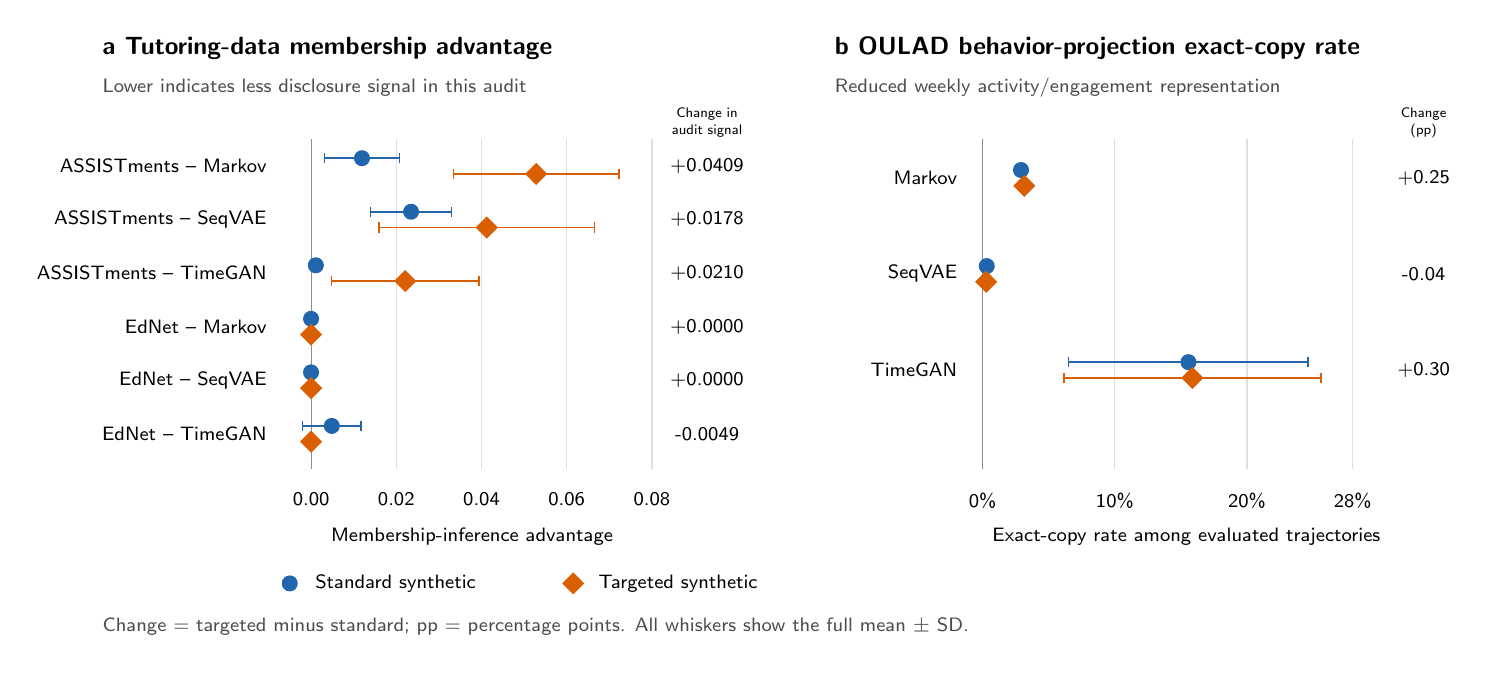
\begin{tikzpicture}[x=1cm,y=1cm,font=\sffamily]
\definecolor{auditblue}{HTML}{2166AC}
\definecolor{auditorange}{HTML}{D95F02}
\node[font=\sffamily\scriptsize,anchor=west,font=\sffamily\bfseries\small] at (0.20000,6.65000) {a  Tutoring-data membership advantage};
\node[font=\sffamily\scriptsize,anchor=west,font=\sffamily\bfseries\small] at (9.50000,6.65000) {b  OULAD behavior-projection exact-copy rate};
\node[font=\sffamily\scriptsize,anchor=west,text=black!70] at (0.20000,6.15000) {Lower indicates less disclosure signal in this audit};
\node[font=\sffamily\scriptsize,anchor=west,text=black!70] at (9.50000,6.15000) {Reduced weekly activity/engagement representation};
\node[font=\sffamily\scriptsize,align=center,font=\sffamily\tiny] at (8.00000,5.70000) {Change in\\audit signal};
\node[font=\sffamily\scriptsize,align=center,font=\sffamily\tiny] at (17.10000,5.70000) {Change\\(pp)};
\draw[black!45] (2.97059,1.30000) -- (2.97059,5.50000);
\node[font=\sffamily\scriptsize,anchor=north] at (2.97059,1.12000) {0.00};
\draw[gray!25] (4.05294,1.30000) -- (4.05294,5.50000);
\node[font=\sffamily\scriptsize,anchor=north] at (4.05294,1.12000) {0.02};
\draw[gray!25] (5.13529,1.30000) -- (5.13529,5.50000);
\node[font=\sffamily\scriptsize,anchor=north] at (5.13529,1.12000) {0.04};
\draw[gray!25] (6.21765,1.30000) -- (6.21765,5.50000);
\node[font=\sffamily\scriptsize,anchor=north] at (6.21765,1.12000) {0.06};
\draw[gray!25] (7.30000,1.30000) -- (7.30000,5.50000);
\node[font=\sffamily\scriptsize,anchor=north] at (7.30000,1.12000) {0.08};
\draw[black!45] (11.50000,1.30000) -- (11.50000,5.50000);
\node[font=\sffamily\scriptsize,anchor=north] at (11.50000,1.12000) {0\%};
\draw[gray!25] (13.17857,1.30000) -- (13.17857,5.50000);
\node[font=\sffamily\scriptsize,anchor=north] at (13.17857,1.12000) {10\%};
\draw[gray!25] (14.85714,1.30000) -- (14.85714,5.50000);
\node[font=\sffamily\scriptsize,anchor=north] at (14.85714,1.12000) {20\%};
\draw[gray!25] (16.20000,1.30000) -- (16.20000,5.50000);
\node[font=\sffamily\scriptsize,anchor=north] at (16.20000,1.12000) {28\%};
\node[font=\sffamily\scriptsize,anchor=east] at (2.53000,5.15000) {ASSISTments -- Markov};
\draw[auditblue,line width=.7pt] (3.14193,5.25000) -- (4.09217,5.25000);
\draw[auditblue,line width=.55pt] (3.14193,5.18500) -- (3.14193,5.31500);
\draw[auditblue,line width=.55pt] (4.09217,5.18500) -- (4.09217,5.31500);
\node[circle,draw=auditblue,fill=auditblue,inner sep=1.9pt] at (3.61705,5.25000) {};
\draw[auditorange,line width=.7pt] (4.77882,5.05000) -- (6.88028,5.05000);
\draw[auditorange,line width=.55pt] (4.77882,4.98500) -- (4.77882,5.11500);
\draw[auditorange,line width=.55pt] (6.88028,4.98500) -- (6.88028,5.11500);
\node[diamond,draw=auditorange,fill=auditorange,inner sep=1.9pt] at (5.82955,5.05000) {};
\node[font=\sffamily\scriptsize,] at (8.00000,5.15000) {+0.0409};
\node[font=\sffamily\scriptsize,anchor=east] at (2.53000,4.47000) {ASSISTments -- SeqVAE};
\draw[auditblue,line width=.7pt] (3.72577,4.57000) -- (4.75583,4.57000);
\draw[auditblue,line width=.55pt] (3.72577,4.50500) -- (3.72577,4.63500);
\draw[auditblue,line width=.55pt] (4.75583,4.50500) -- (4.75583,4.63500);
\node[circle,draw=auditblue,fill=auditblue,inner sep=1.9pt] at (4.24080,4.57000) {};
\draw[auditorange,line width=.7pt] (3.83356,4.37000) -- (6.56953,4.37000);
\draw[auditorange,line width=.55pt] (3.83356,4.30500) -- (3.83356,4.43500);
\draw[auditorange,line width=.55pt] (6.56953,4.30500) -- (6.56953,4.43500);
\node[diamond,draw=auditorange,fill=auditorange,inner sep=1.9pt] at (5.20154,4.37000) {};
\node[font=\sffamily\scriptsize,] at (8.00000,4.47000) {+0.0178};
\node[font=\sffamily\scriptsize,anchor=east] at (2.53000,3.79000) {ASSISTments -- TimeGAN};
\draw[auditblue,line width=.7pt] (2.98159,3.89000) -- (3.08028,3.89000);
\draw[auditblue,line width=.55pt] (2.98159,3.82500) -- (2.98159,3.95500);
\draw[auditblue,line width=.55pt] (3.08028,3.82500) -- (3.08028,3.95500);
\node[circle,draw=auditblue,fill=auditblue,inner sep=1.9pt] at (3.03093,3.89000) {};
\draw[auditorange,line width=.7pt] (3.22907,3.69000) -- (5.10349,3.69000);
\draw[auditorange,line width=.55pt] (3.22907,3.62500) -- (3.22907,3.75500);
\draw[auditorange,line width=.55pt] (5.10349,3.62500) -- (5.10349,3.75500);
\node[diamond,draw=auditorange,fill=auditorange,inner sep=1.9pt] at (4.16628,3.69000) {};
\node[font=\sffamily\scriptsize,] at (8.00000,3.79000) {+0.0210};
\node[font=\sffamily\scriptsize,anchor=east] at (2.53000,3.11000) {EdNet -- Markov};
\draw[auditblue,line width=.7pt] (2.97059,3.21000) -- (2.97059,3.21000);
\draw[auditblue,line width=.55pt] (2.97059,3.14500) -- (2.97059,3.27500);
\draw[auditblue,line width=.55pt] (2.97059,3.14500) -- (2.97059,3.27500);
\node[circle,draw=auditblue,fill=auditblue,inner sep=1.9pt] at (2.97059,3.21000) {};
\draw[auditorange,line width=.7pt] (2.97059,3.01000) -- (2.97059,3.01000);
\draw[auditorange,line width=.55pt] (2.97059,2.94500) -- (2.97059,3.07500);
\draw[auditorange,line width=.55pt] (2.97059,2.94500) -- (2.97059,3.07500);
\node[diamond,draw=auditorange,fill=auditorange,inner sep=1.9pt] at (2.97059,3.01000) {};
\node[font=\sffamily\scriptsize,] at (8.00000,3.11000) {+0.0000};
\node[font=\sffamily\scriptsize,anchor=east] at (2.53000,2.43000) {EdNet -- SeqVAE};
\draw[auditblue,line width=.7pt] (2.97059,2.53000) -- (2.97059,2.53000);
\draw[auditblue,line width=.55pt] (2.97059,2.46500) -- (2.97059,2.59500);
\draw[auditblue,line width=.55pt] (2.97059,2.46500) -- (2.97059,2.59500);
\node[circle,draw=auditblue,fill=auditblue,inner sep=1.9pt] at (2.97059,2.53000) {};
\draw[auditorange,line width=.7pt] (2.97059,2.33000) -- (2.97059,2.33000);
\draw[auditorange,line width=.55pt] (2.97059,2.26500) -- (2.97059,2.39500);
\draw[auditorange,line width=.55pt] (2.97059,2.26500) -- (2.97059,2.39500);
\node[diamond,draw=auditorange,fill=auditorange,inner sep=1.9pt] at (2.97059,2.33000) {};
\node[font=\sffamily\scriptsize,] at (8.00000,2.43000) {+0.0000};
\node[font=\sffamily\scriptsize,anchor=east] at (2.53000,1.75000) {EdNet -- TimeGAN};
\draw[auditblue,line width=.7pt] (2.86152,1.85000) -- (3.60628,1.85000);
\draw[auditblue,line width=.55pt] (2.86152,1.78500) -- (2.86152,1.91500);
\draw[auditblue,line width=.55pt] (3.60628,1.78500) -- (3.60628,1.91500);
\node[circle,draw=auditblue,fill=auditblue,inner sep=1.9pt] at (3.23390,1.85000) {};
\draw[auditorange,line width=.7pt] (2.97059,1.65000) -- (2.97059,1.65000);
\draw[auditorange,line width=.55pt] (2.97059,1.58500) -- (2.97059,1.71500);
\draw[auditorange,line width=.55pt] (2.97059,1.58500) -- (2.97059,1.71500);
\node[diamond,draw=auditorange,fill=auditorange,inner sep=1.9pt] at (2.97059,1.65000) {};
\node[font=\sffamily\scriptsize,] at (8.00000,1.75000) {-0.0049};
\node[font=\sffamily\scriptsize,anchor=east] at (11.30000,5.00000) {Markov};
\draw[auditblue,line width=.7pt] (11.97108,5.10000) -- (12.00249,5.10000);
\draw[auditblue,line width=.55pt] (11.97108,5.03500) -- (11.97108,5.16500);
\draw[auditblue,line width=.55pt] (12.00249,5.03500) -- (12.00249,5.16500);
\node[circle,draw=auditblue,fill=auditblue,inner sep=1.9pt] at (11.98679,5.10000) {};
\draw[auditorange,line width=.7pt] (12.01968,4.90000) -- (12.03782,4.90000);
\draw[auditorange,line width=.55pt] (12.01968,4.83500) -- (12.01968,4.96500);
\draw[auditorange,line width=.55pt] (12.03782,4.83500) -- (12.03782,4.96500);
\node[diamond,draw=auditorange,fill=auditorange,inner sep=1.9pt] at (12.02875,4.90000) {};
\node[font=\sffamily\scriptsize,] at (17.10000,5.00000) {+0.25};
\node[font=\sffamily\scriptsize,anchor=east] at (11.30000,3.78000) {SeqVAE};
\draw[auditblue,line width=.7pt] (11.53631,3.88000) -- (11.56721,3.88000);
\draw[auditblue,line width=.55pt] (11.53631,3.81500) -- (11.53631,3.94500);
\draw[auditblue,line width=.55pt] (11.56721,3.81500) -- (11.56721,3.94500);
\node[circle,draw=auditblue,fill=auditblue,inner sep=1.9pt] at (11.55176,3.88000) {};
\draw[auditorange,line width=.7pt] (11.53953,3.68000) -- (11.55000,3.68000);
\draw[auditorange,line width=.55pt] (11.53953,3.61500) -- (11.53953,3.74500);
\draw[auditorange,line width=.55pt] (11.55000,3.61500) -- (11.55000,3.74500);
\node[diamond,draw=auditorange,fill=auditorange,inner sep=1.9pt] at (11.54476,3.68000) {};
\node[font=\sffamily\scriptsize,] at (17.10000,3.78000) {-0.04};
\node[font=\sffamily\scriptsize,anchor=east] at (11.30000,2.56000) {TimeGAN};
\draw[auditblue,line width=.7pt] (12.59201,2.66000) -- (15.63394,2.66000);
\draw[auditblue,line width=.55pt] (12.59201,2.59500) -- (12.59201,2.72500);
\draw[auditblue,line width=.55pt] (15.63394,2.59500) -- (15.63394,2.72500);
\node[circle,draw=auditblue,fill=auditblue,inner sep=1.9pt] at (14.11298,2.66000) {};
\draw[auditorange,line width=.7pt] (12.53029,2.46000) -- (15.79637,2.46000);
\draw[auditorange,line width=.55pt] (12.53029,2.39500) -- (12.53029,2.52500);
\draw[auditorange,line width=.55pt] (15.79637,2.39500) -- (15.79637,2.52500);
\node[diamond,draw=auditorange,fill=auditorange,inner sep=1.9pt] at (14.16333,2.46000) {};
\node[font=\sffamily\scriptsize,] at (17.10000,2.56000) {+0.30};
\node[font=\sffamily\scriptsize,anchor=west] at (3.10000,0.45000) {Membership-inference advantage};
\node[font=\sffamily\scriptsize,anchor=west] at (11.50000,0.45000) {Exact-copy rate among evaluated trajectories};
\node[circle,draw=auditblue,fill=auditblue,inner sep=1.9pt] at (2.7,-.15) {};
\node[diamond,draw=auditorange,fill=auditorange,inner sep=1.9pt] at (6.3,-.15) {};
\node[font=\sffamily\scriptsize,anchor=west] at (2.90000,-0.15000) {Standard synthetic};
\node[font=\sffamily\scriptsize,anchor=west] at (6.50000,-0.15000) {Targeted synthetic};
\node[font=\sffamily\scriptsize,anchor=west,text=black!70] at (0.20000,-0.70000) {Change = targeted minus standard; pp = percentage points. All whiskers show the full mean $\pm$ SD.};
\end{tikzpicture}
}
\caption{Supporting dataset-level disclosure-risk audit. Panel (a) reports membership-inference advantage for full normalized tutoring trajectories over the declared audit columns. Panel (b) reports exact copying for the OULAD dominant-activity/engagement projection; full-record membership inference is not generator-comparable there. The change in audit signal is targeted minus standard; positive values indicate a larger tested indicator after targeting. Points are means and whiskers show the full mean $\pm$ population SD across three seeds; a descriptive SD whisker may extend below zero. The audit does not estimate disclosure risk specifically for learners on uncommon pathways. These are empirical memorization indicators, not formal privacy guarantees.}
\label{fig:rq2-disclosure-risk}
\end{figure}

\ifdefined\embeddedappendix
\else
\bibliographystyle{apacite-apa7}
\bibliography{references}
\end{document}
\fi
